% ผลจากรายงานที่ผู้ใช้ส่ง ไม่ได้รันทดสอบแอปใหม่ระหว่างจัดทำเอกสาร
\section{ผลการตรวจสอบ System Functional Test ฝั่ง Frontend}
\label{sec:frontend-test-results}

การตรวจสอบฝั่ง Frontend นำเสนอผลตามวิธีการทดสอบในหัวข้อ~\ref{sec:frontend-test-method} โดยใช้รายงานรวมและรายงานรายละเอียดของโครงงานเป็นหลักฐาน แบ่งการนำเสนอเป็นผลรวมของชุดทดสอบและผลการตรวจเส้นทางใช้งานแต่ละชุด พร้อมภาพหน้าจอจากรอบทดสอบจริง

\subsection{ผลการทดสอบด้วย System Functional Test}

รายงานรวมจัดกลุ่มผลการตรวจเป็น 12 ชุด ใช้รหัส FT-01 ถึง FT-03 และ FT-06 ถึง FT-14 ตามต้นฉบับ ดังตารางที่~\ref{tab:flutter-test-overview} ผลที่รายงานเป็นผลตามขอบเขตที่ตรวจจริงของแต่ละชุด โดยรายงานรายละเอียดระบุการ Flutter Integration Test กับแอปพลิเคชันและ API จริง และรายงานผลตามขอบเขตที่ตรวจสอบในแต่ละชุด

\begingroup
\small
\renewcommand{\arraystretch}{1.15}
\begin{longtable}{|>{\raggedright\arraybackslash}p{0.08\textwidth}|>{\raggedright\arraybackslash}p{0.16\textwidth}|>{\raggedright\arraybackslash}p{0.36\textwidth}|>{\raggedright\arraybackslash}p{0.12\textwidth}|>{\raggedright\arraybackslash}p{0.12\textwidth}|}
\caption{สรุปผลการตรวจสอบ System Functional ฝั่ง Frontend}\label{tab:flutter-test-overview}\\ \hline
\textbf{รหัส} & \textbf{ชุดทดสอบ} & \textbf{ผลที่ตรวจจริง} & \textbf{ผล} & \textbf{รายละเอียด} \\ \hline
\endfirsthead
\multicolumn{5}{c}{สรุปผลการตรวจสอบ System Functional ฝั่ง Frontend (ต่อ)} \\ \hline
\textbf{รหัส} & \textbf{ชุดทดสอบ} & \textbf{ผลที่ตรวจจริง} & \textbf{ผล} & \textbf{รายละเอียด} \\ \hline
\endhead
\endfoot
\endlastfoot
FT-01 & สมัครสมาชิก Onboarding และ Daily Wellness & ยอมรับนโยบาย ยืนยัน OTP ทำ Onboarding ครบ กรอก Wellness และเปิดโปรไฟล์สำเร็จ & ผ่าน & ตารางที่~\ref{tab:flutter-ft-01} \\ \hline
FT-02 & โปรแกรมและตารางฝึกซ้อม & ใช้โปรแกรมที่สมัครค้างไว้ วาง Easy 3 วันและ Long 1 วัน บันทึกและเปิดหน้าตรวจใหม่ตรงกัน ตารางไม่ครบหรือ Easy เกินโควตาไม่ผ่าน & ผ่าน & ตารางที่~\ref{tab:flutter-ft-02} \\ \hline
FT-03 & วิ่งในลู่และ Park สรุปผล รางวัล สถิติ และประวัติ & เลือกลู่ \ensuremath{\rightarrow} ระหว่างวิ่ง/พัก \ensuremath{\rightarrow} จบลู่ \ensuremath{\rightarrow} เลือก Park \ensuremath{\rightarrow} ระหว่างวิ่งพร้อม GPS \ensuremath{\rightarrow} จบ Park \ensuremath{\rightarrow} รับรางวัล 5 เหรียญตรงยอดจริง \ensuremath{\rightarrow} ดูสถิติ \ensuremath{\rightarrow} เปิดรายละเอียดประวัติหลังโหลดข้อมูลจริง & ผ่าน & ตารางที่~\ref{tab:flutter-ft-03} \\ \hline
FT-06 & ข้อมูลโปรไฟล์ ชื่อ และ UID & ตรวจชื่อช่องว่าง บันทึกชื่อ แสดงชื่อบนหน้าหลัก และคืนชื่อเดิมได้ & ผ่าน & ตารางที่~\ref{tab:flutter-ft-06} \\ \hline
FT-07 & เปลี่ยนภาพโปรไฟล์ & เลือกภาพล่าสุดในเครื่อง อัปโหลดและถอดรหัสภาพบนหน้าจอได้ เปิดโปรไฟล์ใหม่ยังเป็นภาพเดียวกัน ชื่อและ UID ไม่เปลี่ยน & ผ่าน & ตารางที่~\ref{tab:flutter-ft-07} \\ \hline
FT-08 & เพื่อน: ส่งคำขอ & UID ผิด/ตนเองถูกปฏิเสธ ส่ง UID ตัวเล็กได้ ส่งซ้ำถูกปฏิเสธ และยกเลิกคำขอได้ & ผ่าน & ตารางที่~\ref{tab:flutter-ft-08} \\ \hline
FT-09 & เพื่อน: บัญชีรองตอบรับ & เห็นคำขอจากบัญชีหลักถูก ID ตอบรับแล้วเห็นบัญชีหลักเป็นเพื่อนหนึ่งรายการ & ผ่าน & ตารางที่~\ref{tab:flutter-ft-09} \\ \hline
FT-10 & เพื่อน: ตรวจกลับบัญชีหลัก & เห็นบัญชีรองเป็นเพื่อนหนึ่งรายการ ความสัมพันธ์ ID เดียวกัน และไม่มีคำขอส่งค้าง & ผ่าน & ตารางที่~\ref{tab:flutter-ft-10} \\ \hline
FT-11 & คลับ: สร้างคลับ & ชื่อว่างถูกปฏิเสธ สร้างคลับชื่อ/คำอธิบายตรงข้อมูล บัญชีหลักเป็นหัวหน้า สมาชิกเริ่มต้น 1 คน & ผ่าน & ตารางที่~\ref{tab:flutter-ft-11} \\ \hline
FT-12 & คลับ: ค้นหาและขอเข้าร่วม & บัญชีรองค้นคลับถูก ID ส่งคำขอรออนุมัติ ปุ่มส่งซ้ำถูกปิด ก่อนอนุมัติยังไม่มีสมาชิกเพิ่ม & ผ่าน & ตารางที่~\ref{tab:flutter-ft-12} \\ \hline
FT-13 & คลับ: อนุมัติคำขอ & บัญชีหลักอนุมัติแล้วสมาชิกเพิ่มจาก 1 เป็น 2 รองเป็นสมาชิกหนึ่งรายการ หัวหน้าหนึ่งคน และคำขอหาย & ผ่าน & ตารางที่~\ref{tab:flutter-ft-13} \\ \hline
FT-14 & ร้านค้าและ Avatar & เหรียญไม่พอซื้อไม่ได้ ลองใส่ไม่ทับชุดเดิม ซื้อเสื้อม่วง 15 เหรียญจากยอด 15 เหลือ 0 มีใบซื้อหนึ่งรายการ สวมใส่และบันทึกแล้ว Home/หน้าแต่งตัวใหม่ยังใช้ชุดนั้น & ผ่าน & ตารางที่~\ref{tab:flutter-ft-14} \\ \hline
\end{longtable}
\endgroup

\subsection{ผลการทดสอบเส้นทางใช้งานด้วย Flutter Integration Test}

รายงานแต่ละชุดบันทึกจุดตรวจระหว่างการใช้งานแอปพลิเคชันและการเชื่อมต่อ API จริง รวมถึงการกรอก OTP แล้วให้ชุดทดสอบตรวจสถานะหรือข้อมูลจาก API และบันทึกภาพโดยอัตโนมัติ
\subsubsection{FT-01 สมัครสมาชิก Onboarding และ Daily Wellness}

ผลครอบคลุมการสมัครสมาชิก การยืนยัน OTP การกรอกข้อมูลเริ่มต้นครบ 4 ขั้นตอน การเข้าสู่หน้าหลัก การบันทึกสุขภาวะ และการเปิดโปรไฟล์

\begingroup
\small
\renewcommand{\arraystretch}{1.15}
\begin{longtable}{|>{\raggedright\arraybackslash}p{0.07\textwidth}|>{\raggedright\arraybackslash}p{0.57\textwidth}|>{\raggedright\arraybackslash}p{0.08\textwidth}|>{\raggedright\arraybackslash}p{0.16\textwidth}|}
\caption{ผลการทดสอบ FT-01}\label{tab:flutter-ft-01}\\ \hline
\textbf{ลำดับ} & \textbf{จุดตรวจและผลที่ได้รับจริง} & \textbf{ผล} & \textbf{หลักฐาน} \\ \hline
\endfirsthead
\multicolumn{4}{c}{ผลการทดสอบ FT-01 (ต่อ)} \\ \hline
\textbf{ลำดับ} & \textbf{จุดตรวจและผลที่ได้รับจริง} & \textbf{ผล} & \textbf{หลักฐาน} \\ \hline
\endhead
\endfoot
\endlastfoot
1 & เปิดหน้าเข้าสู่ระบบได้เมื่อไม่มีเซสชันที่บันทึกไว้ & ผ่าน & ภาพที่~\ref{fig:flutter-ft-01-1} (a) \\ \hline
2 & หน้าสมัครสมาชิกรับชื่อและอีเมลของบัญชีทดสอบได้ & ผ่าน & ภาพที่~\ref{fig:flutter-ft-01-1} (b) \\ \hline
3 & ยังดำเนินการต่อไม่ได้ก่อนยอมรับนโยบาย & ผ่าน & ภาพที่~\ref{fig:flutter-ft-01-1} (c) \\ \hline
4 & การยอมรับนโยบายทำให้ปุ่มดำเนินการต่อใช้งานได้ & ผ่าน & ภาพที่~\ref{fig:flutter-ft-01-2} (a) \\ \hline
5 & ส่งคำขอรหัส OTP สำหรับสมัครสมาชิกไปยังอีเมลที่กำหนดได้ & ผ่าน & ภาพที่~\ref{fig:flutter-ft-01-2} (b) \\ \hline
6 & ยืนยัน OTP สำเร็จและเข้าสู่ขั้นตอนกรอกข้อมูลเริ่มต้น & ผ่าน & ภาพที่~\ref{fig:flutter-ft-01-2} (c) \\ \hline
7 & ข้อมูลจำลอง ได้แก่ วันเกิด เพศ น้ำหนัก ส่วนสูง และจำนวนวันฝึก ผ่านการตรวจข้อมูล & ผ่าน & ภาพที่~\ref{fig:flutter-ft-01-3} (a) \\ \hline
8 & เลือกคำตอบจำลองว่าไม่มีโรคประจำตัวและไม่มีประวัติบาดเจ็บได้ & ผ่าน & ภาพที่~\ref{fig:flutter-ft-01-3} (b) \\ \hline
9 & เลือกเฉพาะเป้าหมายเพิ่มความอึด โดยไม่กำหนดเป้าหมายระยะทาง & ผ่าน & ภาพที่~\ref{fig:flutter-ft-01-3} (c) \\ \hline
10 & เลือกประวัติการวิ่งจำลองสำหรับผู้เริ่มต้นได้ & ผ่าน & ภาพที่~\ref{fig:flutter-ft-01-4} (a) \\ \hline
11 & กรอกข้อมูลเริ่มต้นครบและหน้าหลักแสดงบัญชีทดสอบ & ผ่าน & ภาพที่~\ref{fig:flutter-ft-01-4} (b) \\ \hline
12 & กรอกคะแนนสุขภาวะที่บังคับครบ 5 รายการแล้วปุ่มบันทึกใช้งานได้ & ผ่าน & ภาพที่~\ref{fig:flutter-ft-01-4} (c) \\ \hline
13 & API จริงรับข้อมูลสุขภาวะและหน้าหลักปรับสถานะตามข้อมูลที่บันทึก & ผ่าน & ภาพที่~\ref{fig:flutter-ft-01-5} (a) \\ \hline
14 & หน้าโปรไฟล์แสดงบัญชีทดสอบและ UID สาธารณะ โดยไม่มีข้อผิดพลาดที่ต้องลองใหม่ & ผ่าน & ภาพที่~\ref{fig:flutter-ft-01-5} (b) \\ \hline
\end{longtable}
\endgroup

\begin{figure}[H]
\centering
\begin{subfigure}[t]{0.31\textwidth}\centering

\includegraphics[width=\linewidth,height=0.43\textheight,keepaspectratio]{images/frontend_tests/ft-01-01-01-login.png}
\caption{เข้าสู่ระบบ}\end{subfigure}
\hfill
\begin{subfigure}[t]{0.31\textwidth}\centering

\includegraphics[width=\linewidth,height=0.43\textheight,keepaspectratio]{images/frontend_tests/ft-01-02-02-register.png}
\caption{สมัครสมาชิก}\end{subfigure}
\hfill
\begin{subfigure}[t]{0.31\textwidth}\centering

\includegraphics[width=\linewidth,height=0.43\textheight,keepaspectratio]{images/frontend_tests/ft-01-03-03-terms-disabled.png}
\caption{ยังไม่ยอมรับนโยบาย}\end{subfigure}
\caption{ภาพหลักฐาน FT-01 ชุดที่ 1}\label{fig:flutter-ft-01-1}
\end{figure}

\begin{figure}[H]
\centering
\begin{subfigure}[t]{0.31\textwidth}\centering

\includegraphics[width=\linewidth,height=0.43\textheight,keepaspectratio]{images/frontend_tests/ft-01-04-04-terms-consented.png}
\caption{ยอมรับนโยบาย}\end{subfigure}
\hfill
\begin{subfigure}[t]{0.31\textwidth}\centering

\includegraphics[width=\linewidth,height=0.43\textheight,keepaspectratio]{images/frontend_tests/ft-01-05-05-otp-requested.png}
\caption{ขอรหัส OTP}\end{subfigure}
\hfill
\begin{subfigure}[t]{0.31\textwidth}\centering
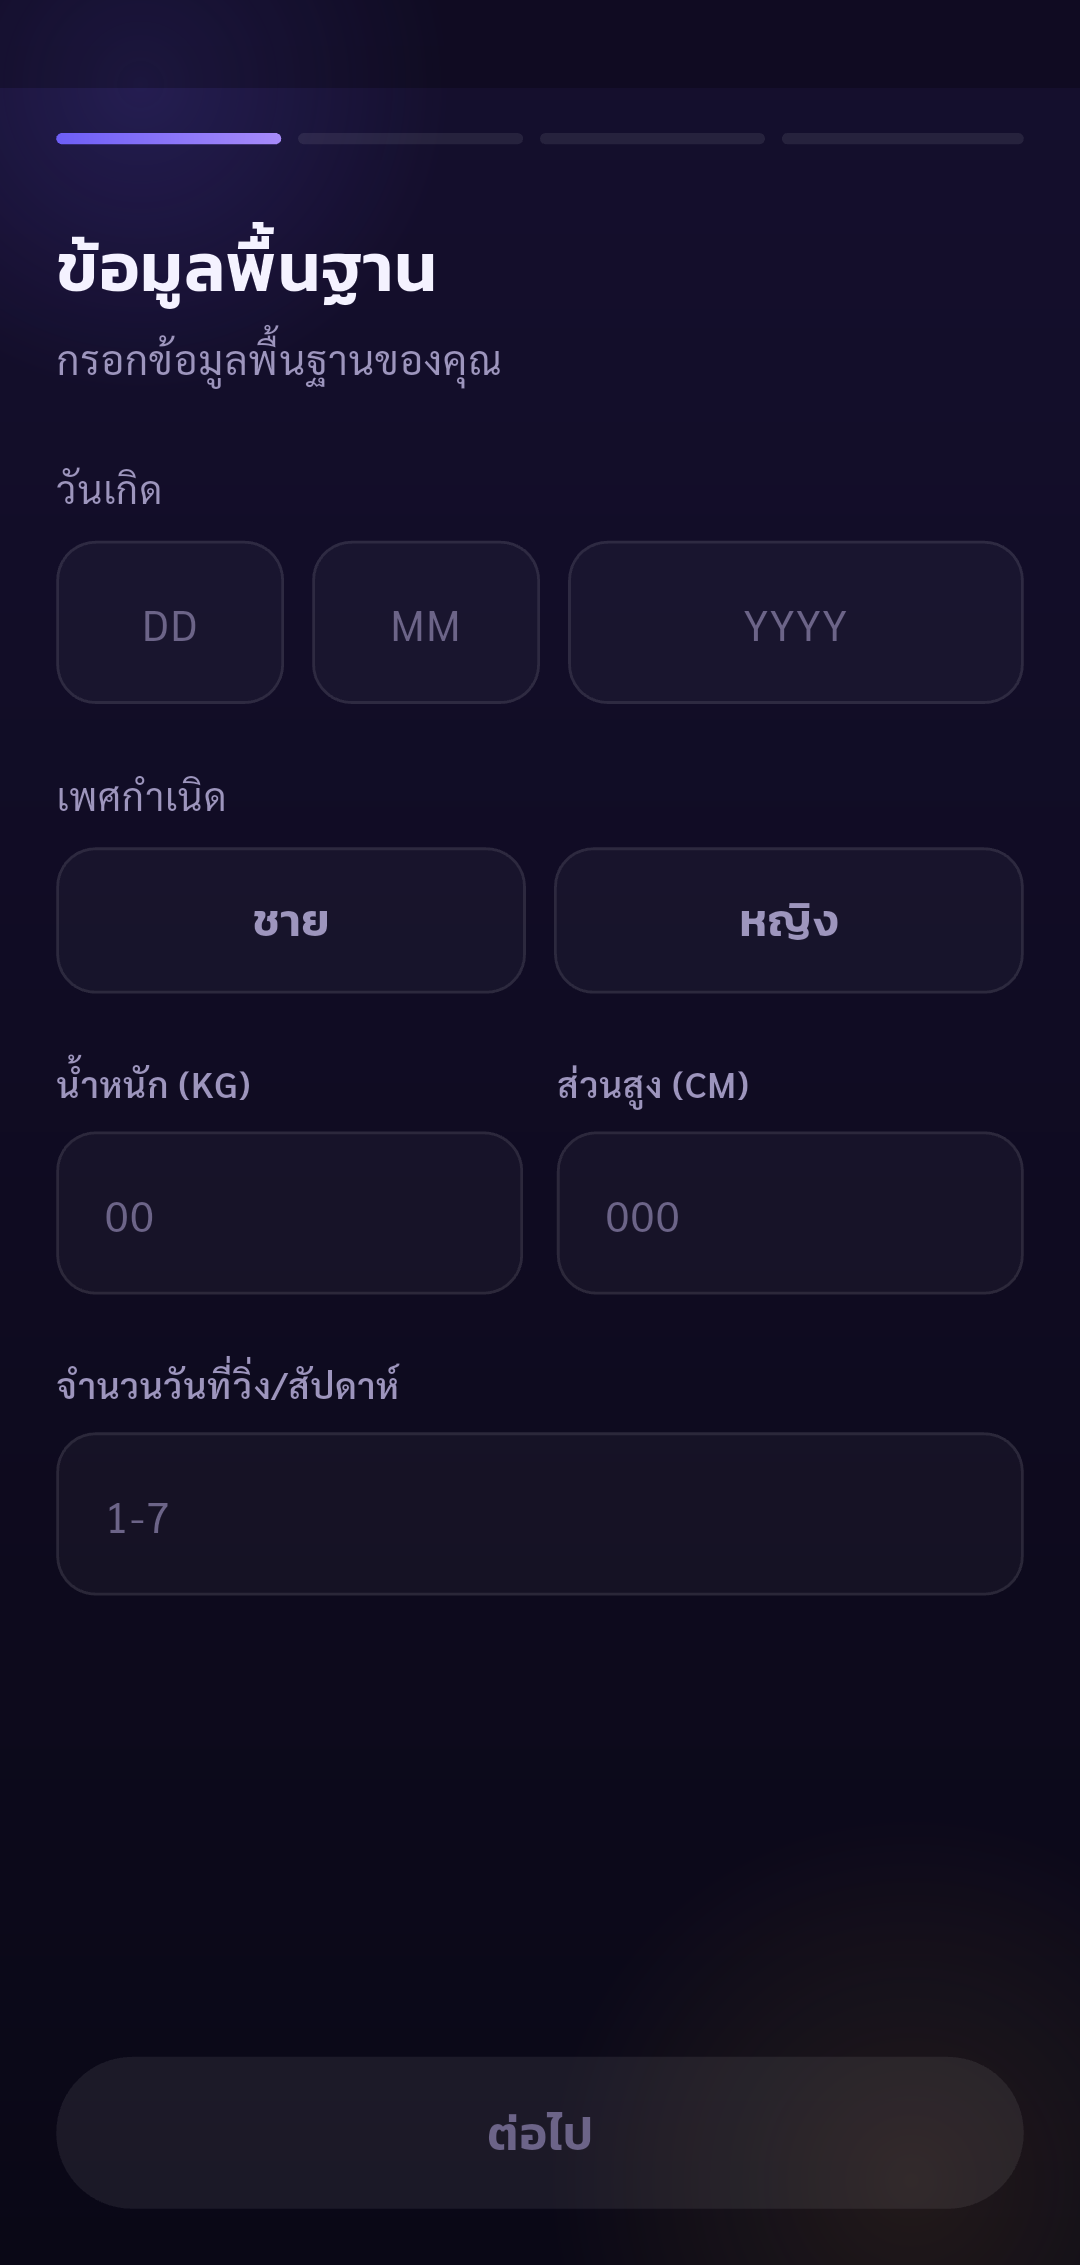
\includegraphics[width=\linewidth,height=0.43\textheight,keepaspectratio]{images/frontend_tests/ft-01-06-06-otp-verified.png}
\caption{ยืนยัน OTP}\end{subfigure}
\caption{ภาพหลักฐาน FT-01 ชุดที่ 2}\label{fig:flutter-ft-01-2}
\end{figure}

\begin{figure}[H]
\centering
\begin{subfigure}[t]{0.31\textwidth}\centering
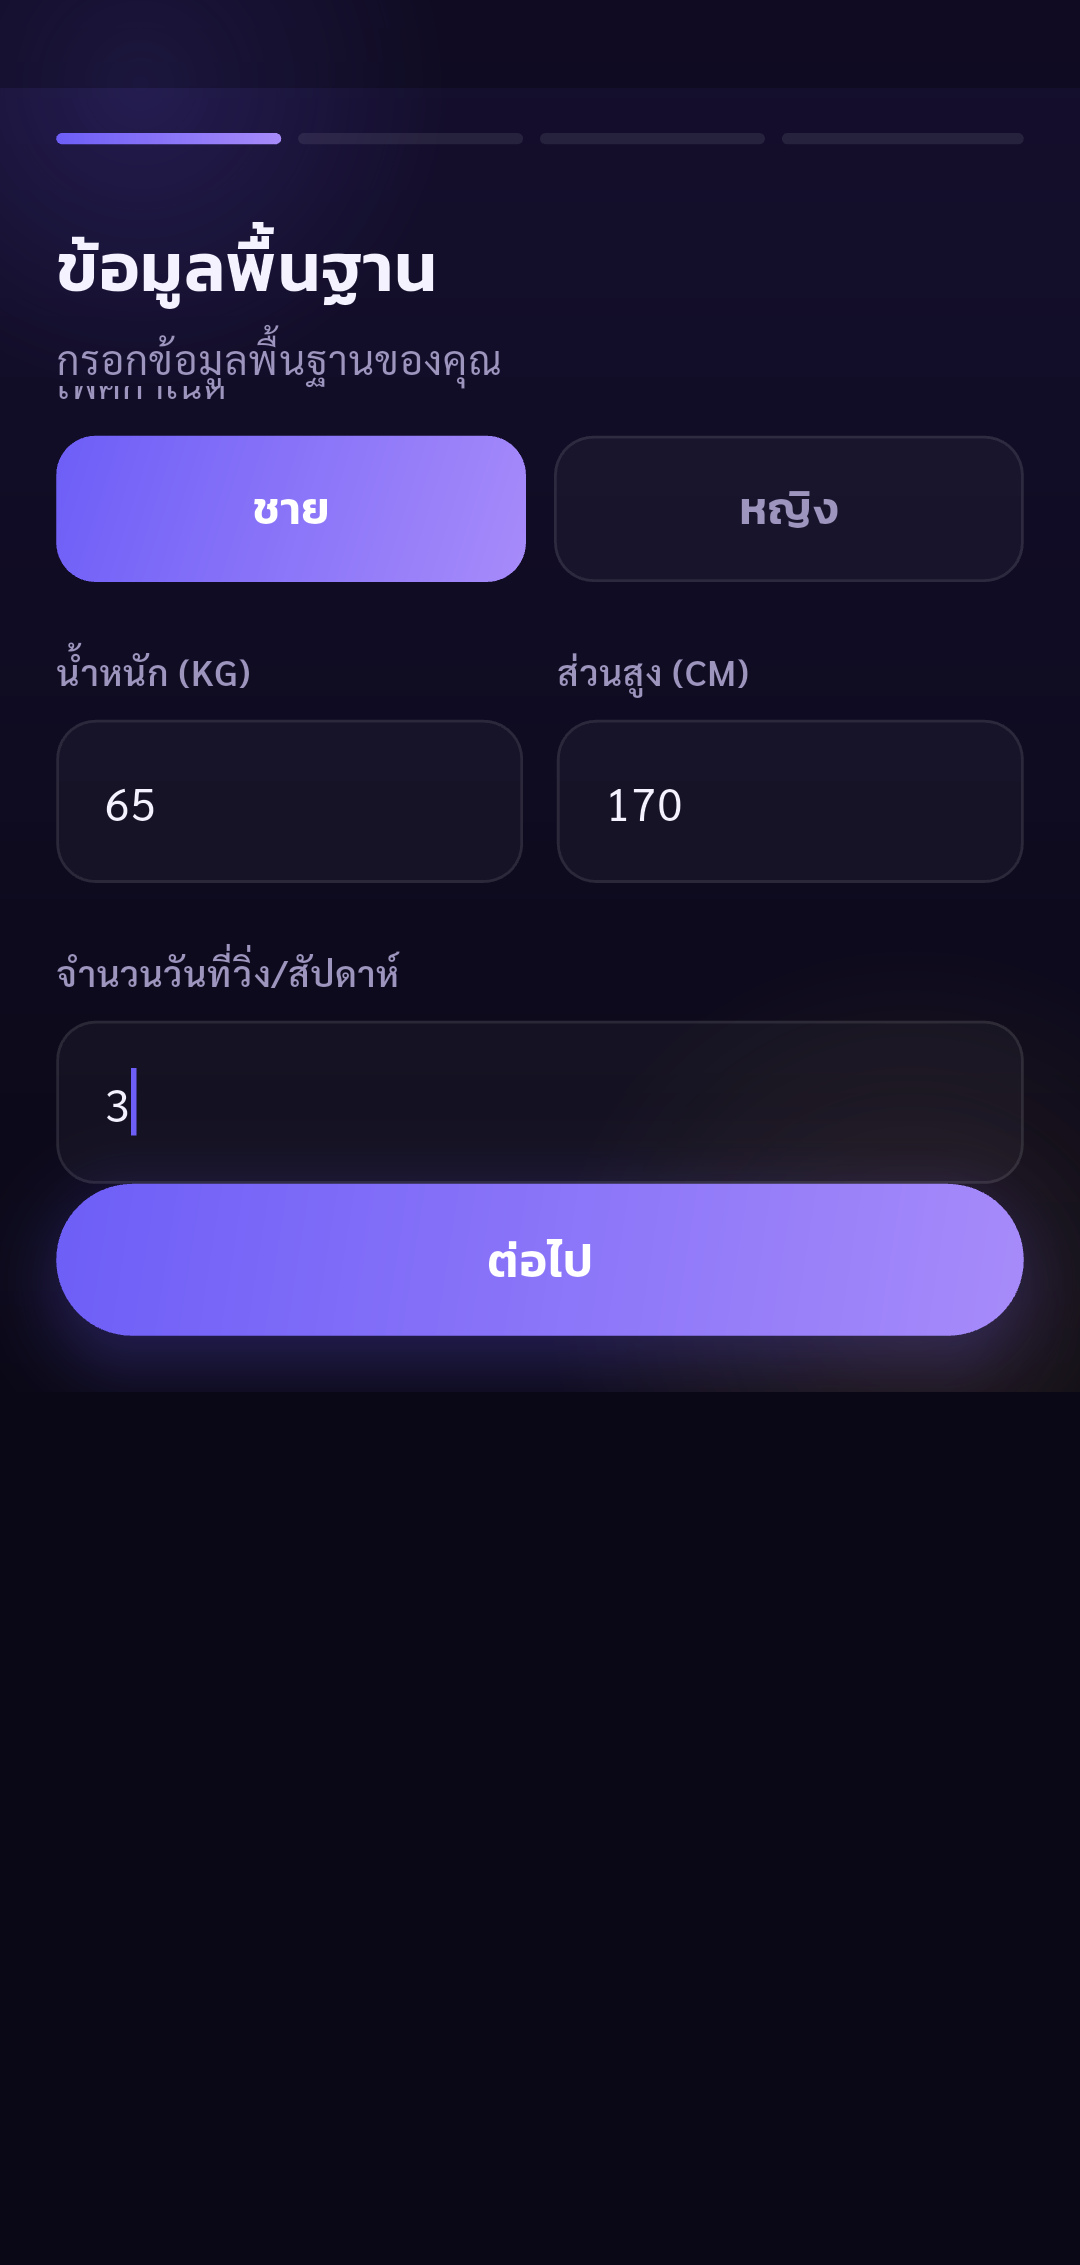
\includegraphics[width=\linewidth,height=0.43\textheight,keepaspectratio]{images/frontend_tests/ft-01-07-07-basic-valid.png}
\caption{ข้อมูลพื้นฐาน}\end{subfigure}
\hfill
\begin{subfigure}[t]{0.31\textwidth}\centering
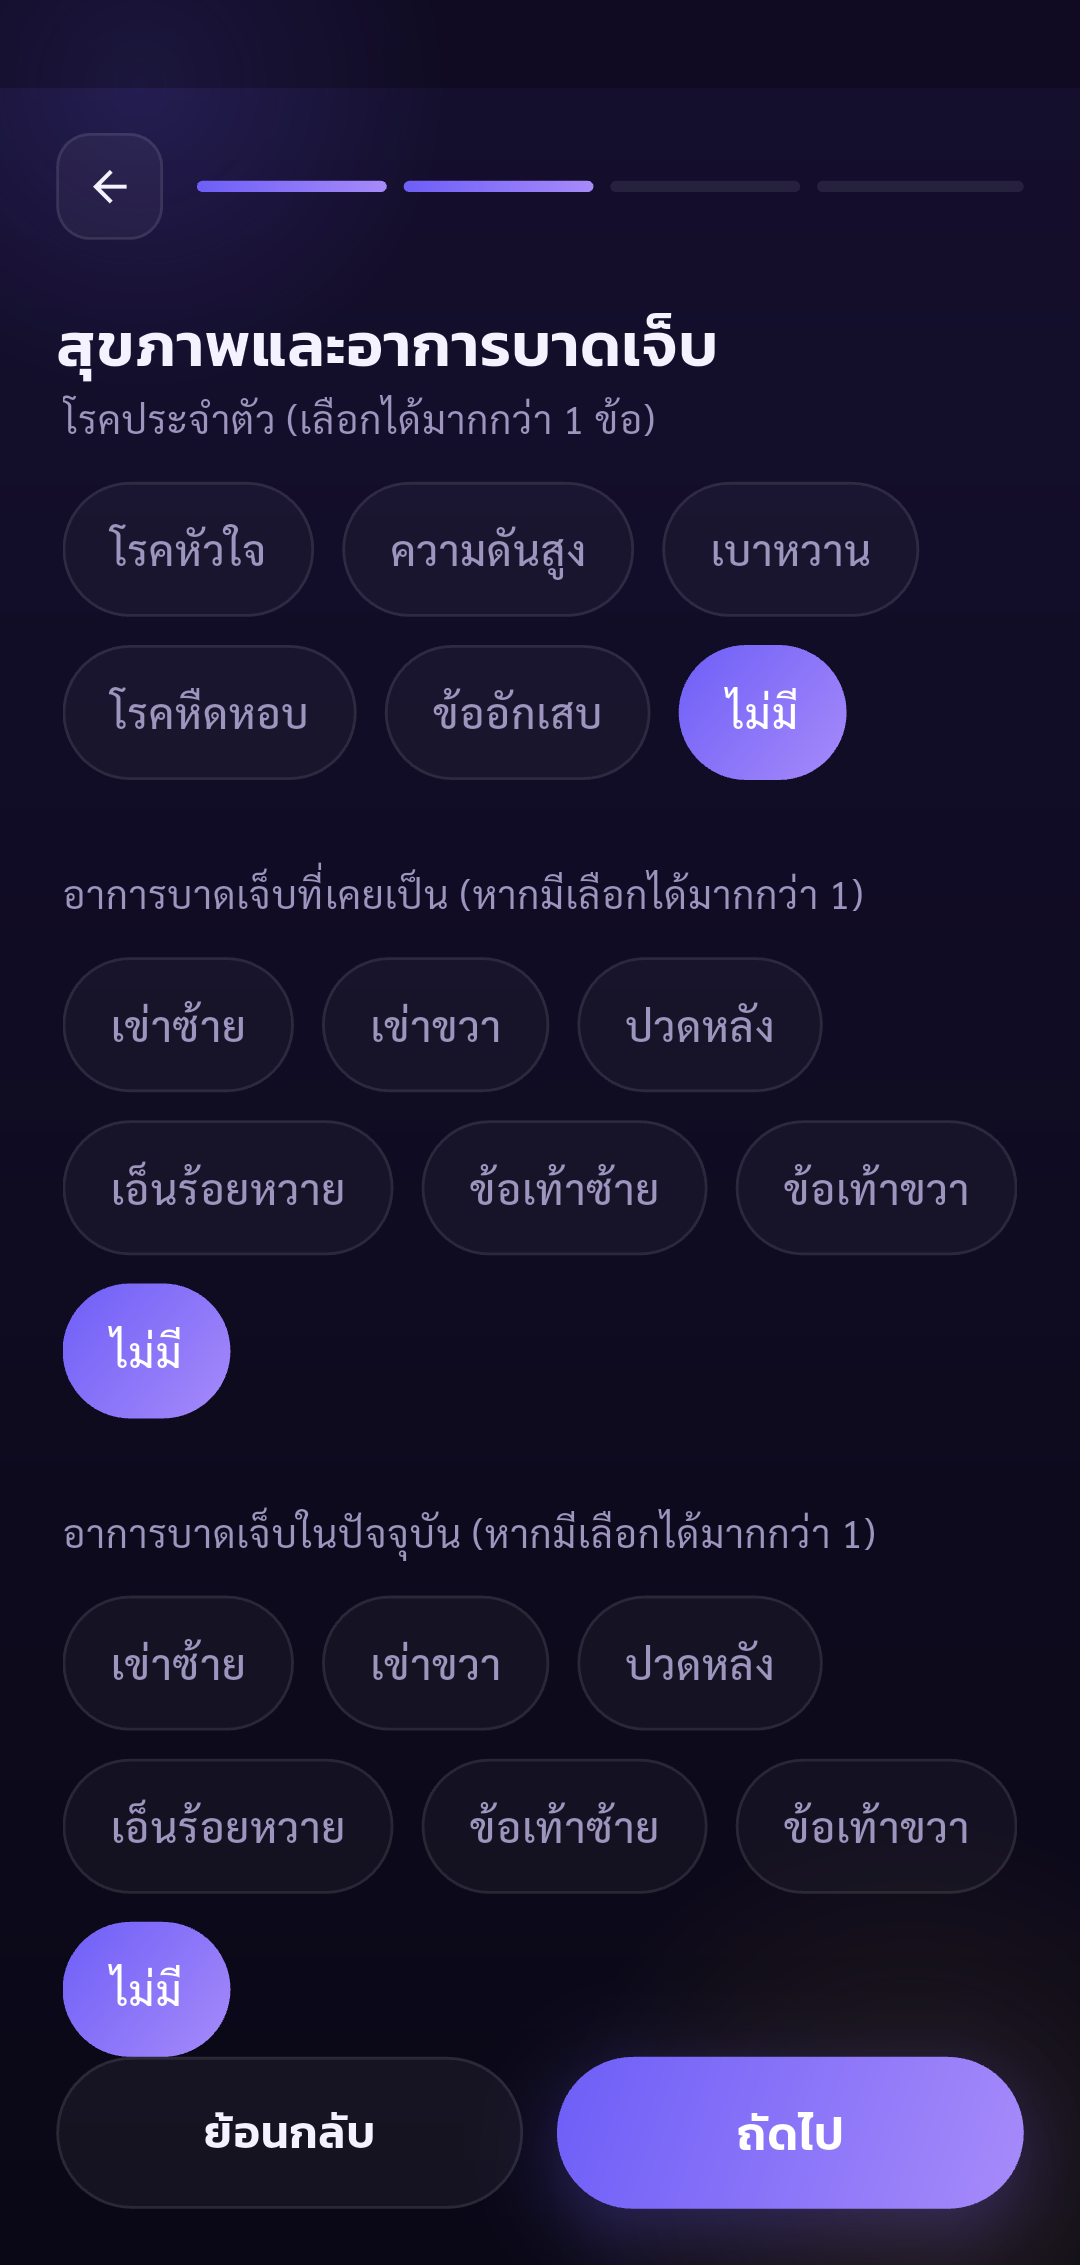
\includegraphics[width=\linewidth,height=0.43\textheight,keepaspectratio]{images/frontend_tests/ft-01-08-08-health.png}
\caption{ข้อมูลสุขภาพ}\end{subfigure}
\hfill
\begin{subfigure}[t]{0.31\textwidth}\centering
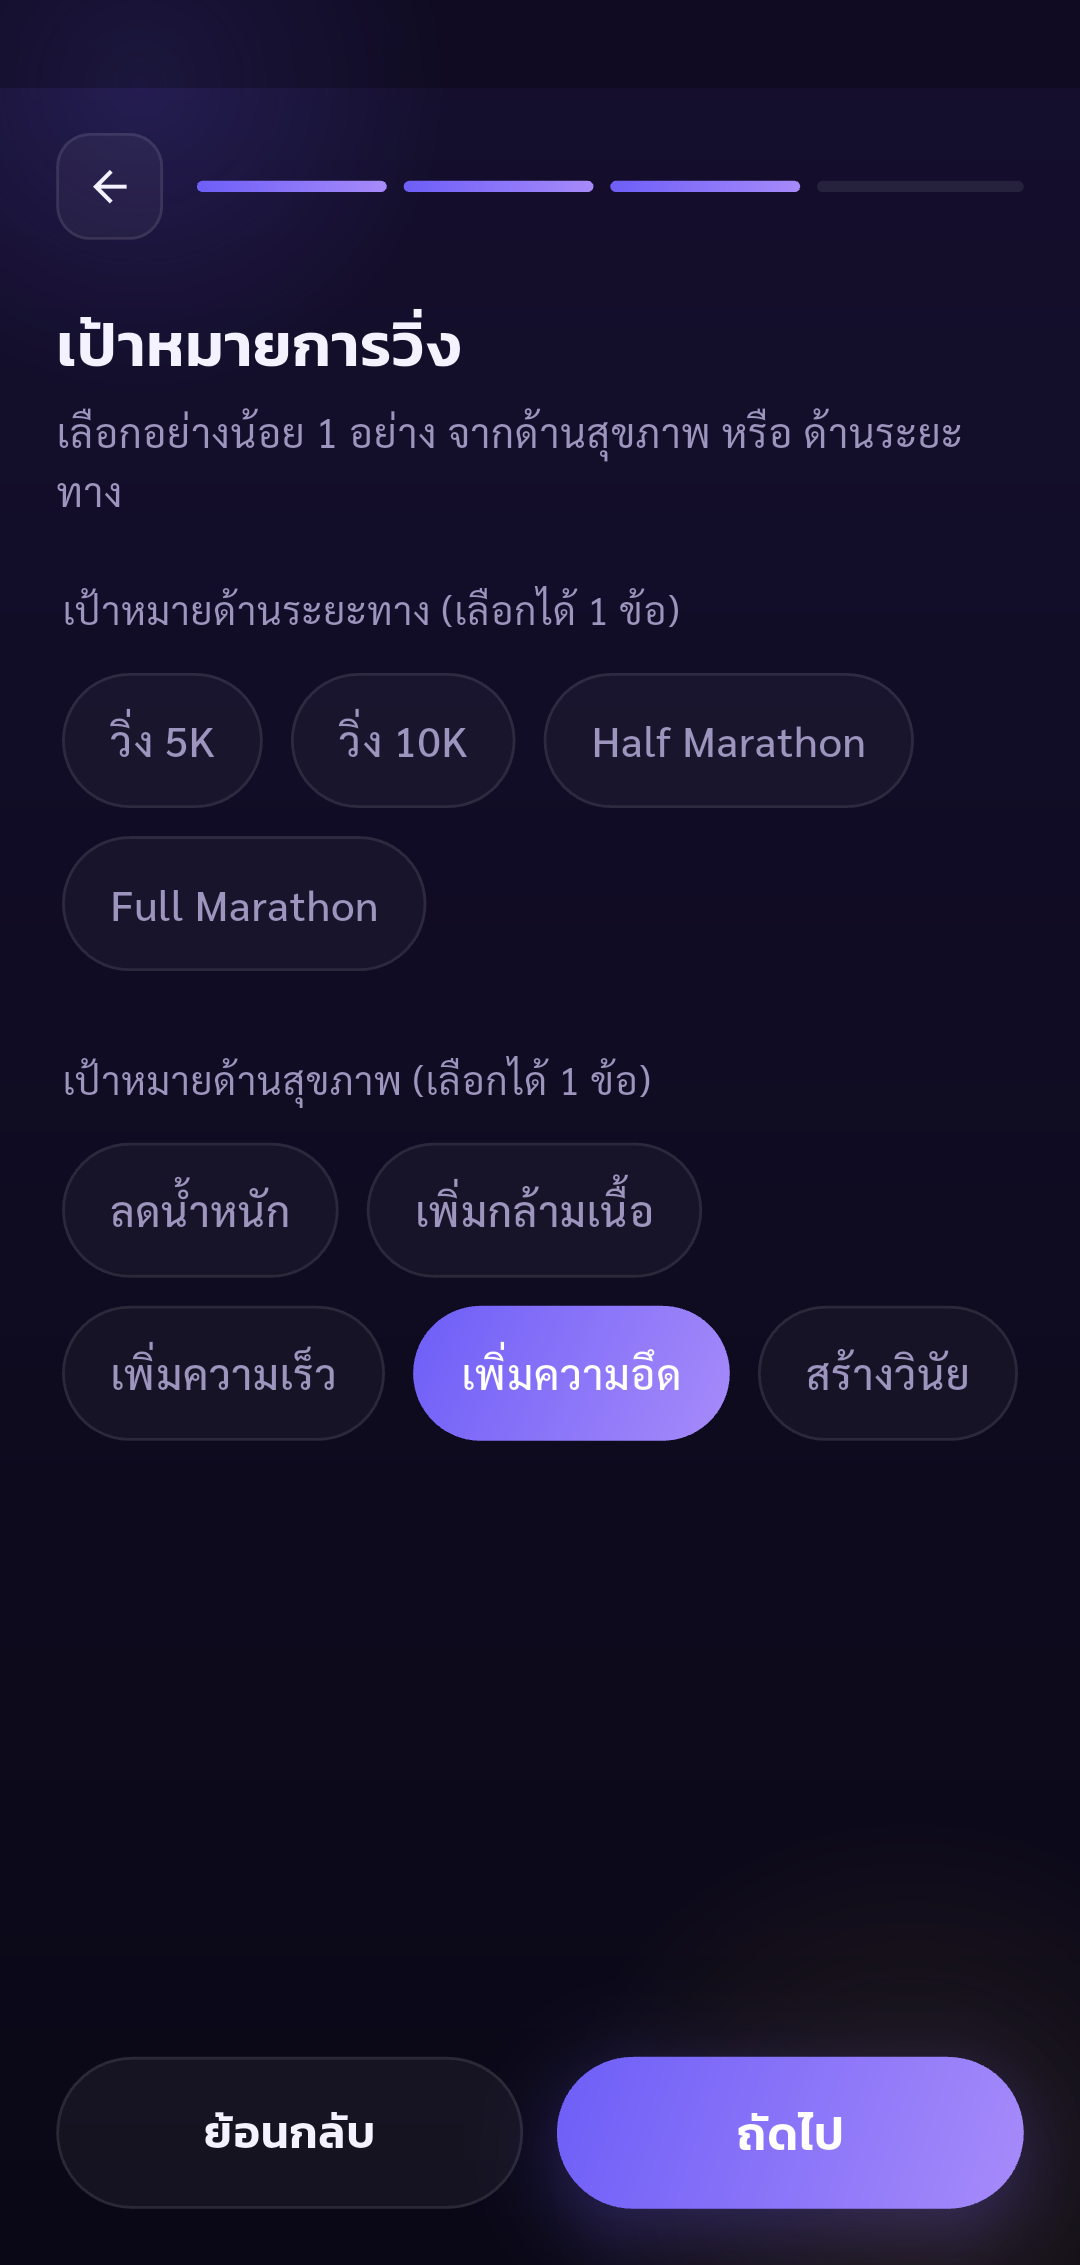
\includegraphics[width=\linewidth,height=0.43\textheight,keepaspectratio]{images/frontend_tests/ft-01-09-09-goal.png}
\caption{เป้าหมายเพิ่มความอึด}\end{subfigure}
\caption{ภาพหลักฐาน FT-01 ชุดที่ 3}\label{fig:flutter-ft-01-3}
\end{figure}

\begin{figure}[H]
\centering
\begin{subfigure}[t]{0.31\textwidth}\centering
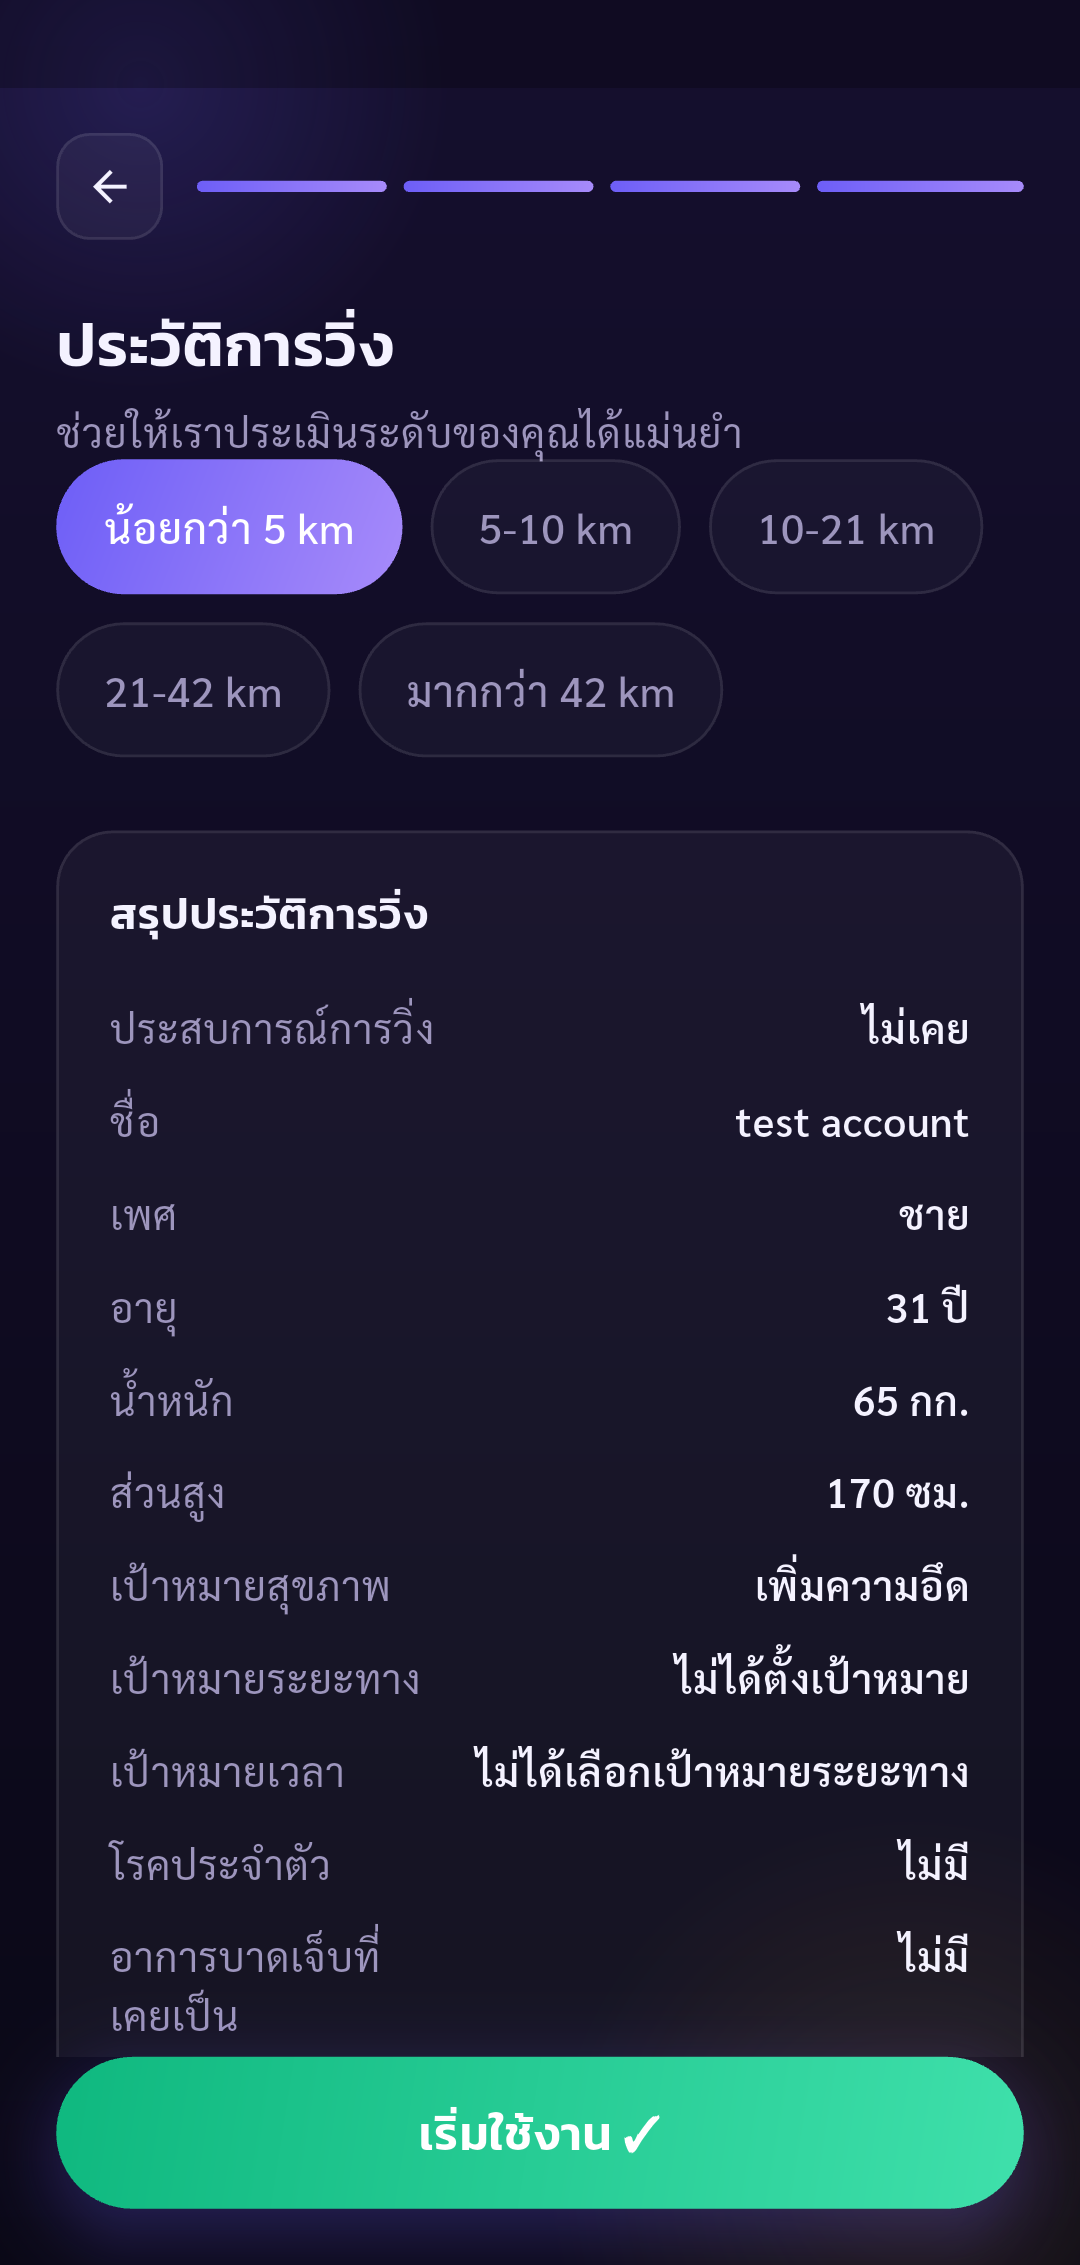
\includegraphics[width=\linewidth,height=0.43\textheight,keepaspectratio]{images/frontend_tests/ft-01-10-10-history.png}
\caption{ประวัติการวิ่ง}\end{subfigure}
\hfill
\begin{subfigure}[t]{0.31\textwidth}\centering

\includegraphics[width=\linewidth,height=0.43\textheight,keepaspectratio]{images/frontend_tests/ft-01-11-11-home.png}
\caption{หน้าหลักหลังกรอกข้อมูล}\end{subfigure}
\hfill
\begin{subfigure}[t]{0.31\textwidth}\centering
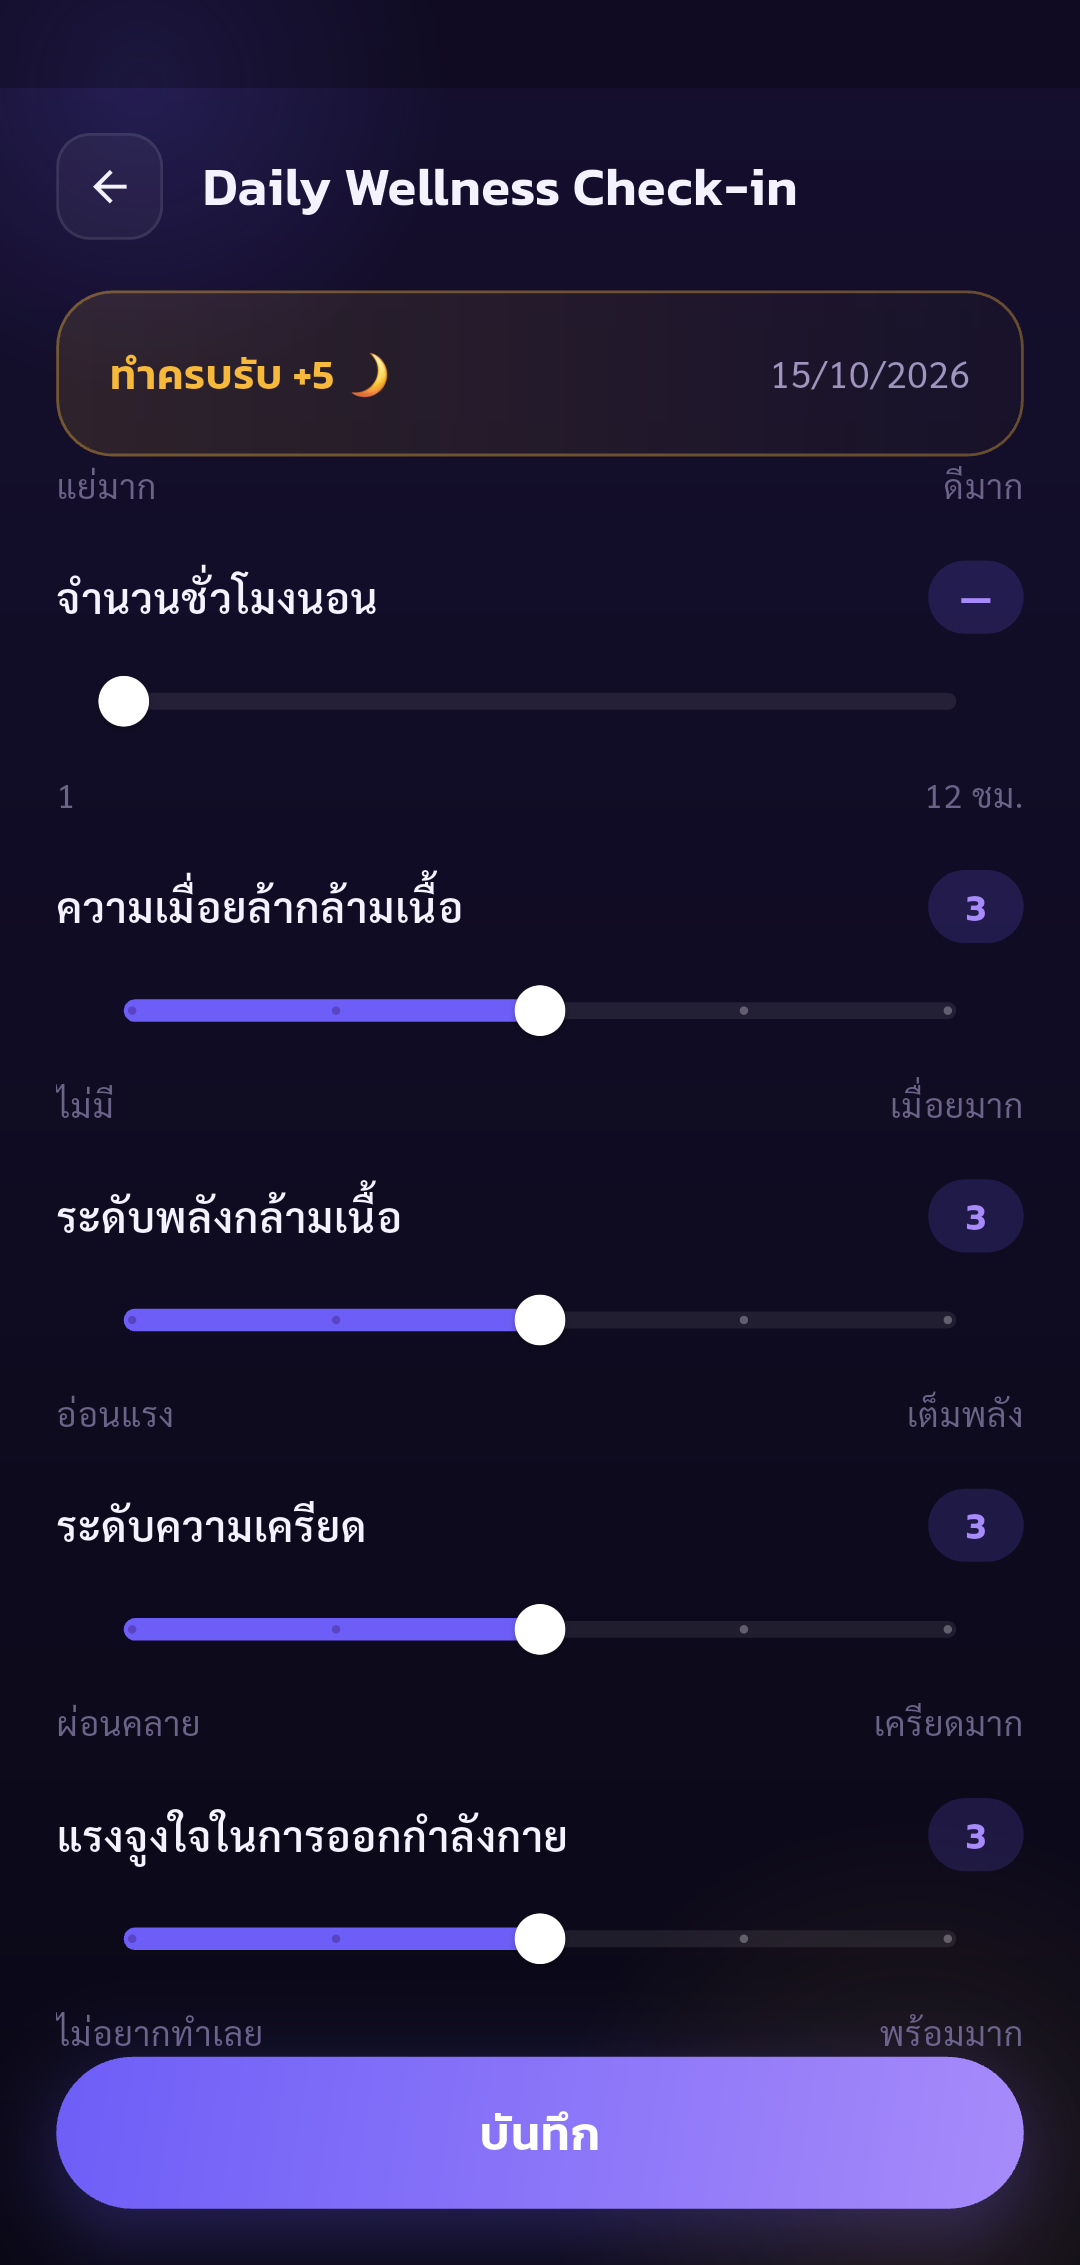
\includegraphics[width=\linewidth,height=0.43\textheight,keepaspectratio]{images/frontend_tests/ft-01-12-12-wellness-valid.png}
\caption{กรอกสุขภาวะครบ}\end{subfigure}
\caption{ภาพหลักฐาน FT-01 ชุดที่ 4}\label{fig:flutter-ft-01-4}
\end{figure}

\begin{figure}[H]
\centering
\begin{subfigure}[t]{0.31\textwidth}\centering

\includegraphics[width=\linewidth,height=0.43\textheight,keepaspectratio]{images/frontend_tests/ft-01-13-13-wellness-saved.png}
\caption{บันทึกสุขภาวะ}\end{subfigure}
\hfill
\begin{subfigure}[t]{0.31\textwidth}\centering
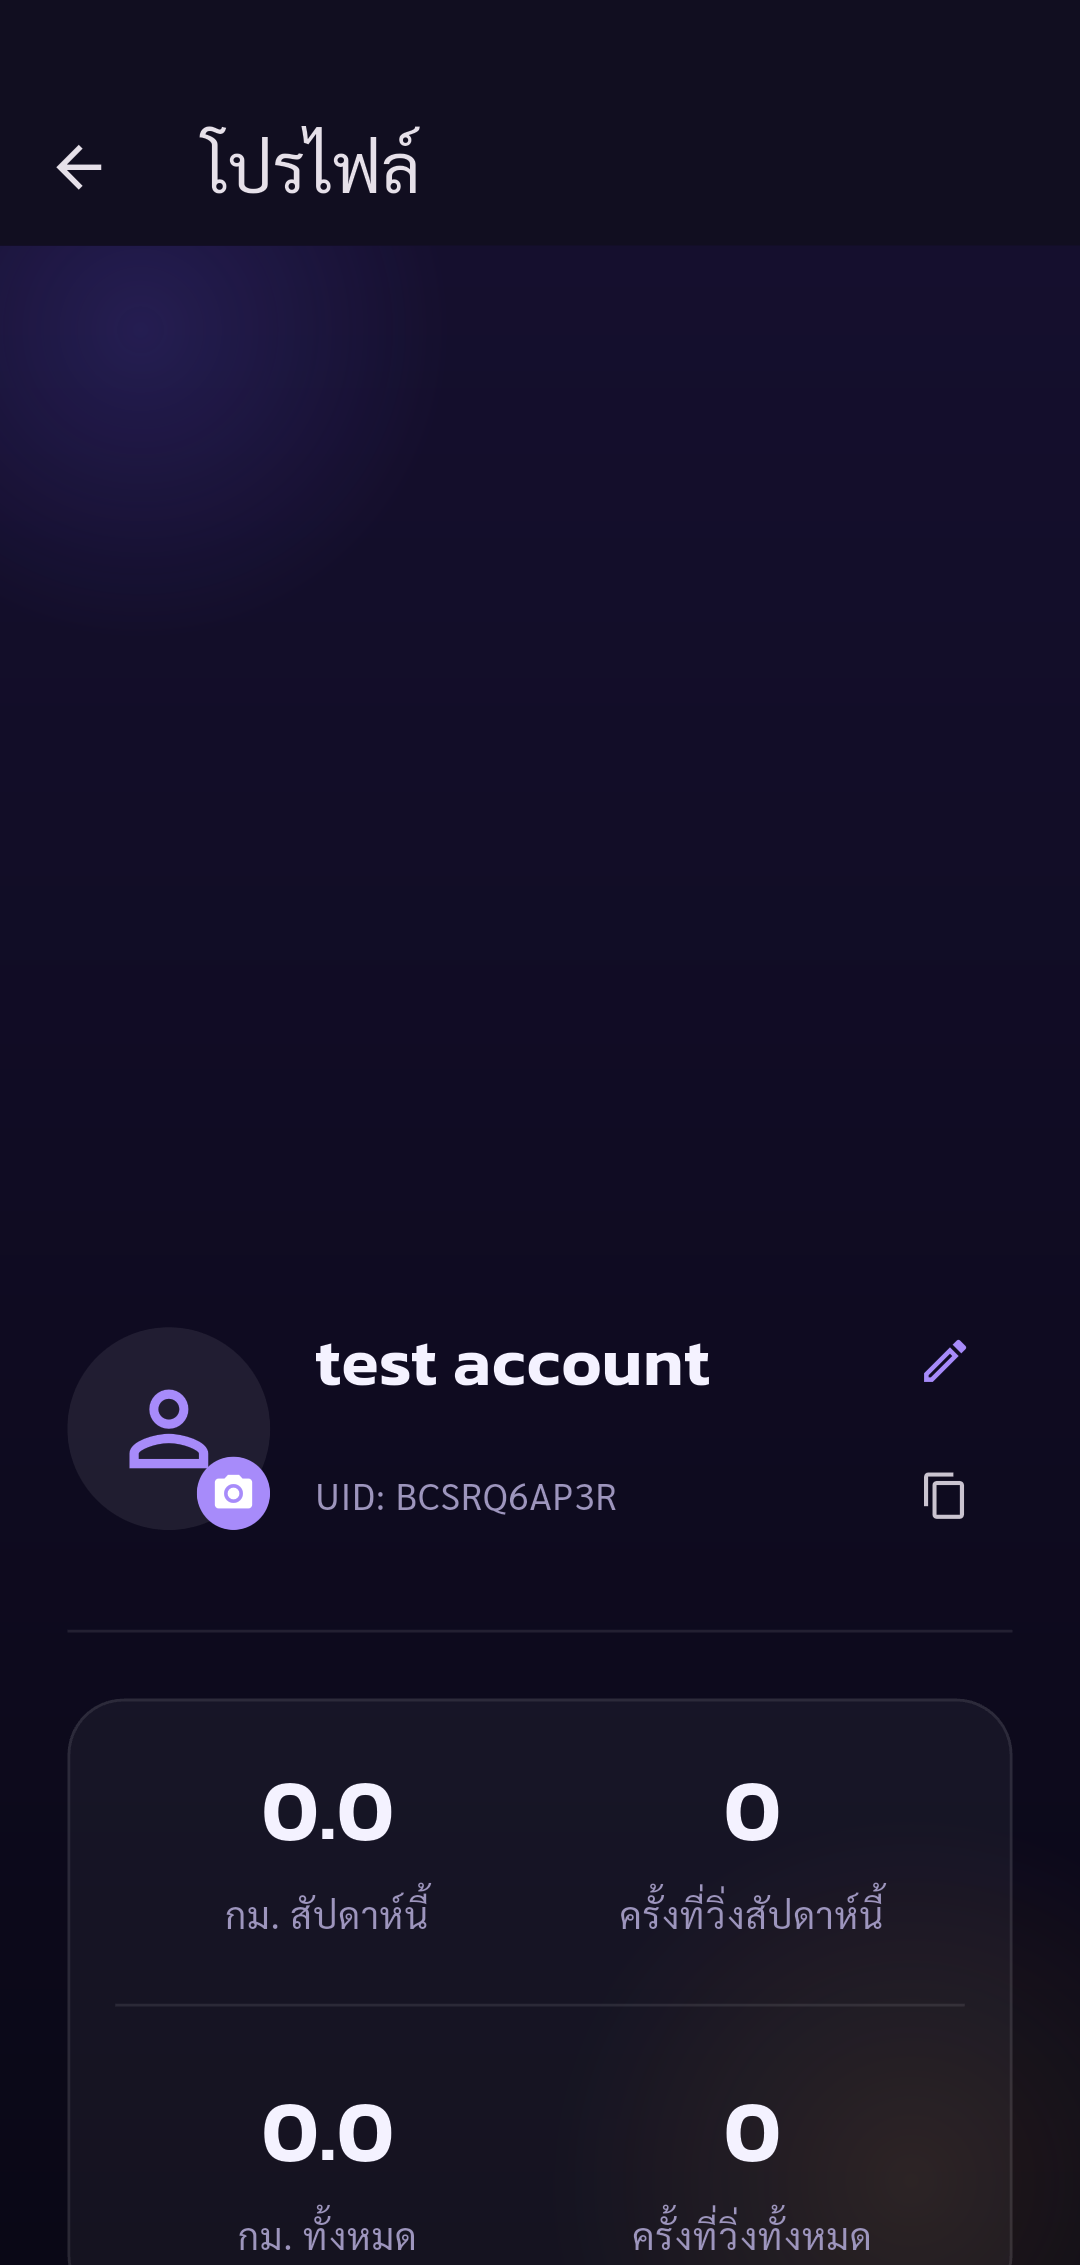
\includegraphics[width=\linewidth,height=0.43\textheight,keepaspectratio]{images/frontend_tests/ft-01-14-14-profile.png}
\caption{โปรไฟล์บัญชีทดสอบ}\end{subfigure}
\caption{ภาพหลักฐาน FT-01 ชุดที่ 5}\label{fig:flutter-ft-01-5}
\end{figure}

\subsubsection{FT-02 โปรแกรมและตารางฝึกซ้อม}

รอบนี้ใช้โปรแกรมที่สมัครค้างไว้และกลับมาจัดตาราง จึงยืนยันการวางและบันทึกตารางตามที่ตรวจได้ โดยไม่ได้ยืนยันกระบวนการสมัครโปรแกรมใหม่ครบทุกขั้นตอน

\begingroup
\small
\renewcommand{\arraystretch}{1.15}
\begin{longtable}{|>{\raggedright\arraybackslash}p{0.07\textwidth}|>{\raggedright\arraybackslash}p{0.57\textwidth}|>{\raggedright\arraybackslash}p{0.08\textwidth}|>{\raggedright\arraybackslash}p{0.16\textwidth}|}
\caption{ผลการทดสอบ FT-02}\label{tab:flutter-ft-02}\\ \hline
\textbf{ลำดับ} & \textbf{จุดตรวจและผลที่ได้รับจริง} & \textbf{ผล} & \textbf{หลักฐาน} \\ \hline
\endfirsthead
\multicolumn{4}{c}{ผลการทดสอบ FT-02 (ต่อ)} \\ \hline
\textbf{ลำดับ} & \textbf{จุดตรวจและผลที่ได้รับจริง} & \textbf{ผล} & \textbf{หลักฐาน} \\ \hline
\endhead
\endfoot
\endlastfoot
1 & สัปดาห์ใหม่ยังบันทึกไม่ได้ก่อนวางกิจกรรมฝึกครบตามข้อกำหนด & ผ่าน & ภาพที่~\ref{fig:flutter-ft-02-1} (a) \\ \hline
2 & วาง Easy Run ครบ 3 วันแล้วตัวเลือกถูกนำออก และการแตะวันว่างไม่เพิ่ม Easy Run วันที่ 4 & ผ่าน & ภาพที่~\ref{fig:flutter-ft-02-1} (b) \\ \hline
3 & วาง Easy Run วันที่ 1, 3 และ 5 และ Long Run วันที่ 7 แล้วปุ่มบันทึกใช้งานได้ & ผ่าน & ภาพที่~\ref{fig:flutter-ft-02-1} (c) \\ \hline
4 & กลับมาจัดตารางของโปรแกรมที่สมัครค้างไว้และบันทึกภารกิจ 4 รายการ ได้แก่ Easy Run 3 รายการและ Long Run 1 รายการ (ตรวจบางส่วนของ SFT-02-008 และ SFT-02-010) & ผ่าน & ภาพที่~\ref{fig:flutter-ft-02-2} (a) \\ \hline
5 & เปิดตารางใหม่แล้วตำแหน่งวันตรงกับที่บันทึก และ API ยังคงมีภารกิจ 4 รายการ & ผ่าน & ภาพที่~\ref{fig:flutter-ft-02-2} (b) \\ \hline
\end{longtable}
\endgroup

\begin{figure}[H]
\centering
\begin{subfigure}[t]{0.31\textwidth}\centering
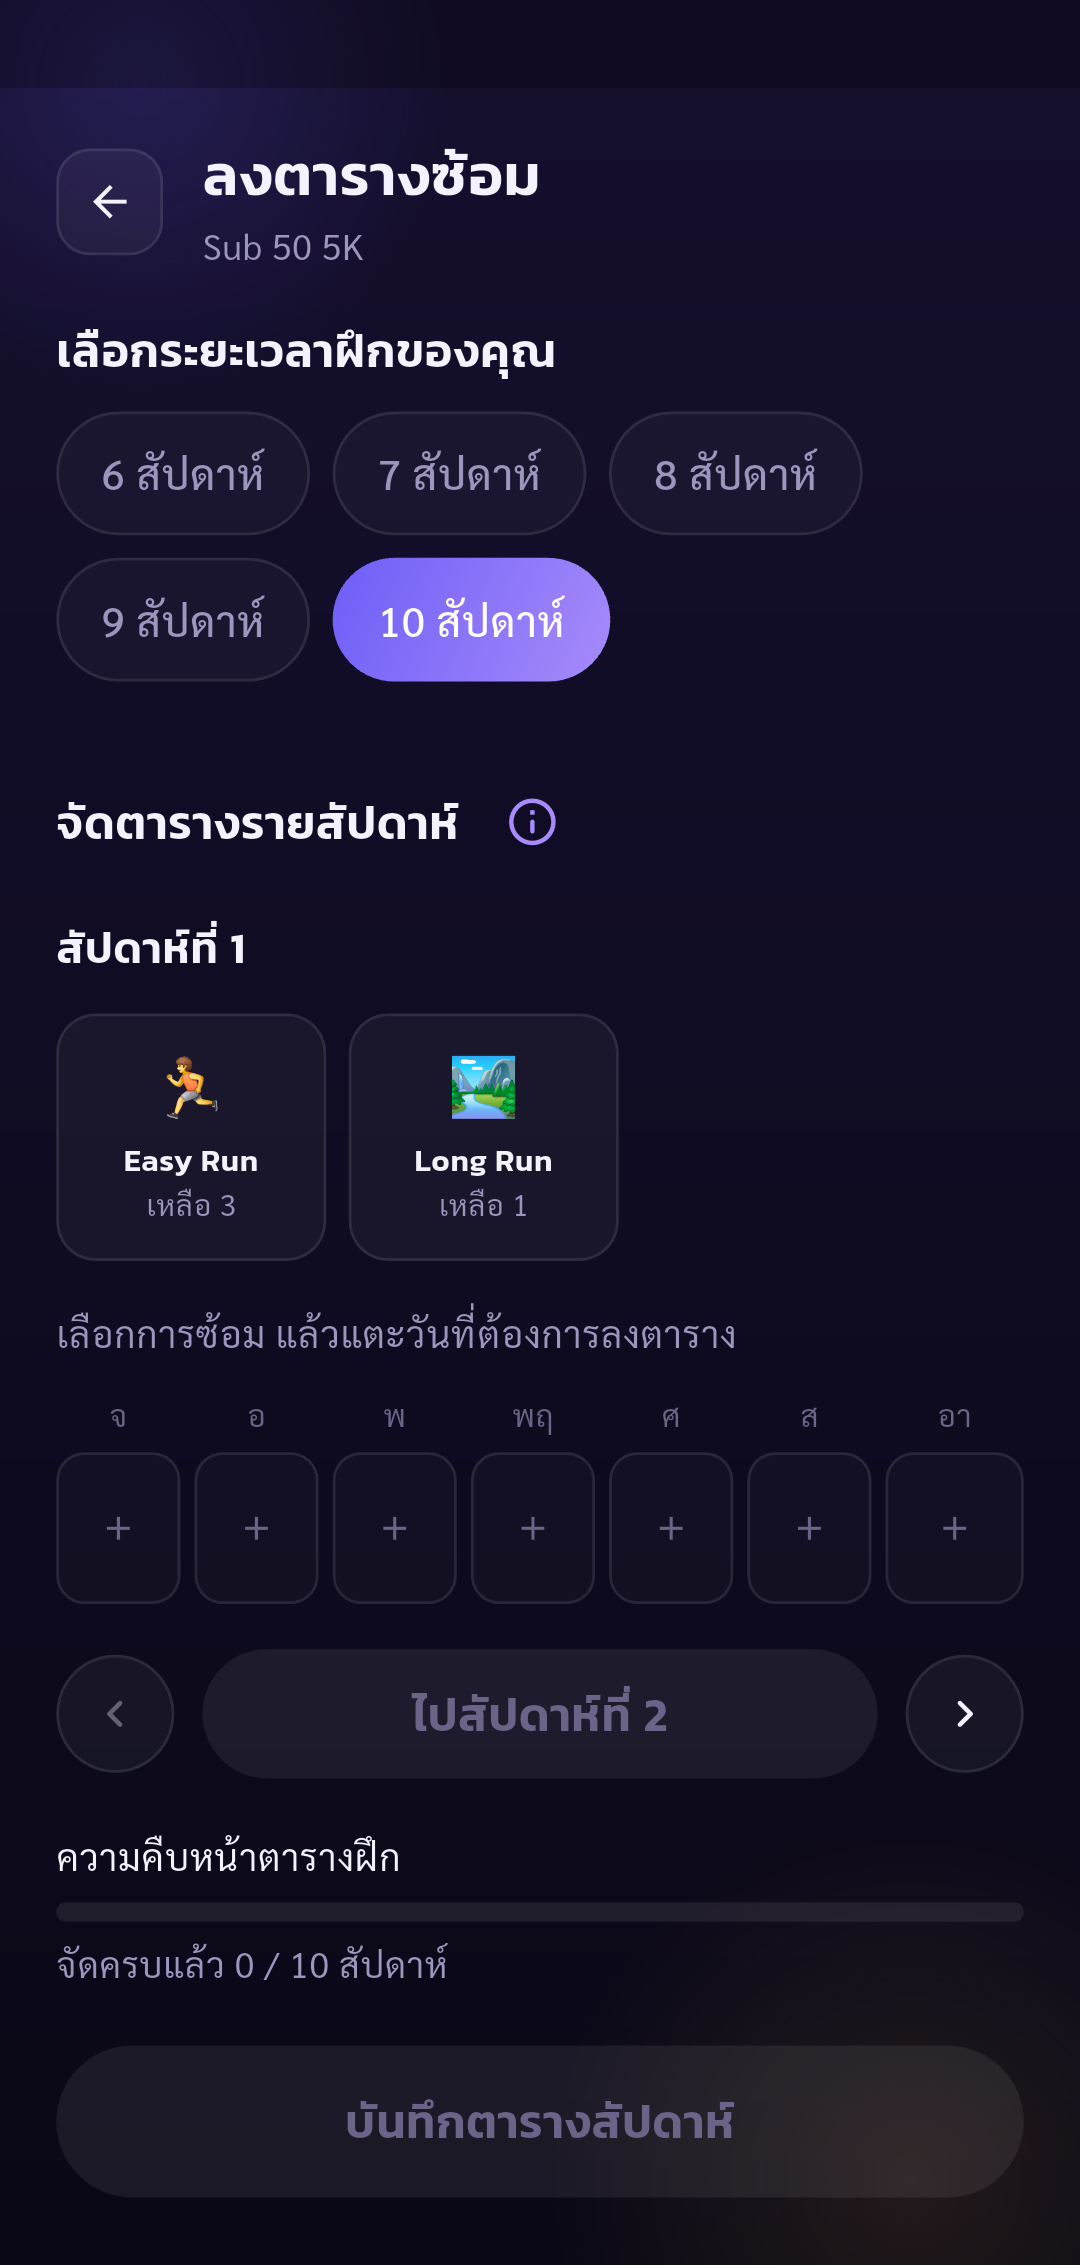
\includegraphics[width=\linewidth,height=0.43\textheight,keepaspectratio]{images/frontend_tests/ft-02-01-schedule-incomplete.png}
\caption{ตารางยังไม่ครบ}\end{subfigure}
\hfill
\begin{subfigure}[t]{0.31\textwidth}\centering
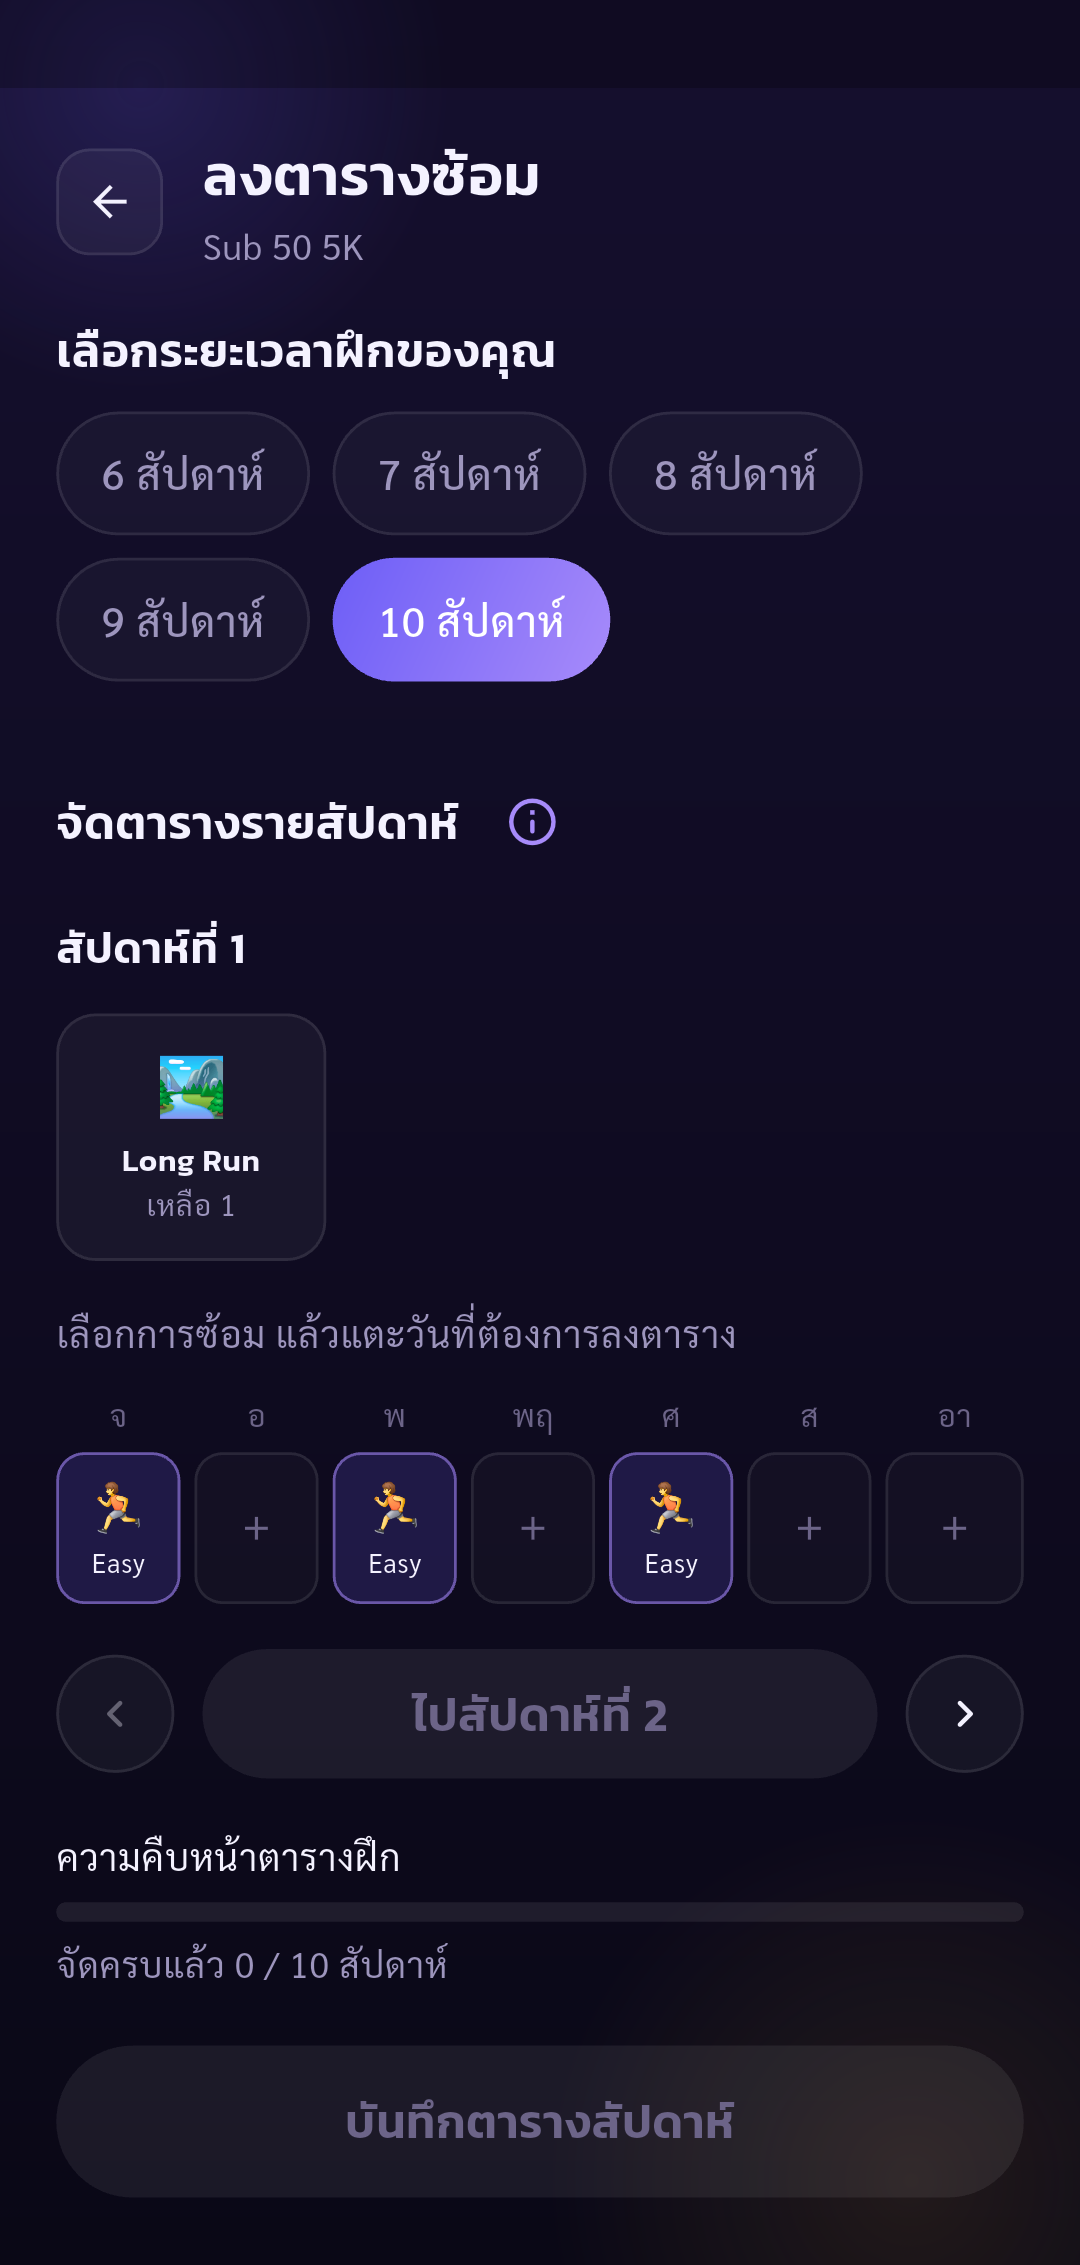
\includegraphics[width=\linewidth,height=0.43\textheight,keepaspectratio]{images/frontend_tests/ft-02-02-schedule-quota.png}
\caption{ครบโควตา Easy Run}\end{subfigure}
\hfill
\begin{subfigure}[t]{0.31\textwidth}\centering
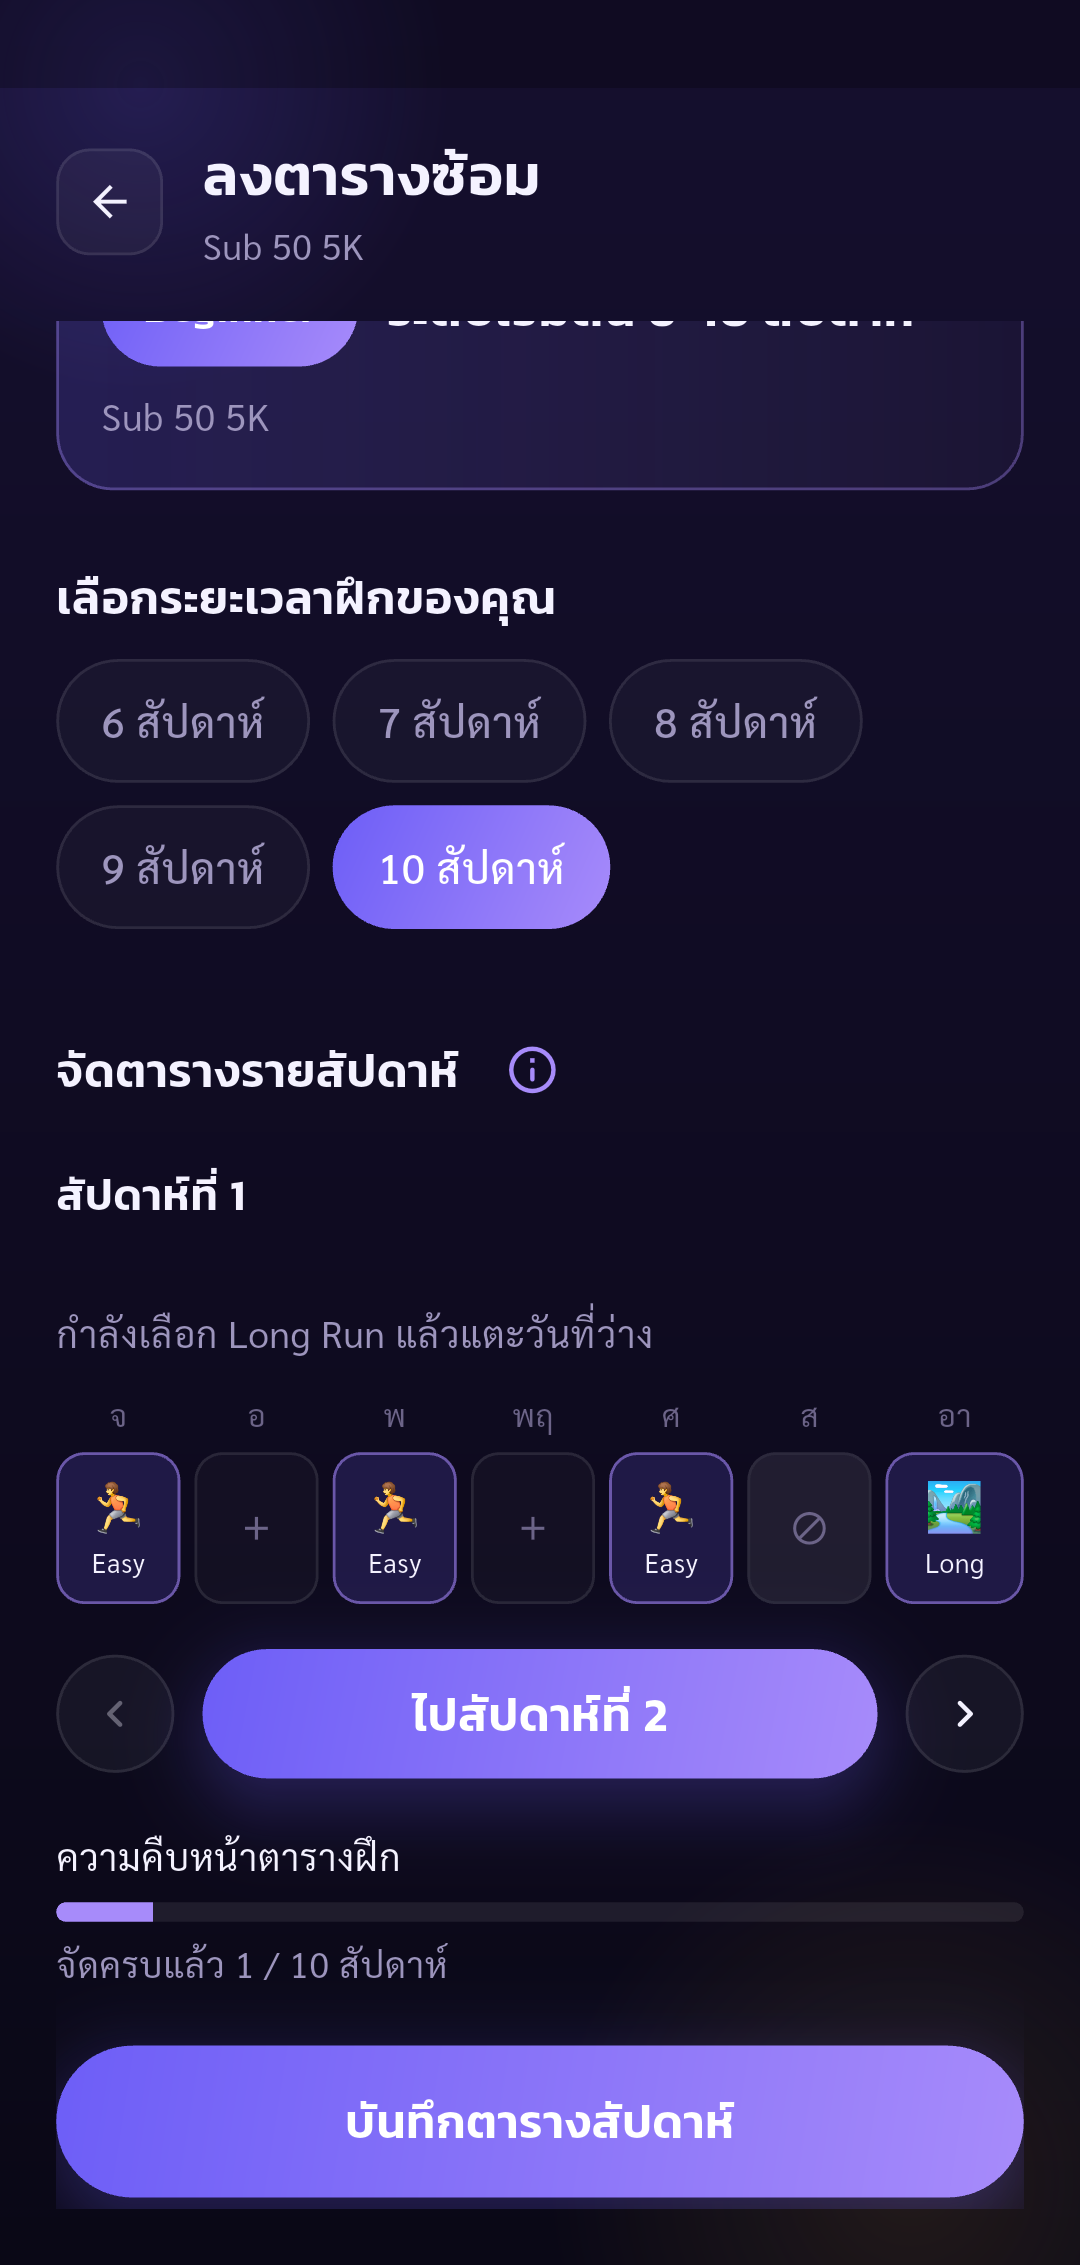
\includegraphics[width=\linewidth,height=0.43\textheight,keepaspectratio]{images/frontend_tests/ft-02-03-schedule-ready.png}
\caption{ตารางพร้อมบันทึก}\end{subfigure}
\caption{ภาพหลักฐาน FT-02 ชุดที่ 1}\label{fig:flutter-ft-02-1}
\end{figure}

\begin{figure}[H]
\centering
\begin{subfigure}[t]{0.31\textwidth}\centering
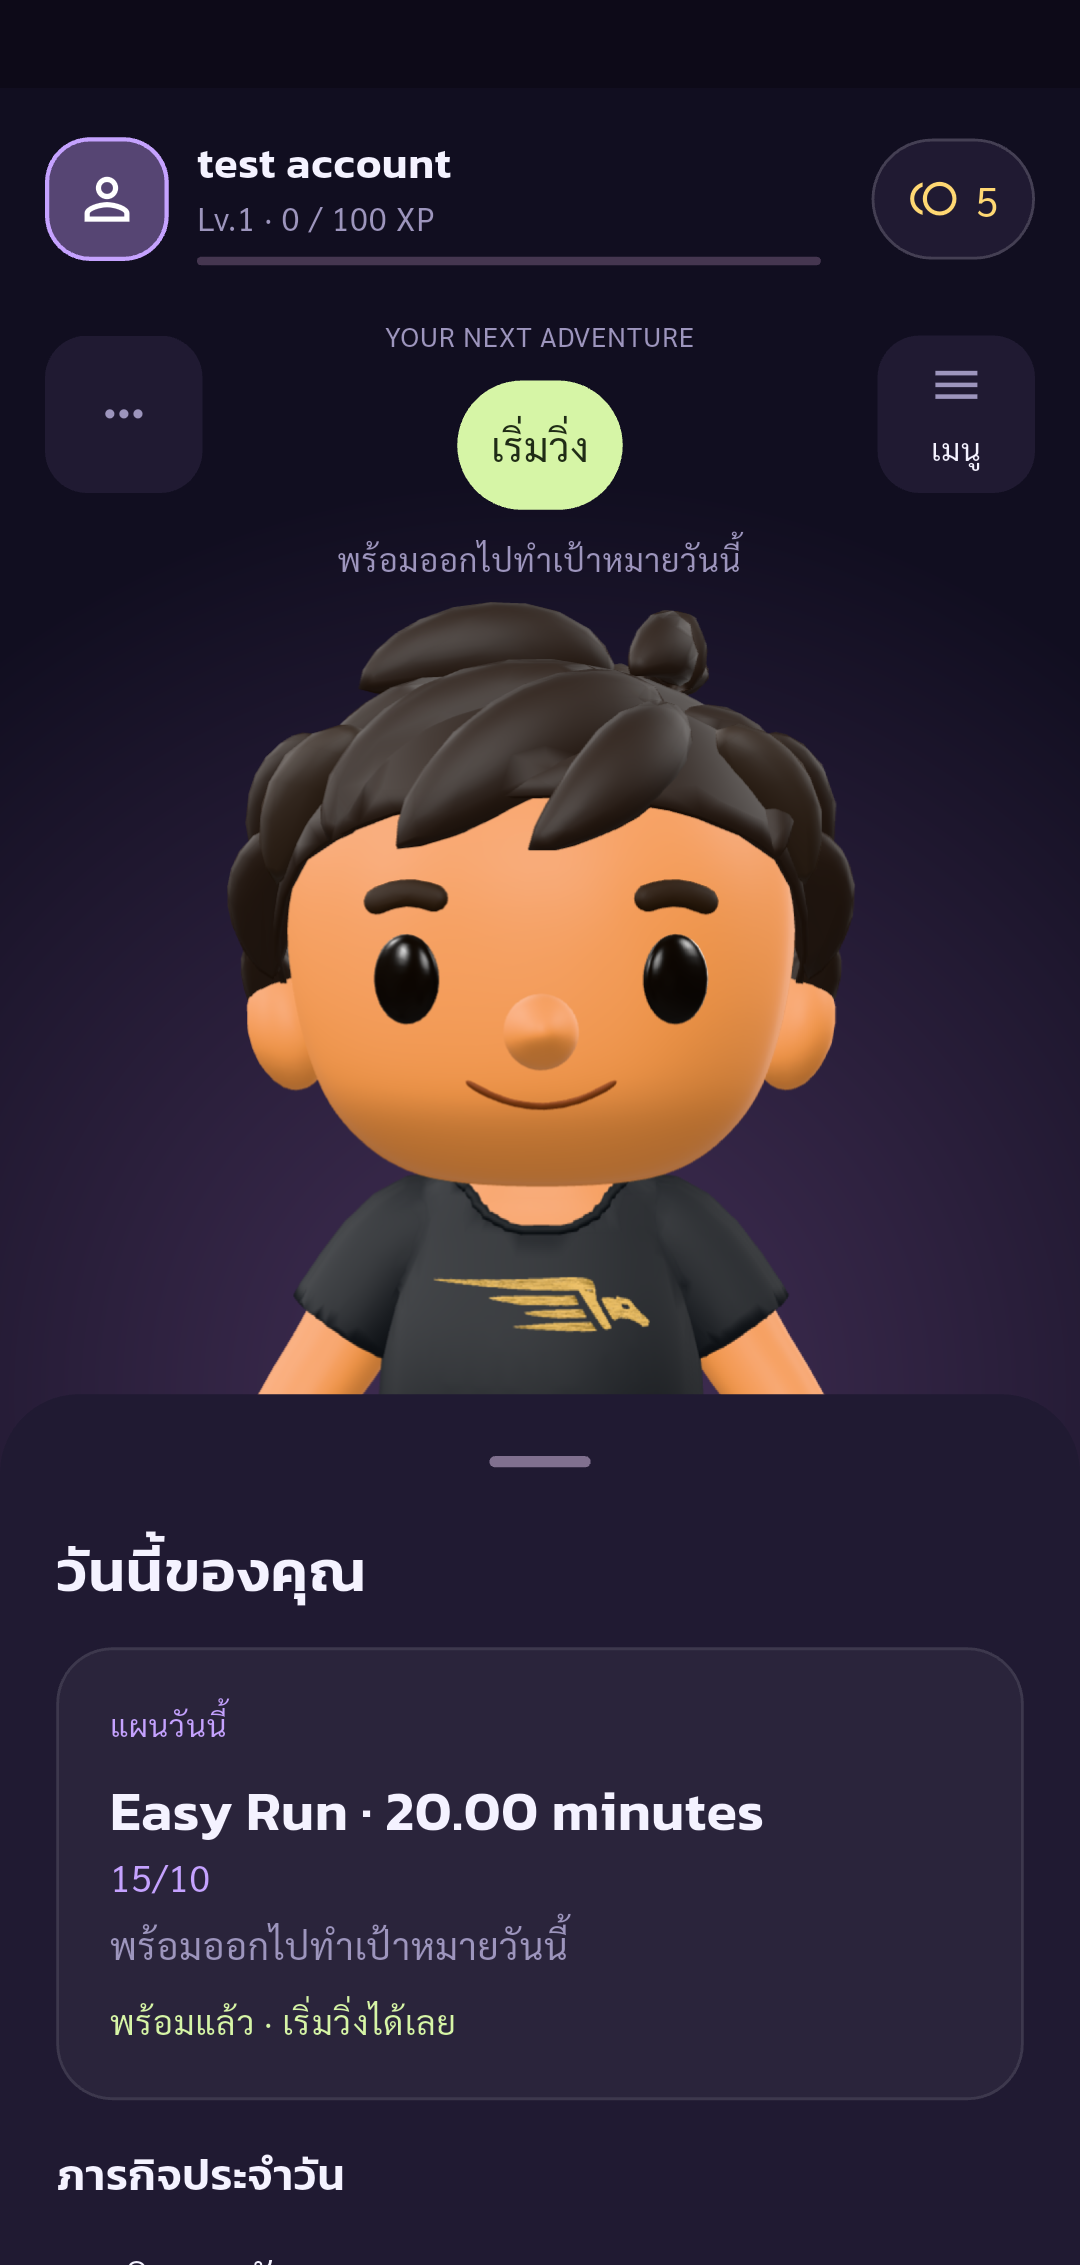
\includegraphics[width=\linewidth,height=0.43\textheight,keepaspectratio]{images/frontend_tests/ft-02-04-program-saved.png}
\caption{บันทึกโปรแกรม}\end{subfigure}
\hfill
\begin{subfigure}[t]{0.31\textwidth}\centering
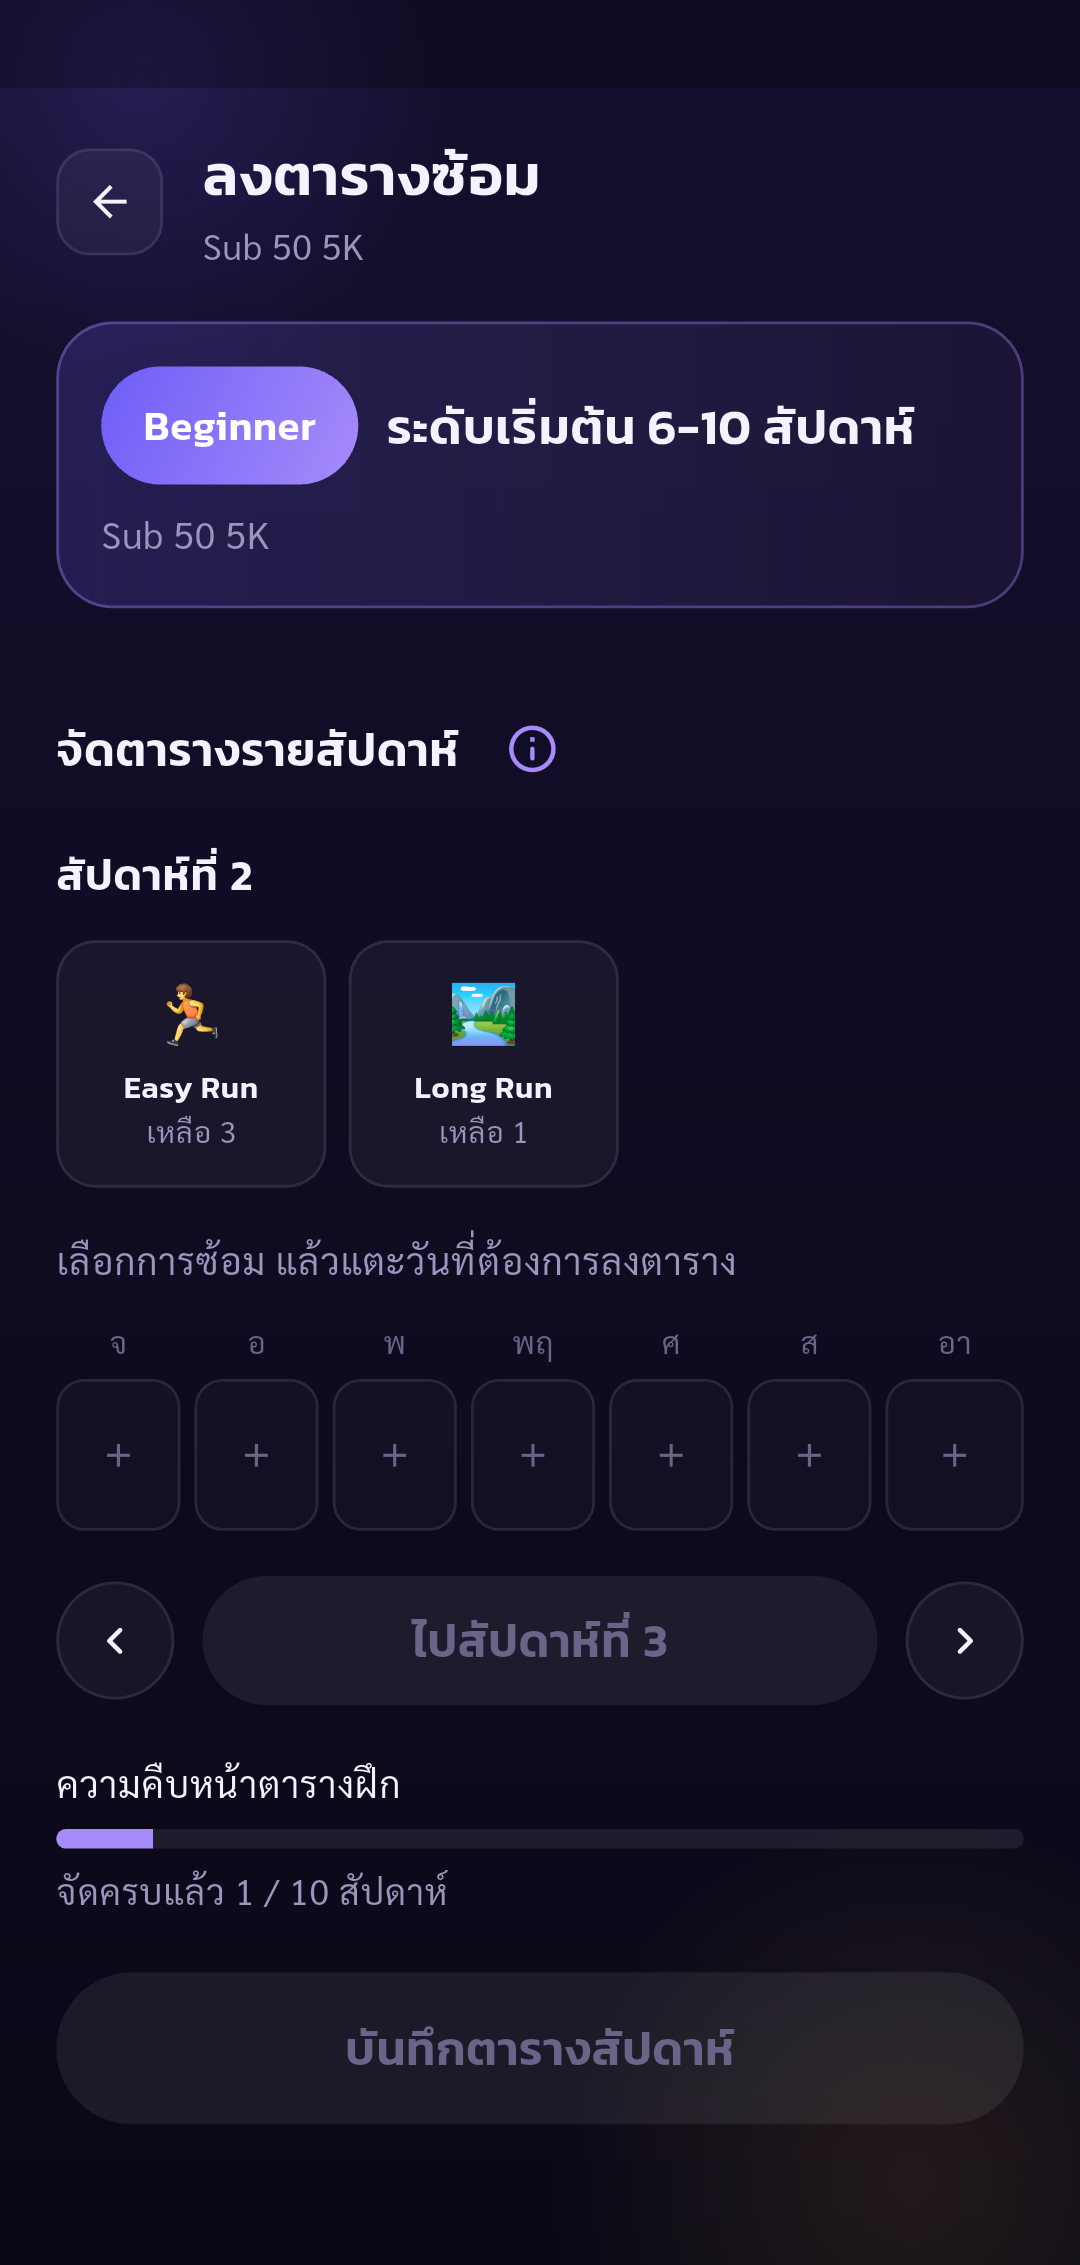
\includegraphics[width=\linewidth,height=0.43\textheight,keepaspectratio]{images/frontend_tests/ft-02-05-schedule-restored.png}
\caption{เปิดตารางตรวจซ้ำ}\end{subfigure}
\caption{ภาพหลักฐาน FT-02 ชุดที่ 2}\label{fig:flutter-ft-02-2}
\end{figure}

\subsubsection{FT-03 วิ่งในลู่และ Park สรุปผล รางวัล สถิติ และประวัติ}

ภาพและผลมาจากรอบวิ่งในลู่ รอบสวนสาธารณะ และการตรวจประวัติ ซึ่งเป็นคนละเซสชัน ระยะลู่ 0.10 km เป็นค่ากรอกทดสอบ ส่วน Park ได้ตำแหน่ง GPS จริงขณะอุปกรณ์อยู่กับที่ ระยะ 0.00 km

\begingroup
\small
\renewcommand{\arraystretch}{1.15}
\begin{longtable}{|>{\raggedright\arraybackslash}p{0.07\textwidth}|>{\raggedright\arraybackslash}p{0.57\textwidth}|>{\raggedright\arraybackslash}p{0.08\textwidth}|>{\raggedright\arraybackslash}p{0.16\textwidth}|}
\caption{ผลการทดสอบ FT-03}\label{tab:flutter-ft-03}\\ \hline
\textbf{ลำดับ} & \textbf{จุดตรวจและผลที่ได้รับจริง} & \textbf{ผล} & \textbf{หลักฐาน} \\ \hline
\endfirsthead
\multicolumn{4}{c}{ผลการทดสอบ FT-03 (ต่อ)} \\ \hline
\textbf{ลำดับ} & \textbf{จุดตรวจและผลที่ได้รับจริง} & \textbf{ผล} & \textbf{หลักฐาน} \\ \hline
\endhead
\endfoot
\endlastfoot
1 & เปิดหน้าวิ่งและเลือกสภาพแวดล้อมเป็นลู่ก่อนเริ่ม & ผ่าน & ภาพที่~\ref{fig:flutter-ft-03-1} (a) \\ \hline
2 & เริ่มเซสชันวิ่งในลู่ได้จริง พักแล้วเวลาไม่เพิ่มตลอดช่วงตรวจ 3 วินาที และทำต่อได้ & ผ่าน & ภาพที่~\ref{fig:flutter-ft-03-1} (b) \\ \hline
3 & จบวิ่งในลู่แล้วหน้าสรุปแสดงระยะกรอกทดสอบ 0.10 km และส่งข้อมูลประเมินหลังวิ่งได้เมื่อกรอกครบ & ผ่าน & ภาพที่~\ref{fig:flutter-ft-03-1} (c) \\ \hline
4 & เปิดหน้าวิ่ง Park และโหลดรายการก่อนเริ่มได้ & ผ่าน & ภาพที่~\ref{fig:flutter-ft-03-2} (a) \\ \hline
5 & ระหว่างวิ่ง Park ได้รับตำแหน่ง GPS จริงและรออย่างน้อย 5 วินาทีก่อนจบ & ผ่าน & ภาพที่~\ref{fig:flutter-ft-03-2} (b) \\ \hline
6 & จบวิ่ง Park แล้วแสดงสรุปและบันทึกข้อมูลประเมินหลังวิ่งได้ ระยะ 0.00 km ขณะอุปกรณ์อยู่กับที่ & ผ่าน & ภาพที่~\ref{fig:flutter-ft-03-2} (c) \\ \hline
7 & หน้ารับรางวัลหลังจบ Park แสดง 5 เหรียญ ตรงกับยอดที่เพิ่มจริง & ผ่าน & ภาพที่~\ref{fig:flutter-ft-03-3} (a) \\ \hline
8 & ตรวจสถิติและประวัติพบเซสชันใหม่หนึ่งรายการ และยอดสถิติตรงกับประวัติจริง & ผ่าน & ภาพที่~\ref{fig:flutter-ft-03-3} (b) \\ \hline
9 & เปิดรายละเอียดเซสชัน Park ที่บันทึกไว้และรอโหลดข้อมูลจริงสำเร็จ & ผ่าน & ภาพที่~\ref{fig:flutter-ft-03-3} (c) \\ \hline
\end{longtable}
\endgroup

\begin{figure}[H]
\centering
\begin{subfigure}[t]{0.31\textwidth}\centering
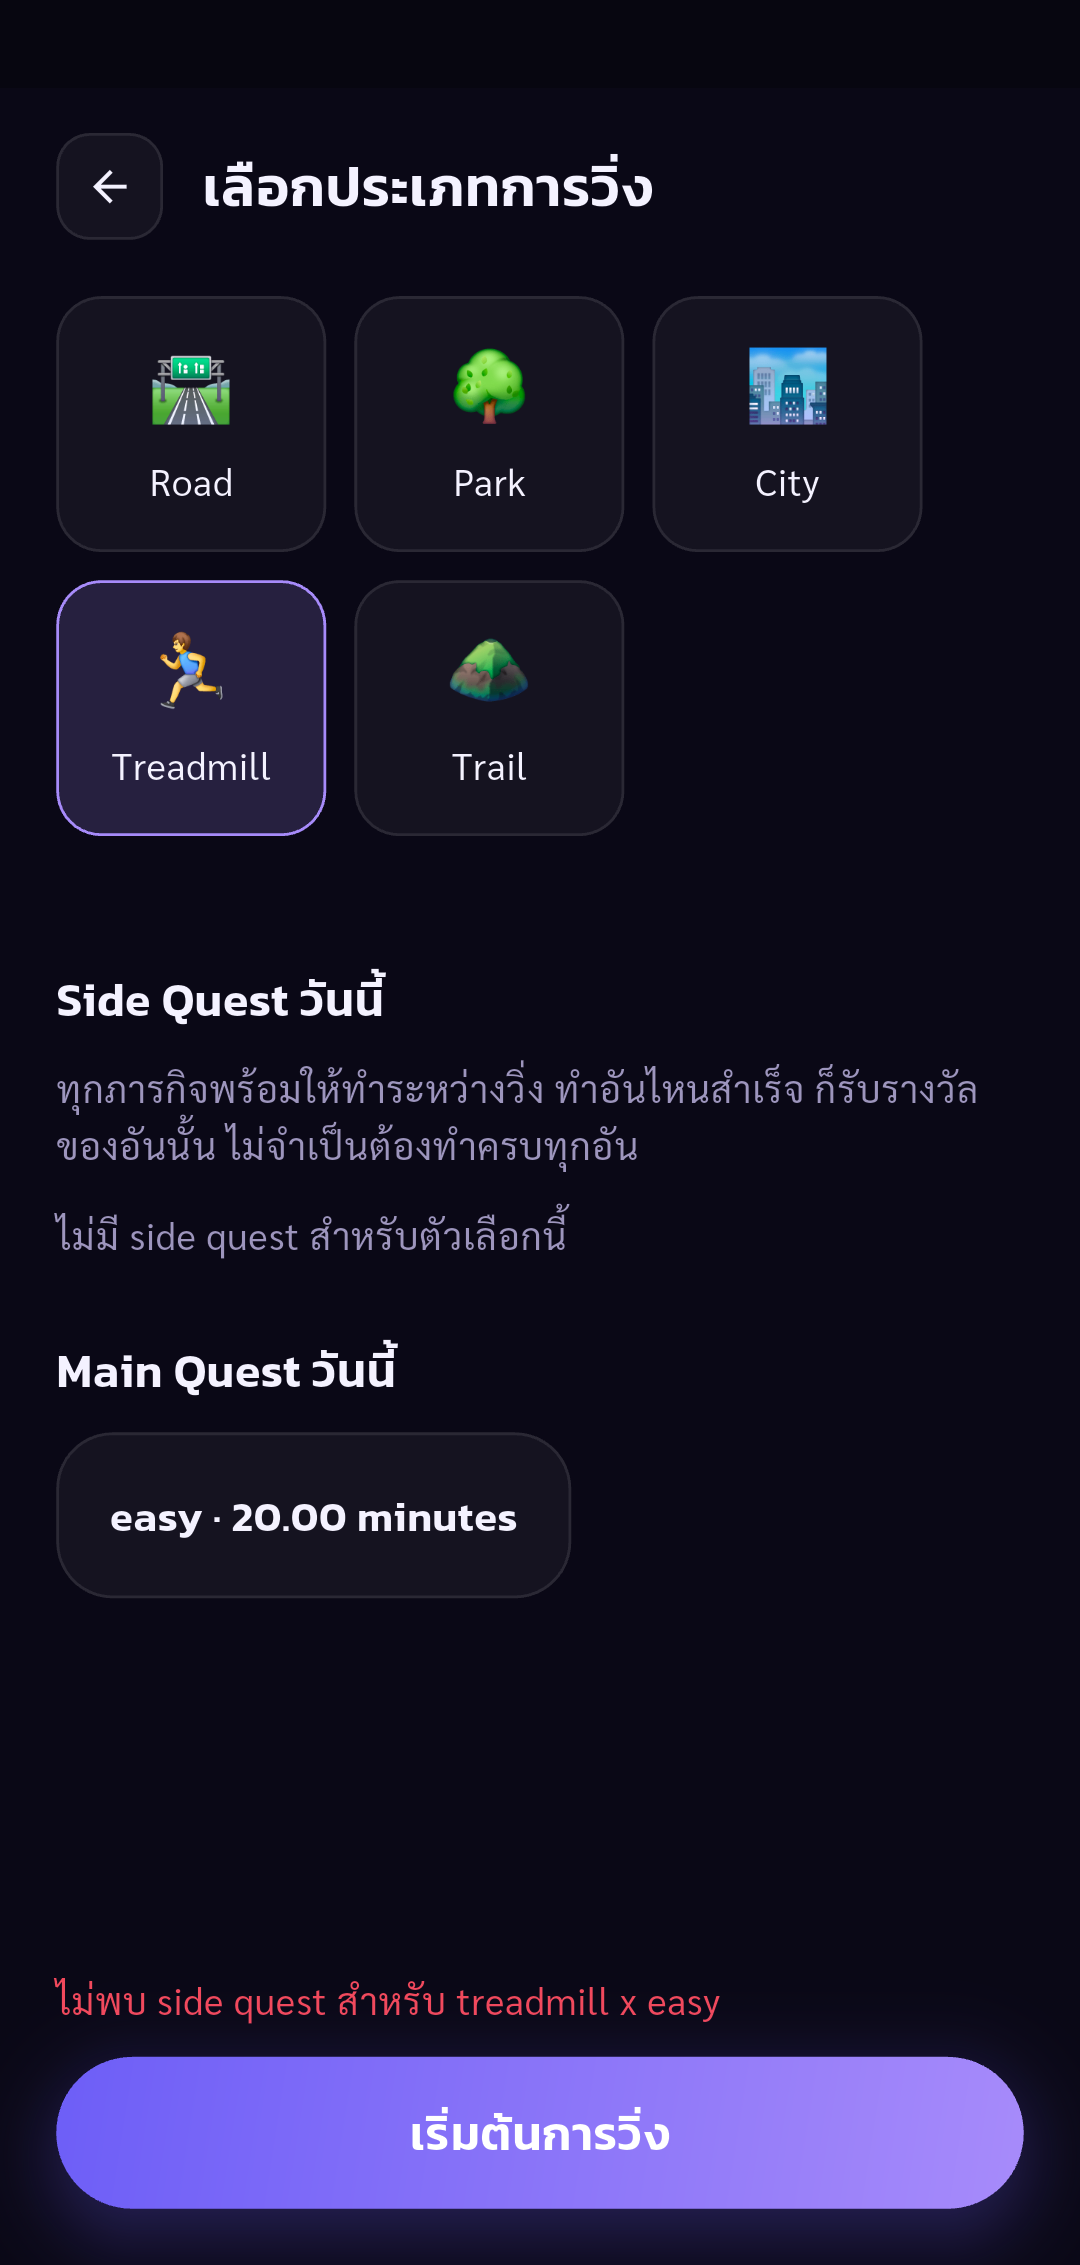
\includegraphics[width=\linewidth,height=0.43\textheight,keepaspectratio]{images/frontend_tests/ft-03-01-run-environment.png}
\caption{เลือกวิ่งในลู่}\end{subfigure}
\hfill
\begin{subfigure}[t]{0.31\textwidth}\centering
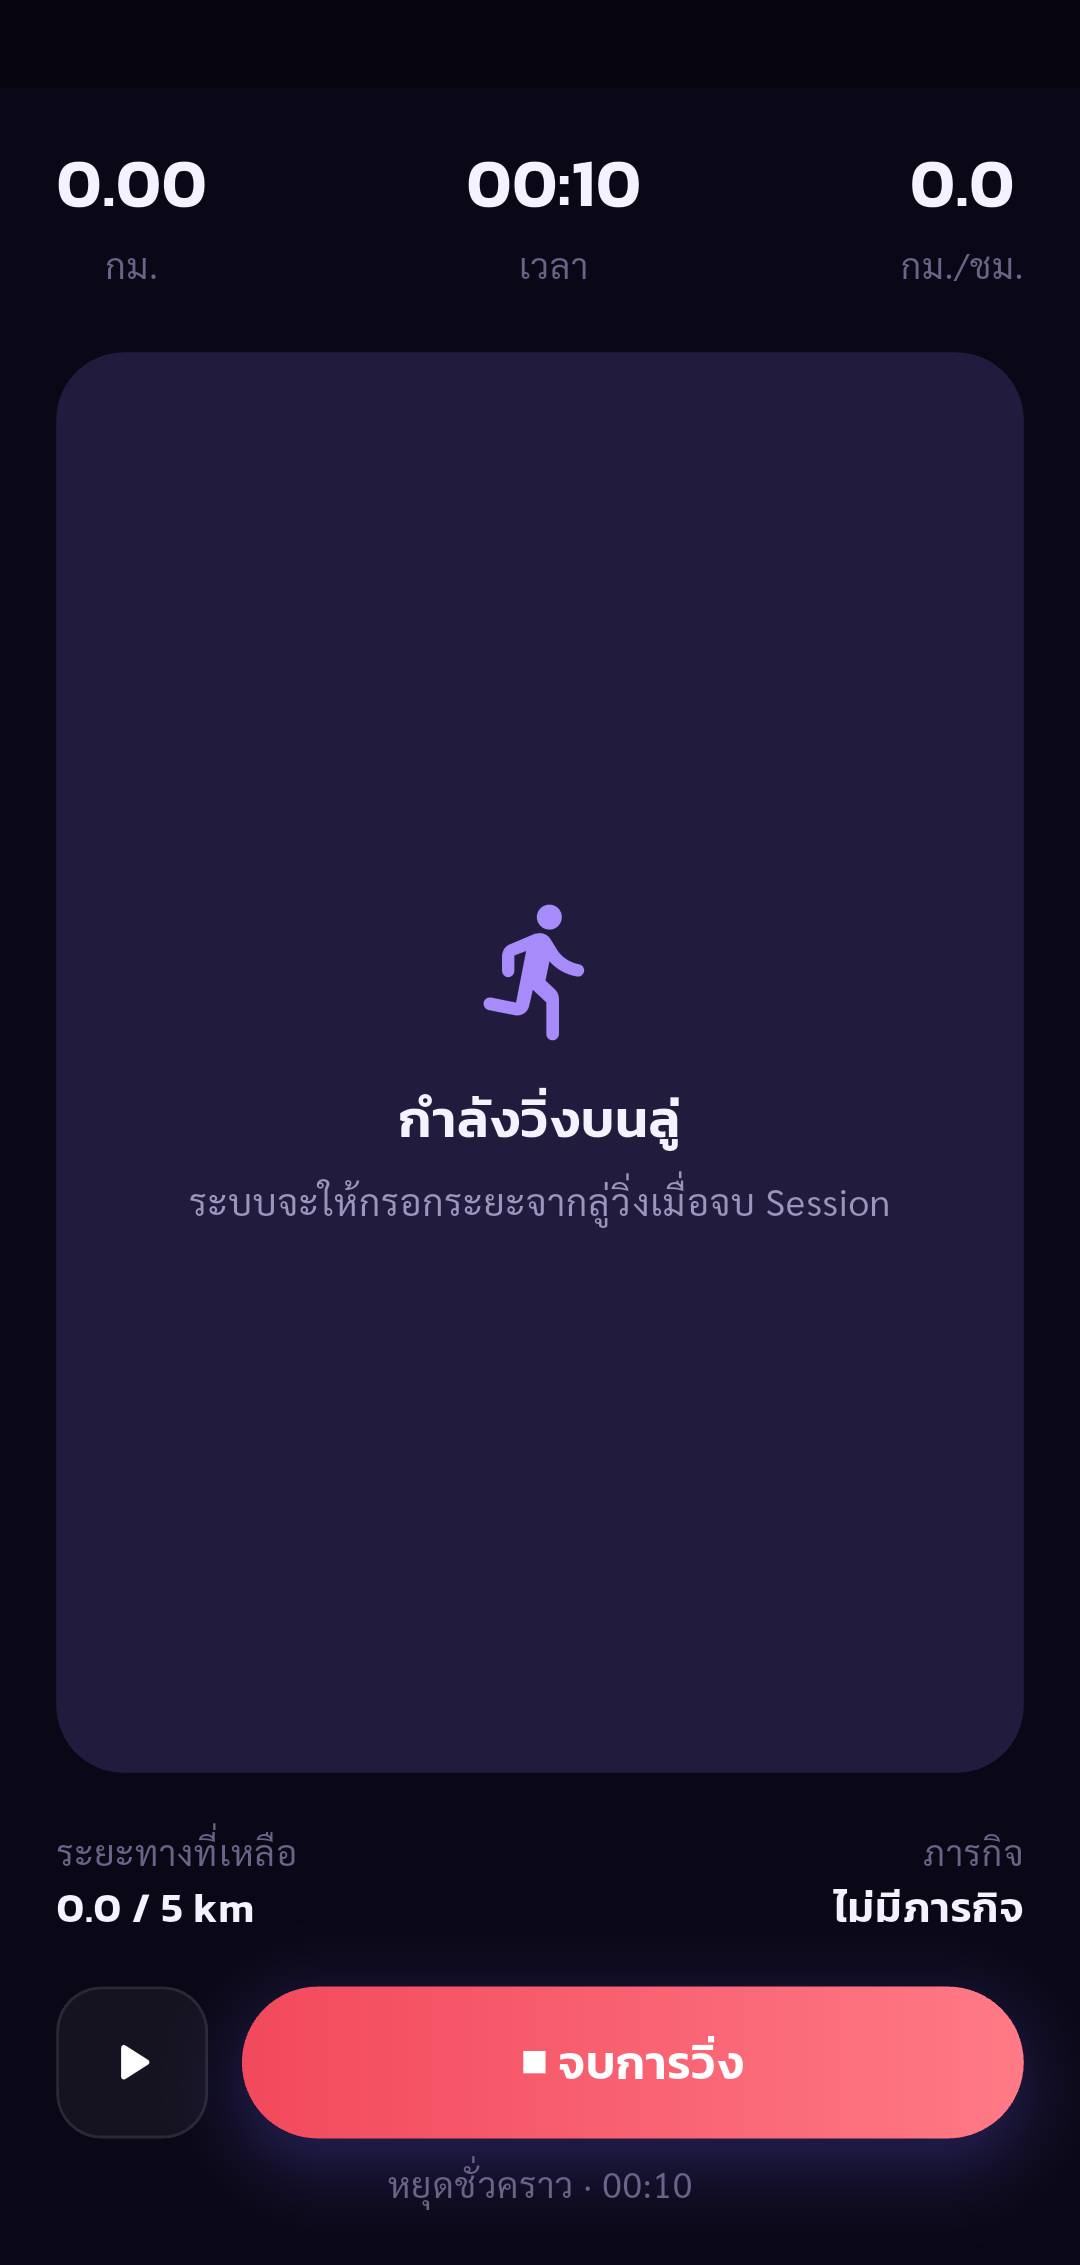
\includegraphics[width=\linewidth,height=0.43\textheight,keepaspectratio]{images/frontend_tests/ft-03-02-run-paused.png}
\caption{พักระหว่างวิ่งในลู่}\end{subfigure}
\hfill
\begin{subfigure}[t]{0.31\textwidth}\centering
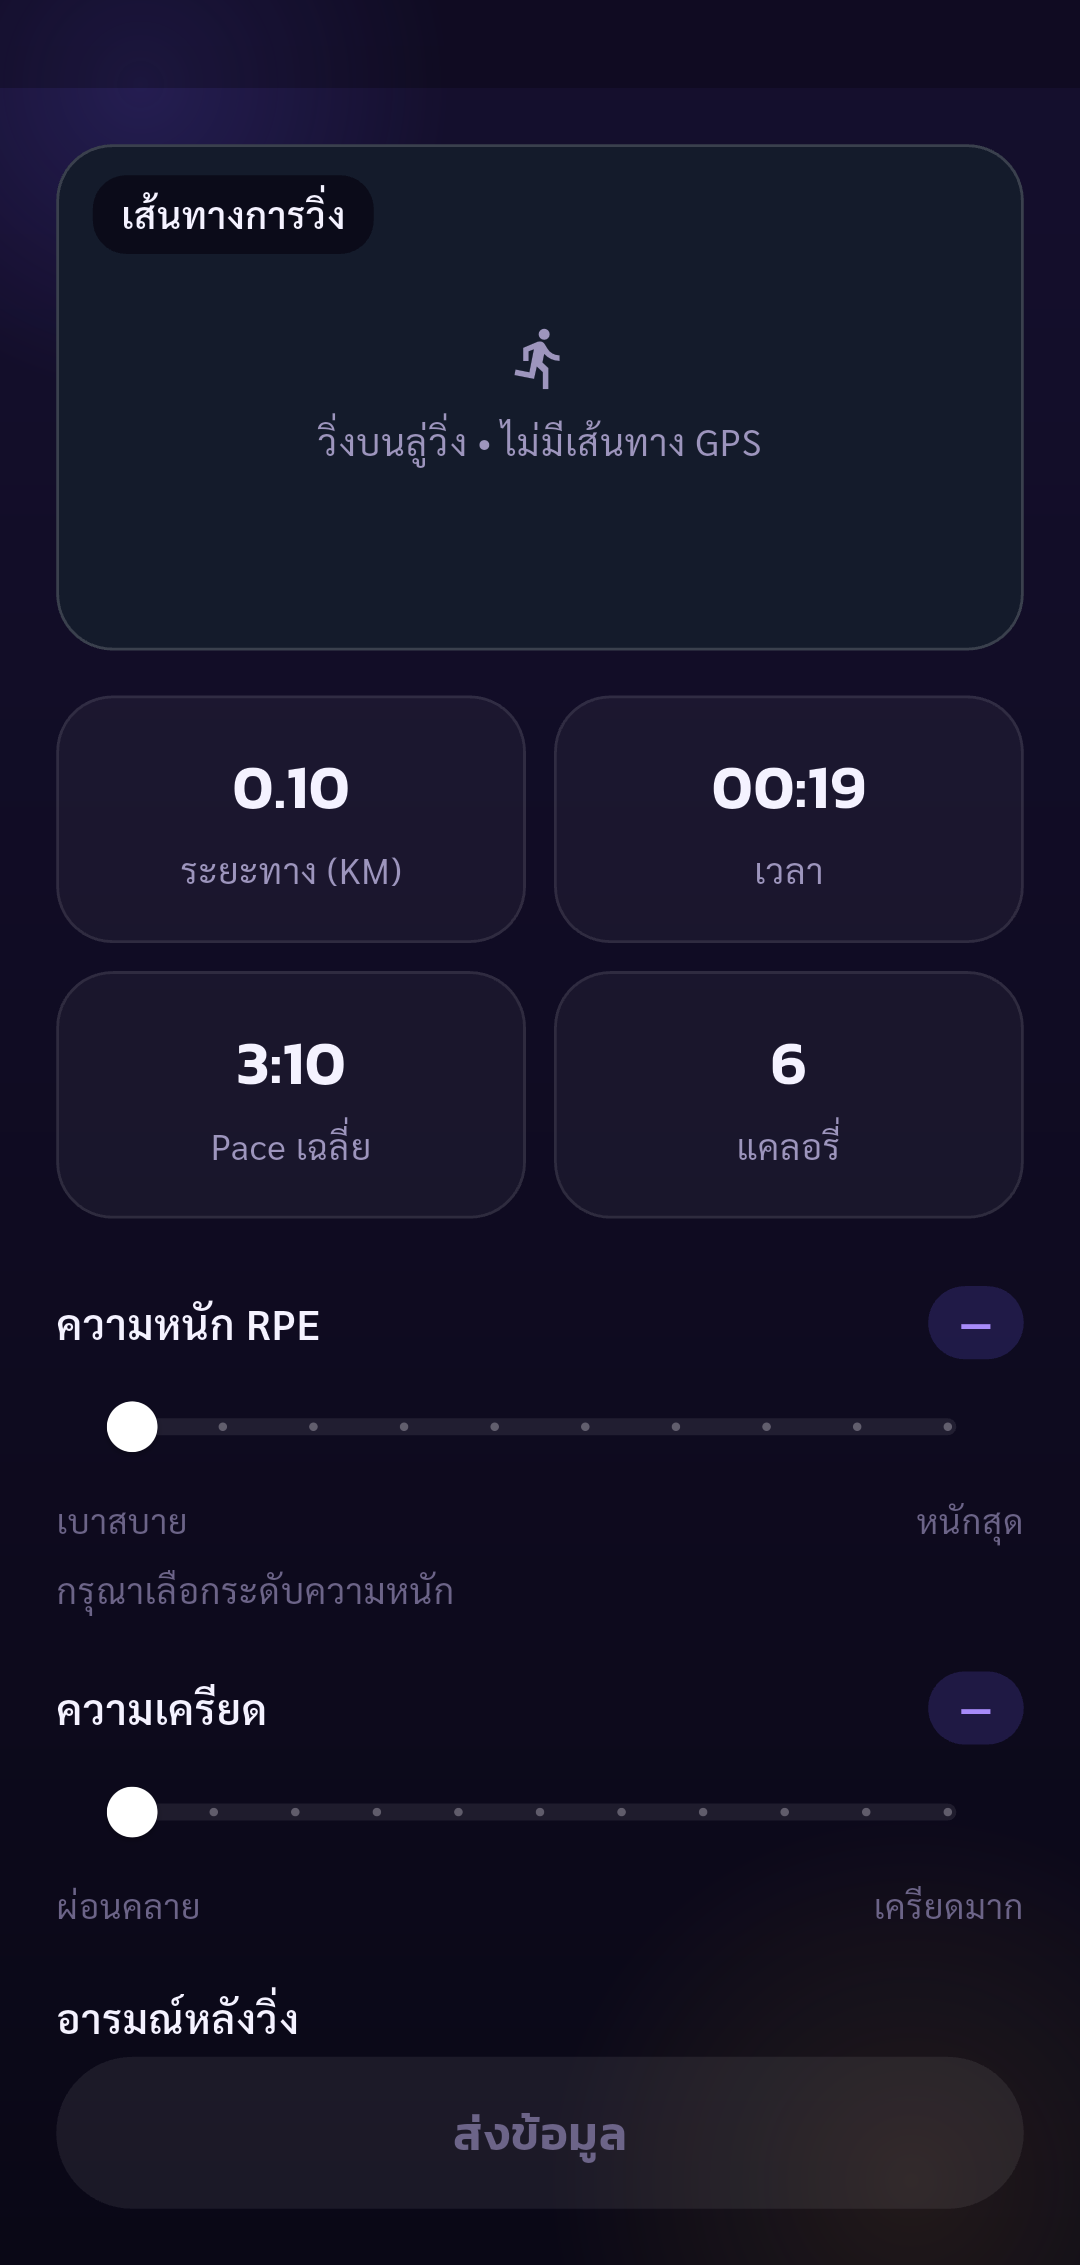
\includegraphics[width=\linewidth,height=0.43\textheight,keepaspectratio]{images/frontend_tests/ft-03-03-run-summary.png}
\caption{สรุปการวิ่งในลู่}\end{subfigure}
\caption{ภาพหลักฐาน FT-03 ชุดที่ 1}\label{fig:flutter-ft-03-1}
\end{figure}

\begin{figure}[H]
\centering
\begin{subfigure}[t]{0.31\textwidth}\centering
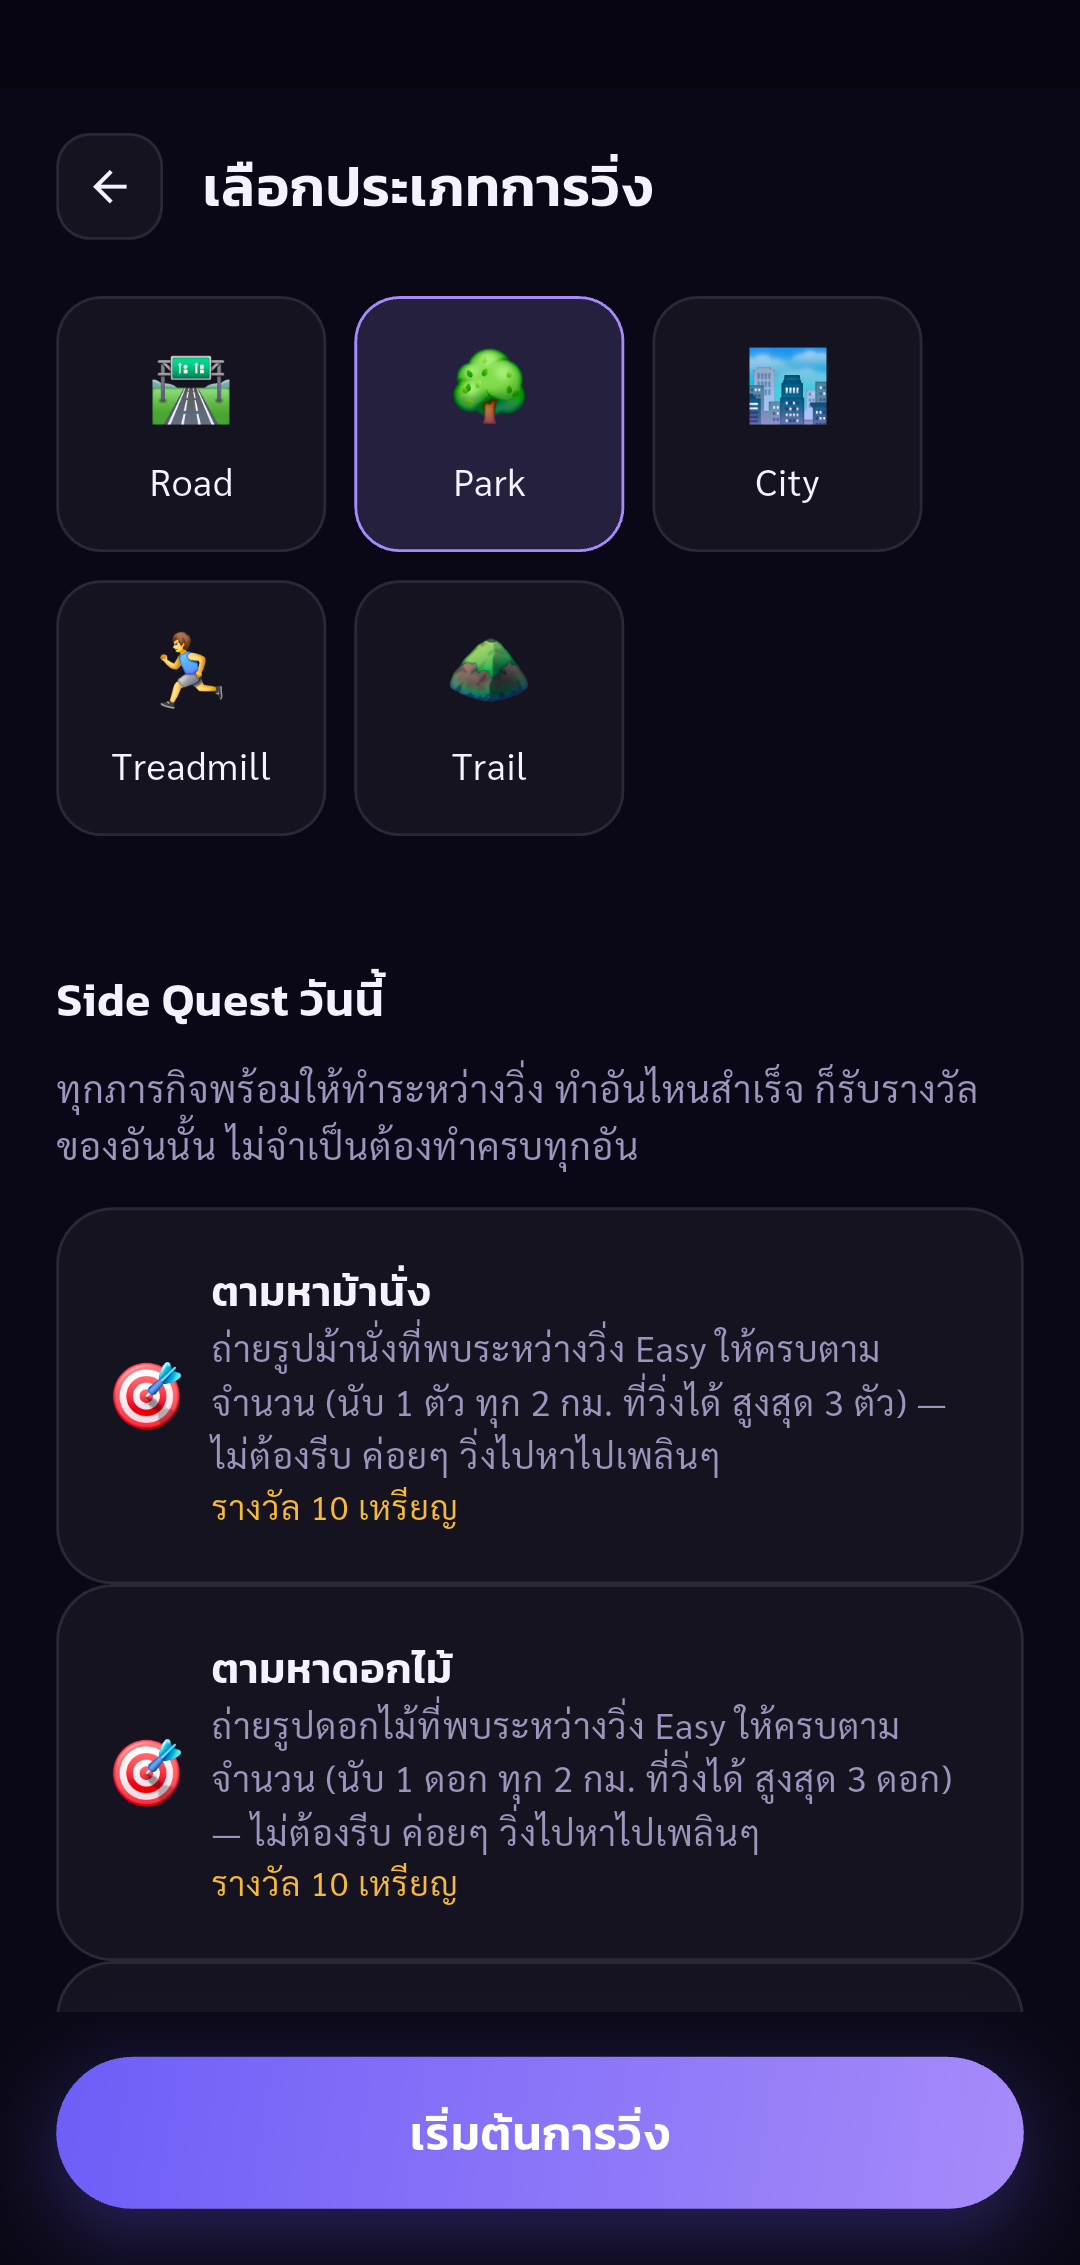
\includegraphics[width=\linewidth,height=0.43\textheight,keepaspectratio]{images/frontend_tests/ft-03-04-run-environment.png}
\caption{เลือกวิ่ง Park}\end{subfigure}
\hfill
\begin{subfigure}[t]{0.31\textwidth}\centering
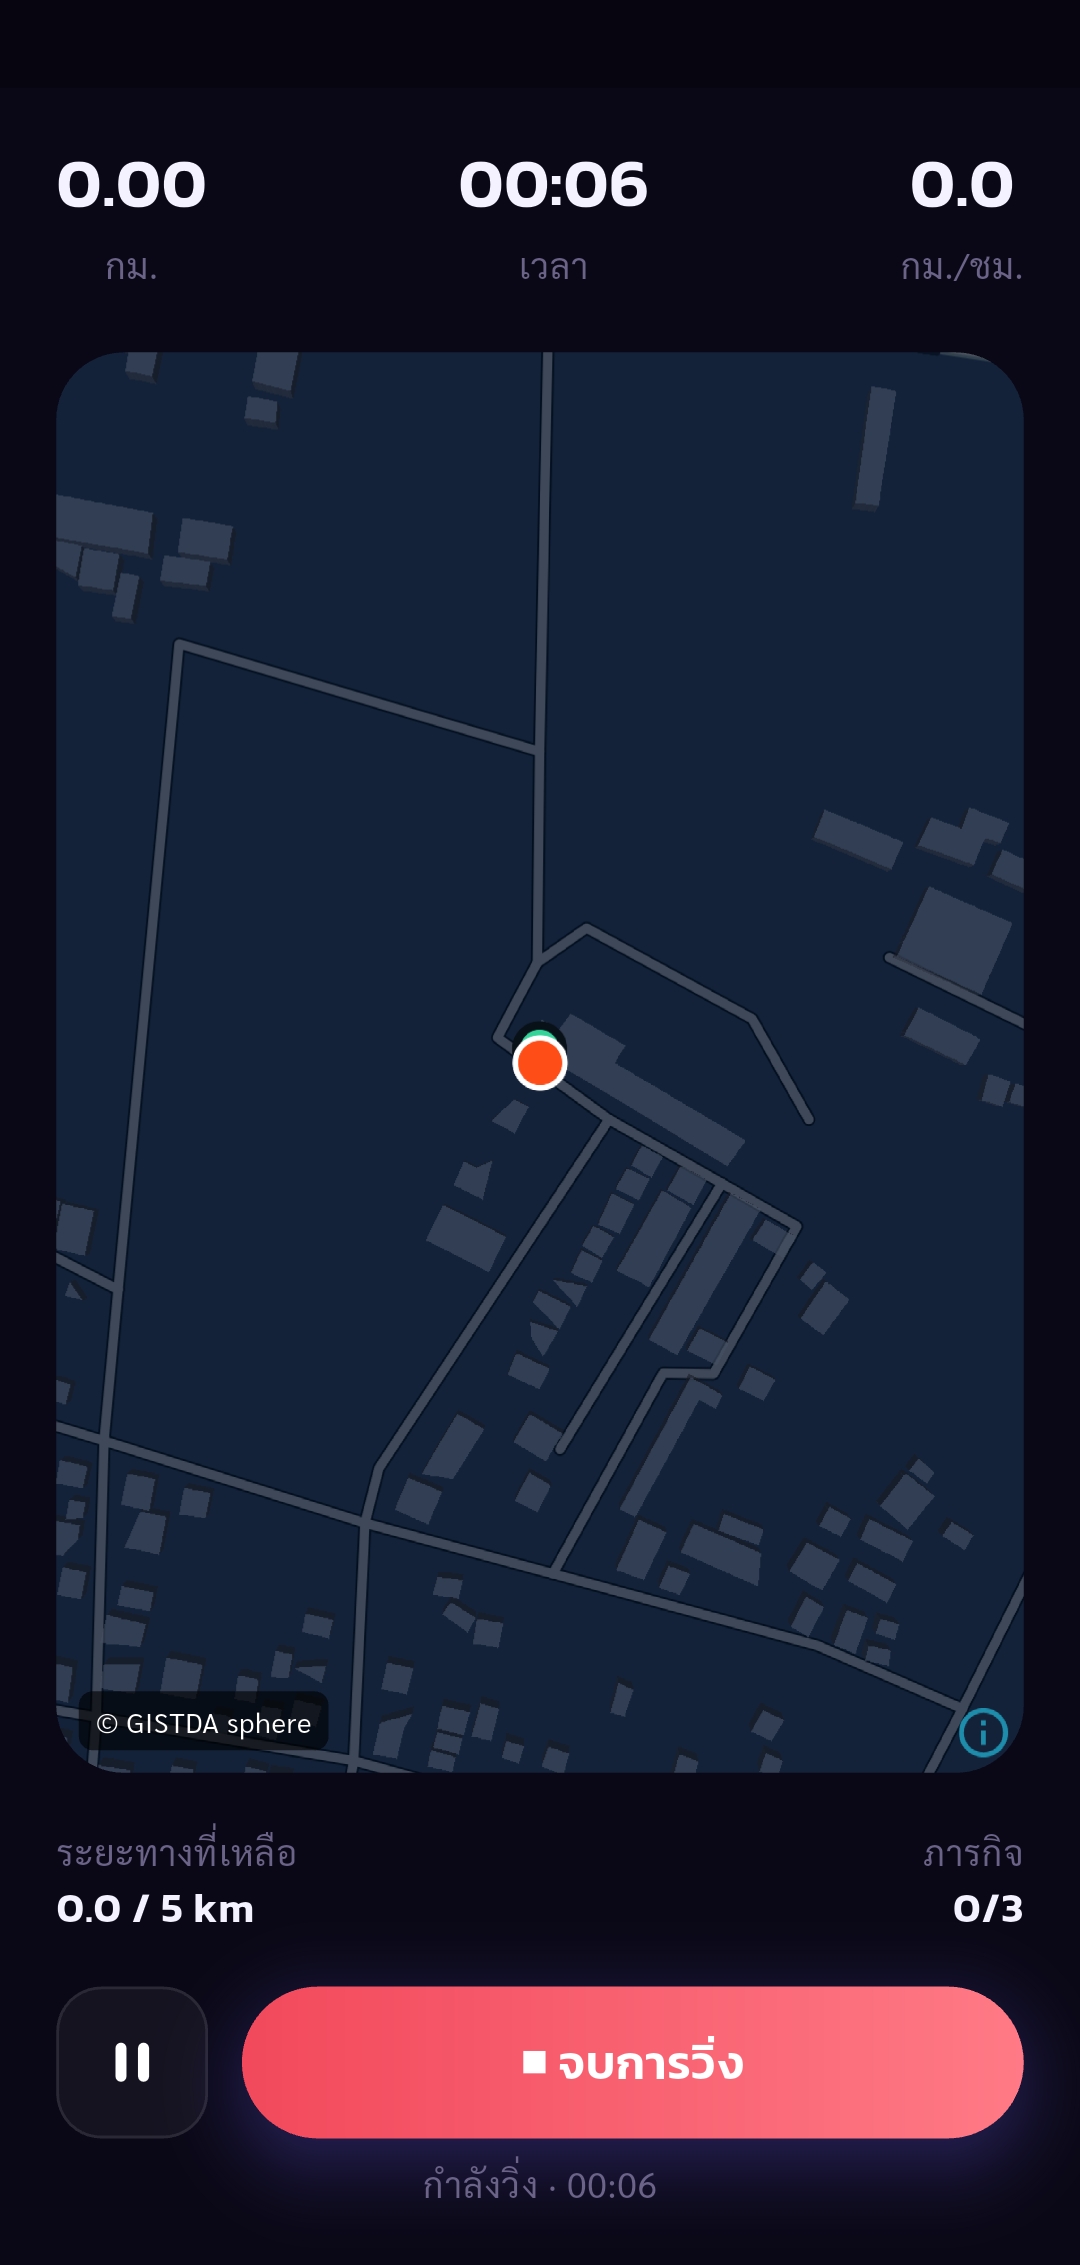
\includegraphics[width=\linewidth,height=0.43\textheight,keepaspectratio]{images/frontend_tests/ft-03-05-park-gps-ready.png}
\caption{ตำแหน่ง GPS พร้อม}\end{subfigure}
\hfill
\begin{subfigure}[t]{0.31\textwidth}\centering
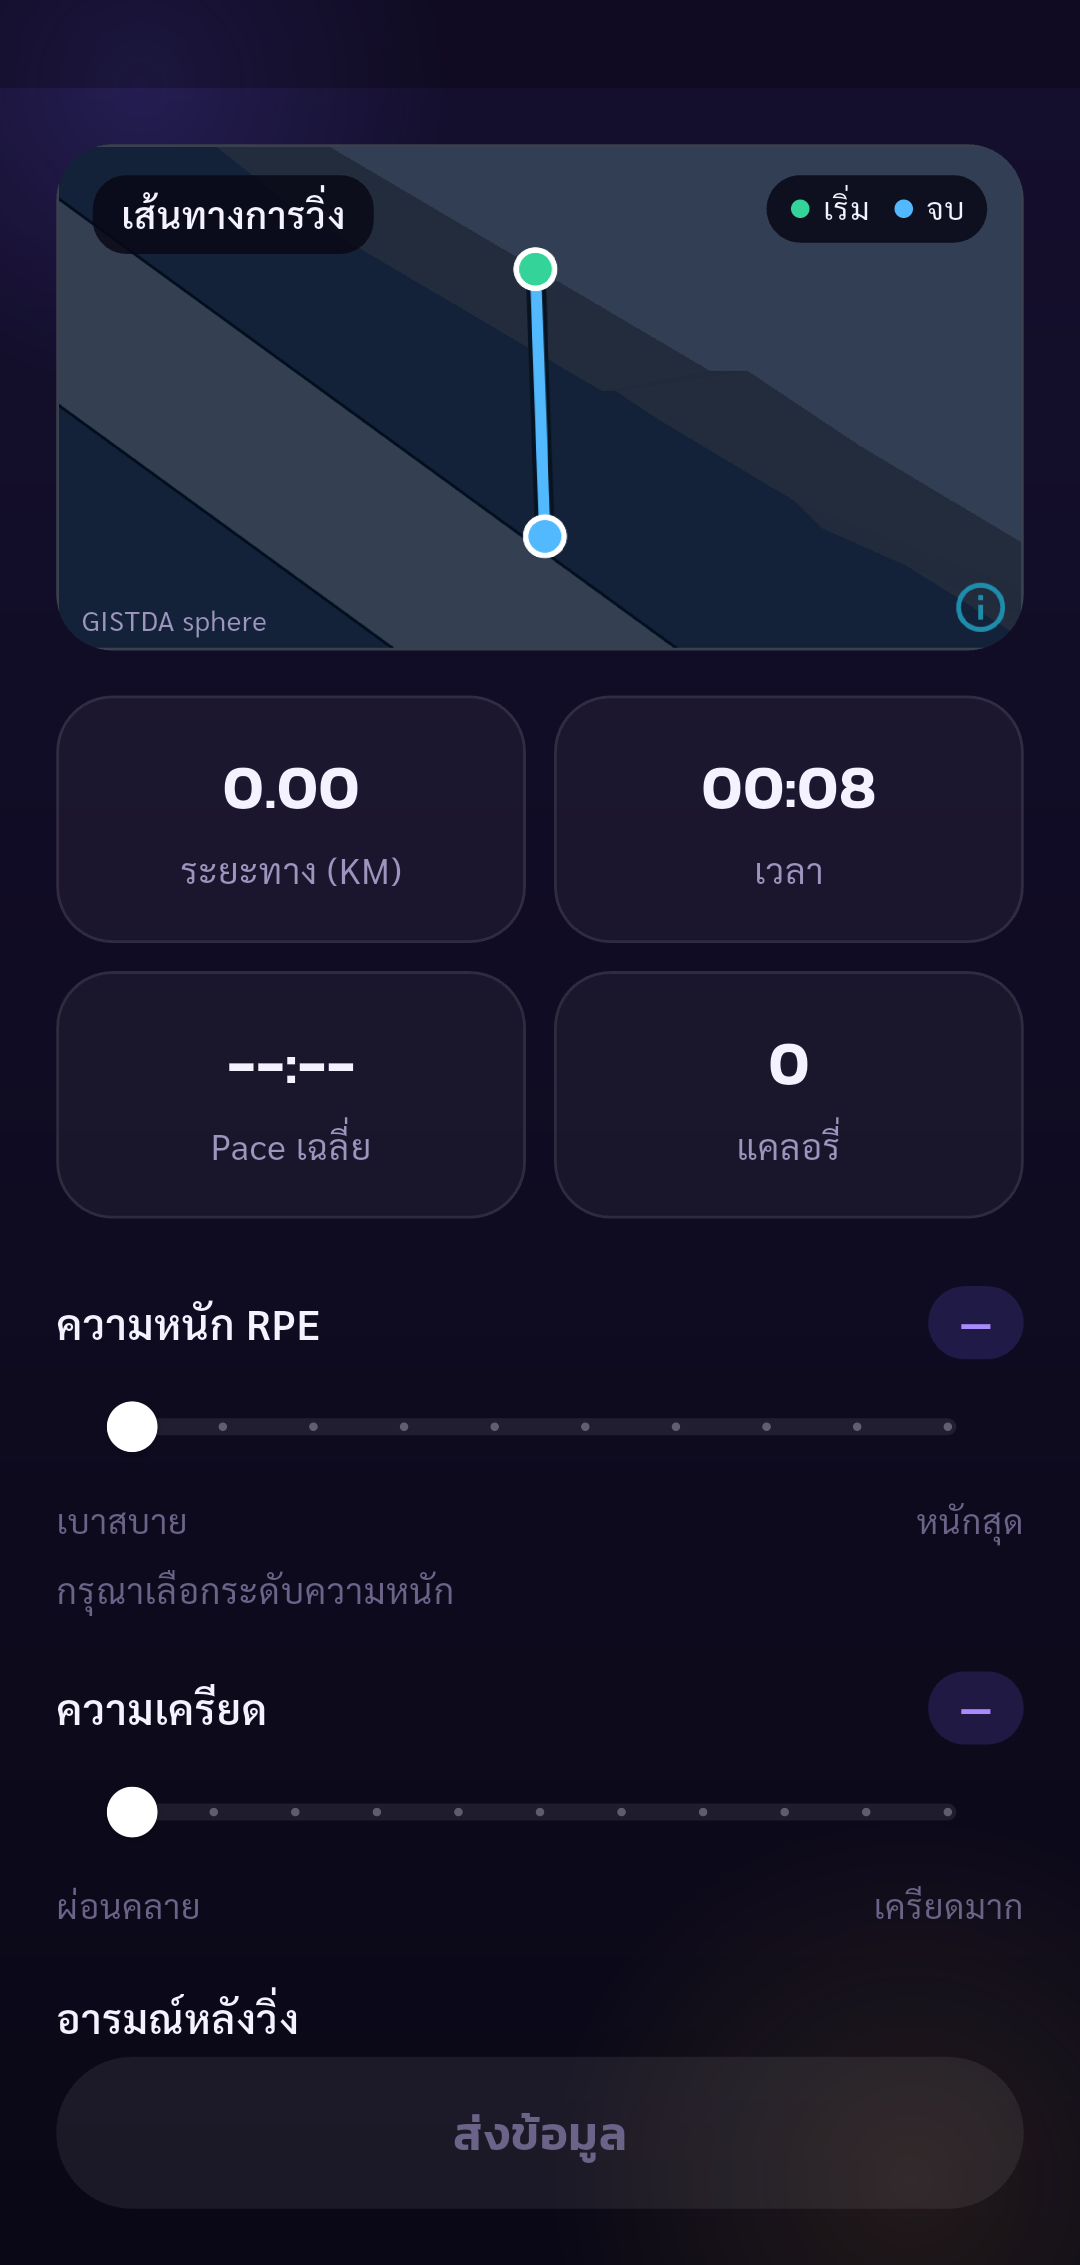
\includegraphics[width=\linewidth,height=0.43\textheight,keepaspectratio]{images/frontend_tests/ft-03-06-run-summary.png}
\caption{สรุปการวิ่ง Park}\end{subfigure}
\caption{ภาพหลักฐาน FT-03 ชุดที่ 2}\label{fig:flutter-ft-03-2}
\end{figure}

\begin{figure}[H]
\centering
\begin{subfigure}[t]{0.31\textwidth}\centering

\includegraphics[width=\linewidth,height=0.43\textheight,keepaspectratio]{images/frontend_tests/ft-03-07-run-reward.png}
\caption{รางวัลหลังจบ Park}\end{subfigure}
\hfill
\begin{subfigure}[t]{0.31\textwidth}\centering
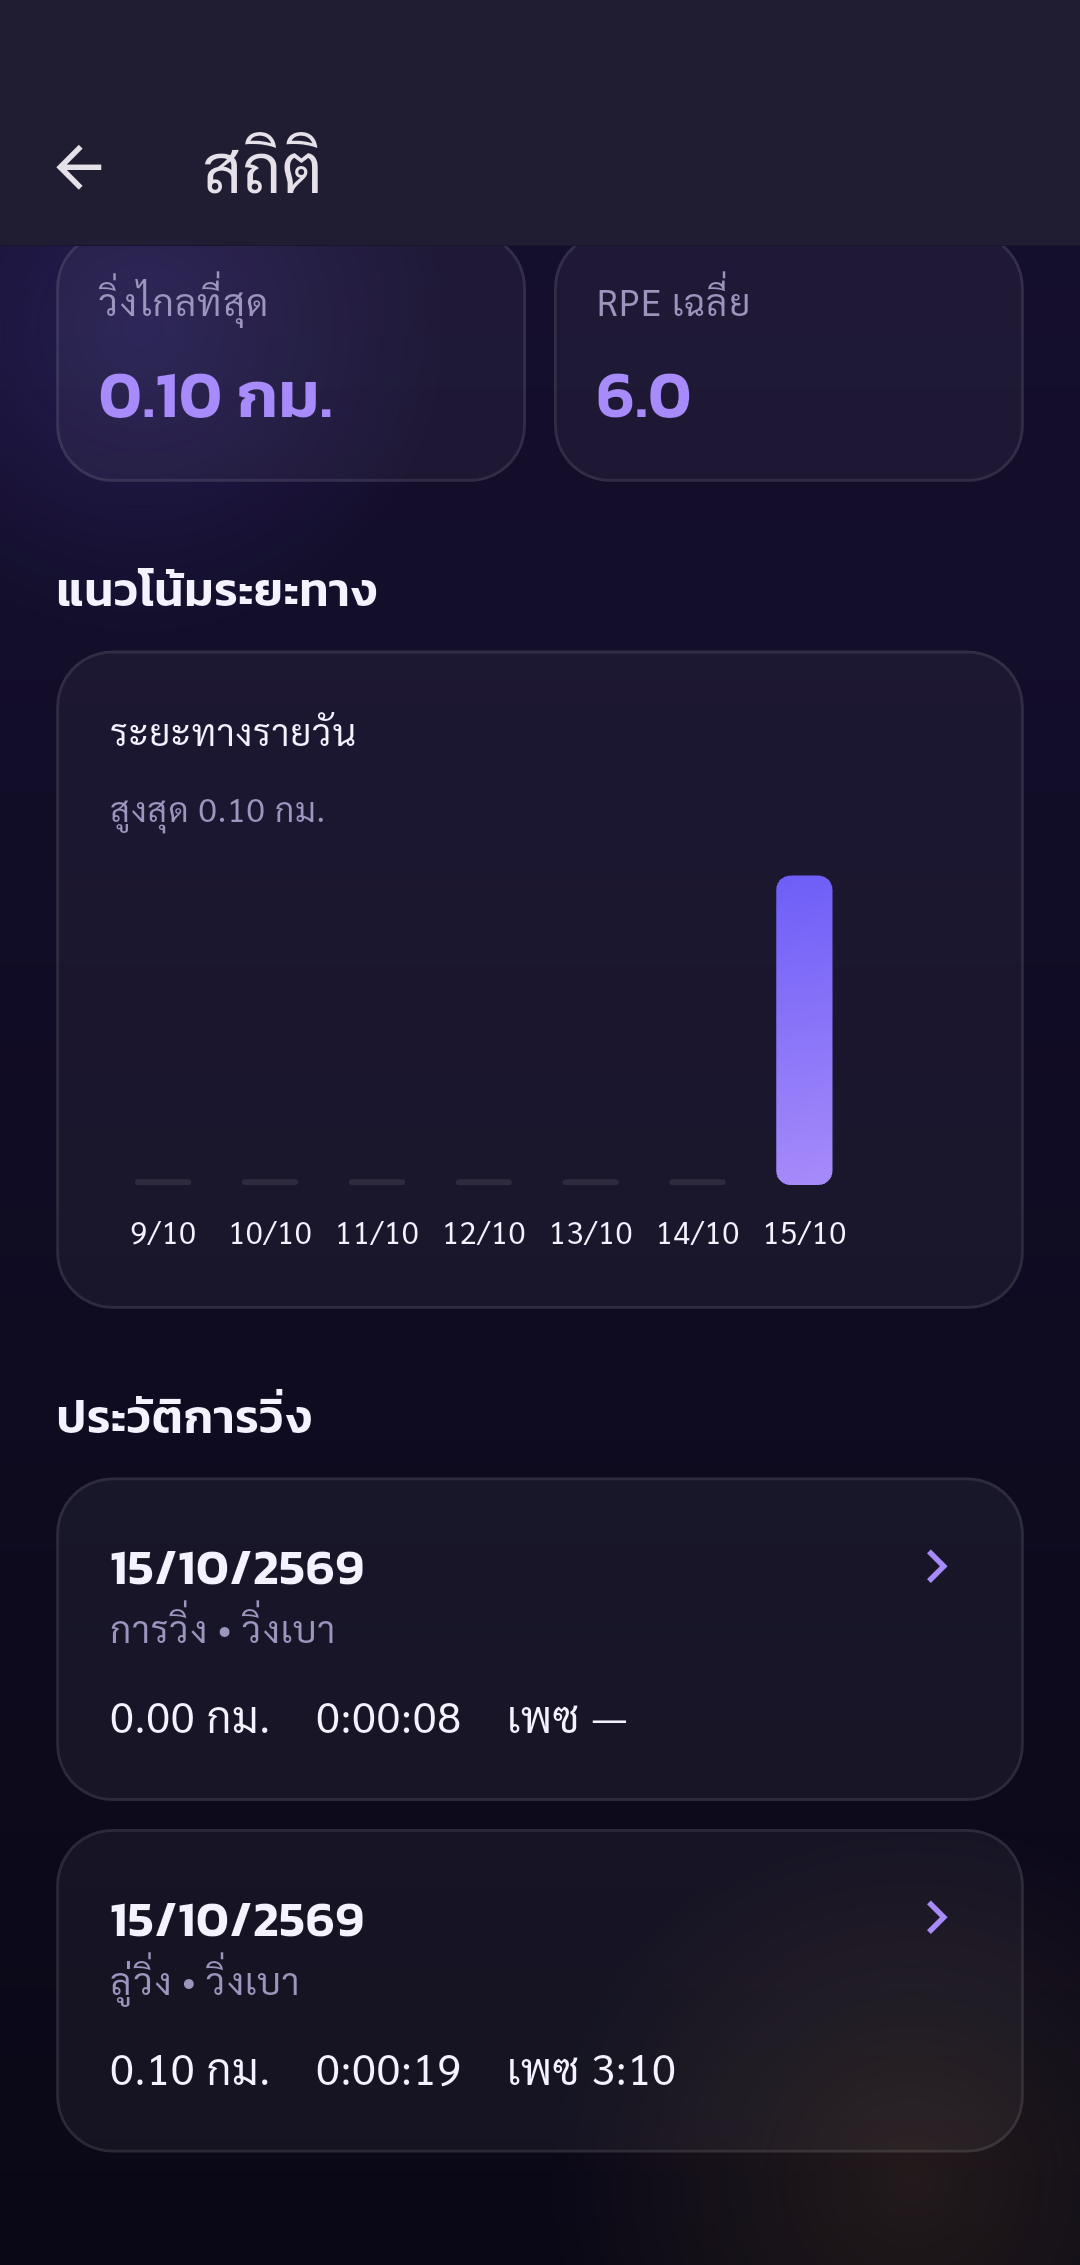
\includegraphics[width=\linewidth,height=0.43\textheight,keepaspectratio]{images/frontend_tests/ft-03-08-run-stats.png}
\caption{สถิติและประวัติ}\end{subfigure}
\hfill
\begin{subfigure}[t]{0.31\textwidth}\centering
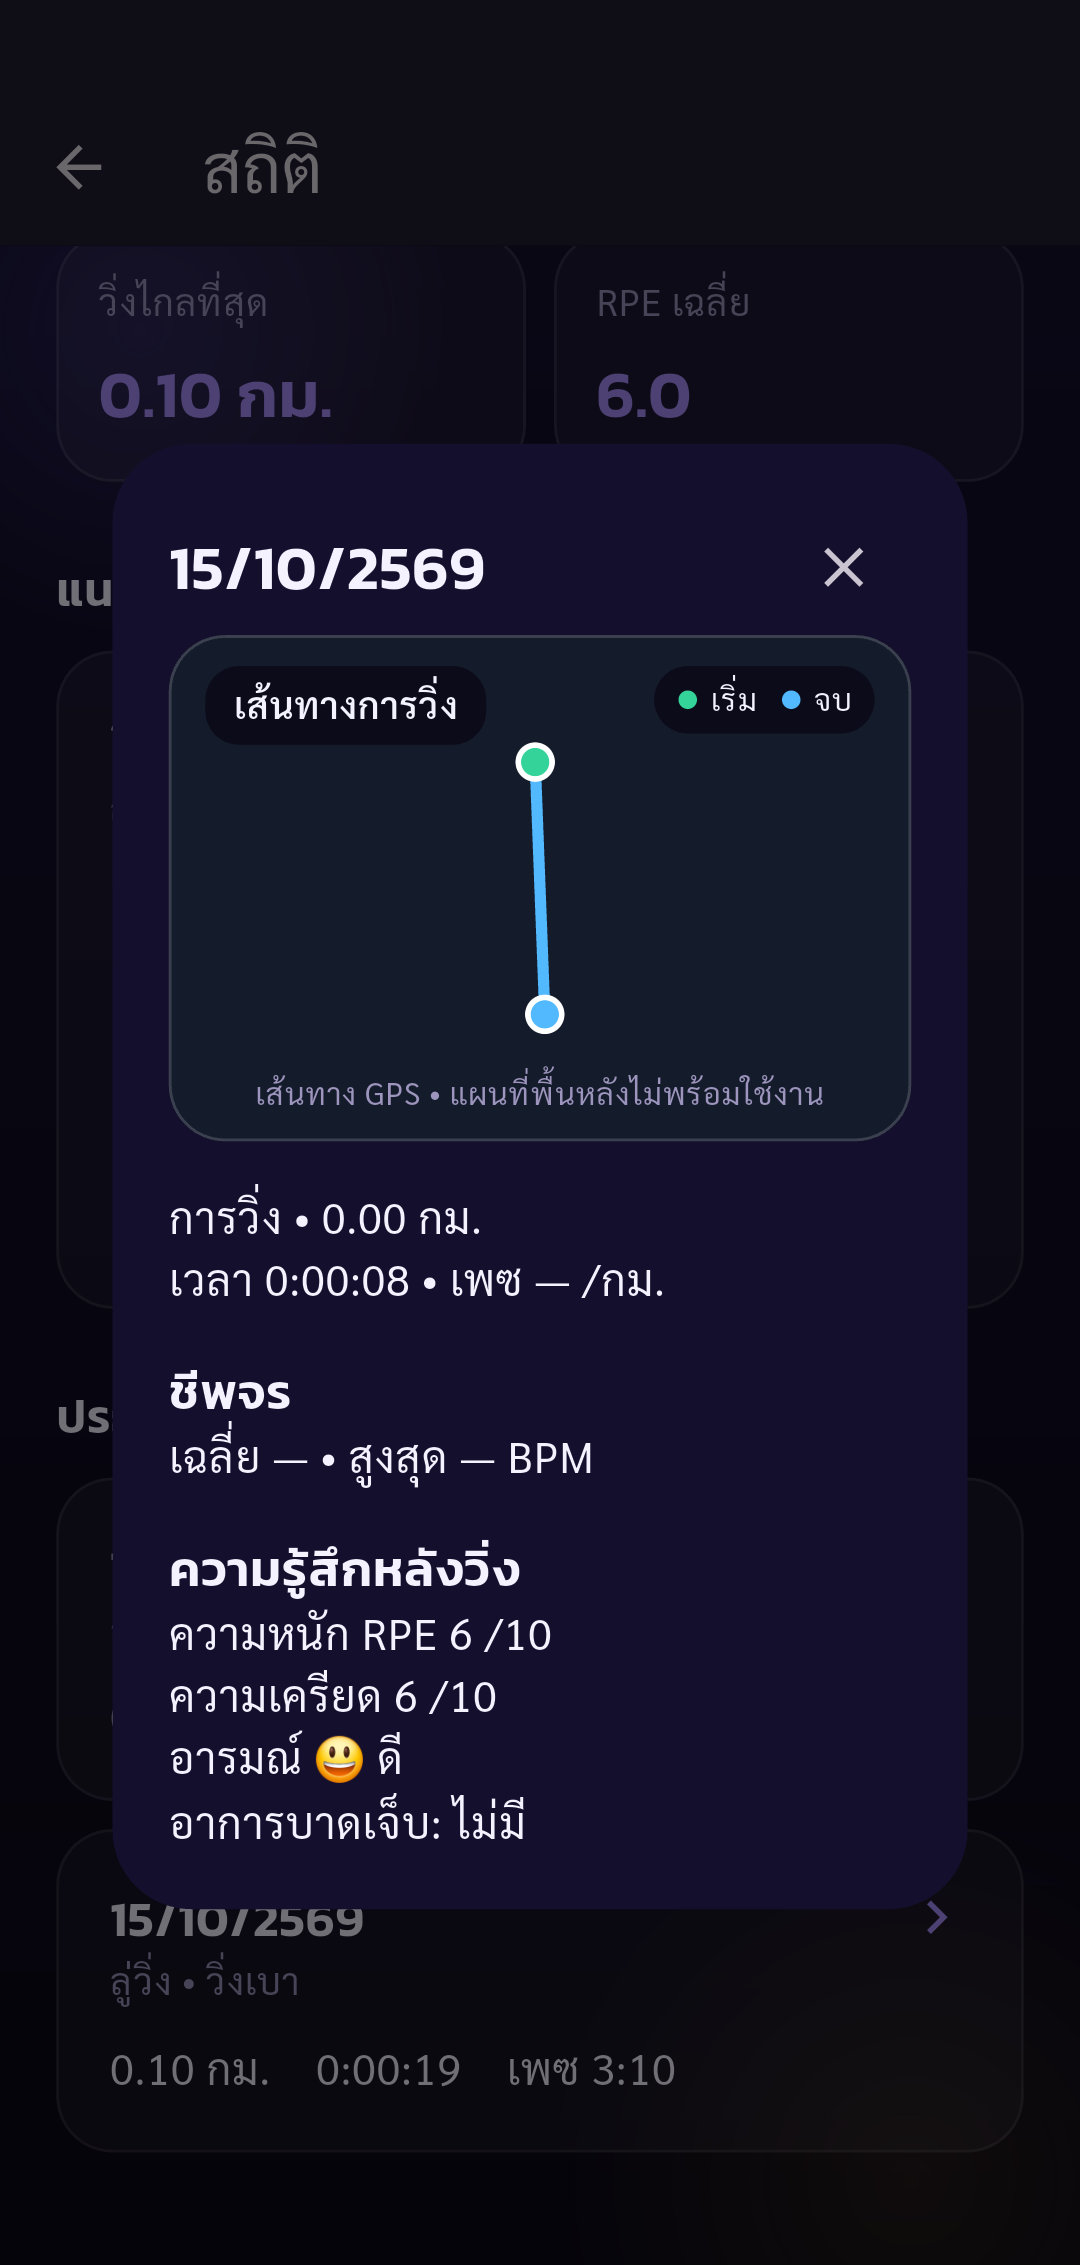
\includegraphics[width=\linewidth,height=0.43\textheight,keepaspectratio]{images/frontend_tests/ft-03-09-run-history-detail.png}
\caption{รายละเอียดประวัติ Park}\end{subfigure}
\caption{ภาพหลักฐาน FT-03 ชุดที่ 3}\label{fig:flutter-ft-03-3}
\end{figure}

\subsubsection{FT-06 ข้อมูลโปรไฟล์ ชื่อ และ UID}

ผลครอบคลุมการปฏิเสธชื่อว่าง การบันทึกชื่อใหม่ การแสดงชื่อบนหน้าหลัก และการคืนชื่อเดิมหลังตรวจสอบ โดย UID ของบัญชีทดสอบไม่เปลี่ยน

\begingroup
\small
\renewcommand{\arraystretch}{1.15}
\begin{longtable}{|>{\raggedright\arraybackslash}p{0.07\textwidth}|>{\raggedright\arraybackslash}p{0.57\textwidth}|>{\raggedright\arraybackslash}p{0.08\textwidth}|>{\raggedright\arraybackslash}p{0.16\textwidth}|}
\caption{ผลการทดสอบ FT-06}\label{tab:flutter-ft-06}\\ \hline
\textbf{ลำดับ} & \textbf{จุดตรวจและผลที่ได้รับจริง} & \textbf{ผล} & \textbf{หลักฐาน} \\ \hline
\endfirsthead
\multicolumn{4}{c}{ผลการทดสอบ FT-06 (ต่อ)} \\ \hline
\textbf{ลำดับ} & \textbf{จุดตรวจและผลที่ได้รับจริง} & \textbf{ผล} & \textbf{หลักฐาน} \\ \hline
\endhead
\endfoot
\endlastfoot
1 & ปฏิเสธชื่อที่มีเฉพาะช่องว่าง และชื่อที่บันทึกไว้ไม่เปลี่ยน & ผ่าน & ภาพที่~\ref{fig:flutter-ft-06-1} (a) \\ \hline
2 & แก้ชื่อแล้วข้อมูลคงอยู่ทั้งใน API จริงและหน้าจอ โดย UID ไม่เปลี่ยน (ตรวจบางส่วนของ SFT-04-002) & ผ่าน & ภาพที่~\ref{fig:flutter-ft-06-1} (b) \\ \hline
3 & หน้าหลักแสดงชื่อใหม่ที่บันทึก โดยรอโมเดลแสดงผล 3 วินาทีก่อนบันทึกภาพ & ผ่าน & ภาพที่~\ref{fig:flutter-ft-06-1} (c) \\ \hline
4 & คืนชื่อเดิมผ่านหน้าจอและตรวจยืนยันกับเซิร์ฟเวอร์ โดยไม่ออกจากระบบหรือลบบัญชี & ผ่าน & ภาพที่~\ref{fig:flutter-ft-06-2} (a) \\ \hline
\end{longtable}
\endgroup

\begin{figure}[H]
\centering
\begin{subfigure}[t]{0.31\textwidth}\centering
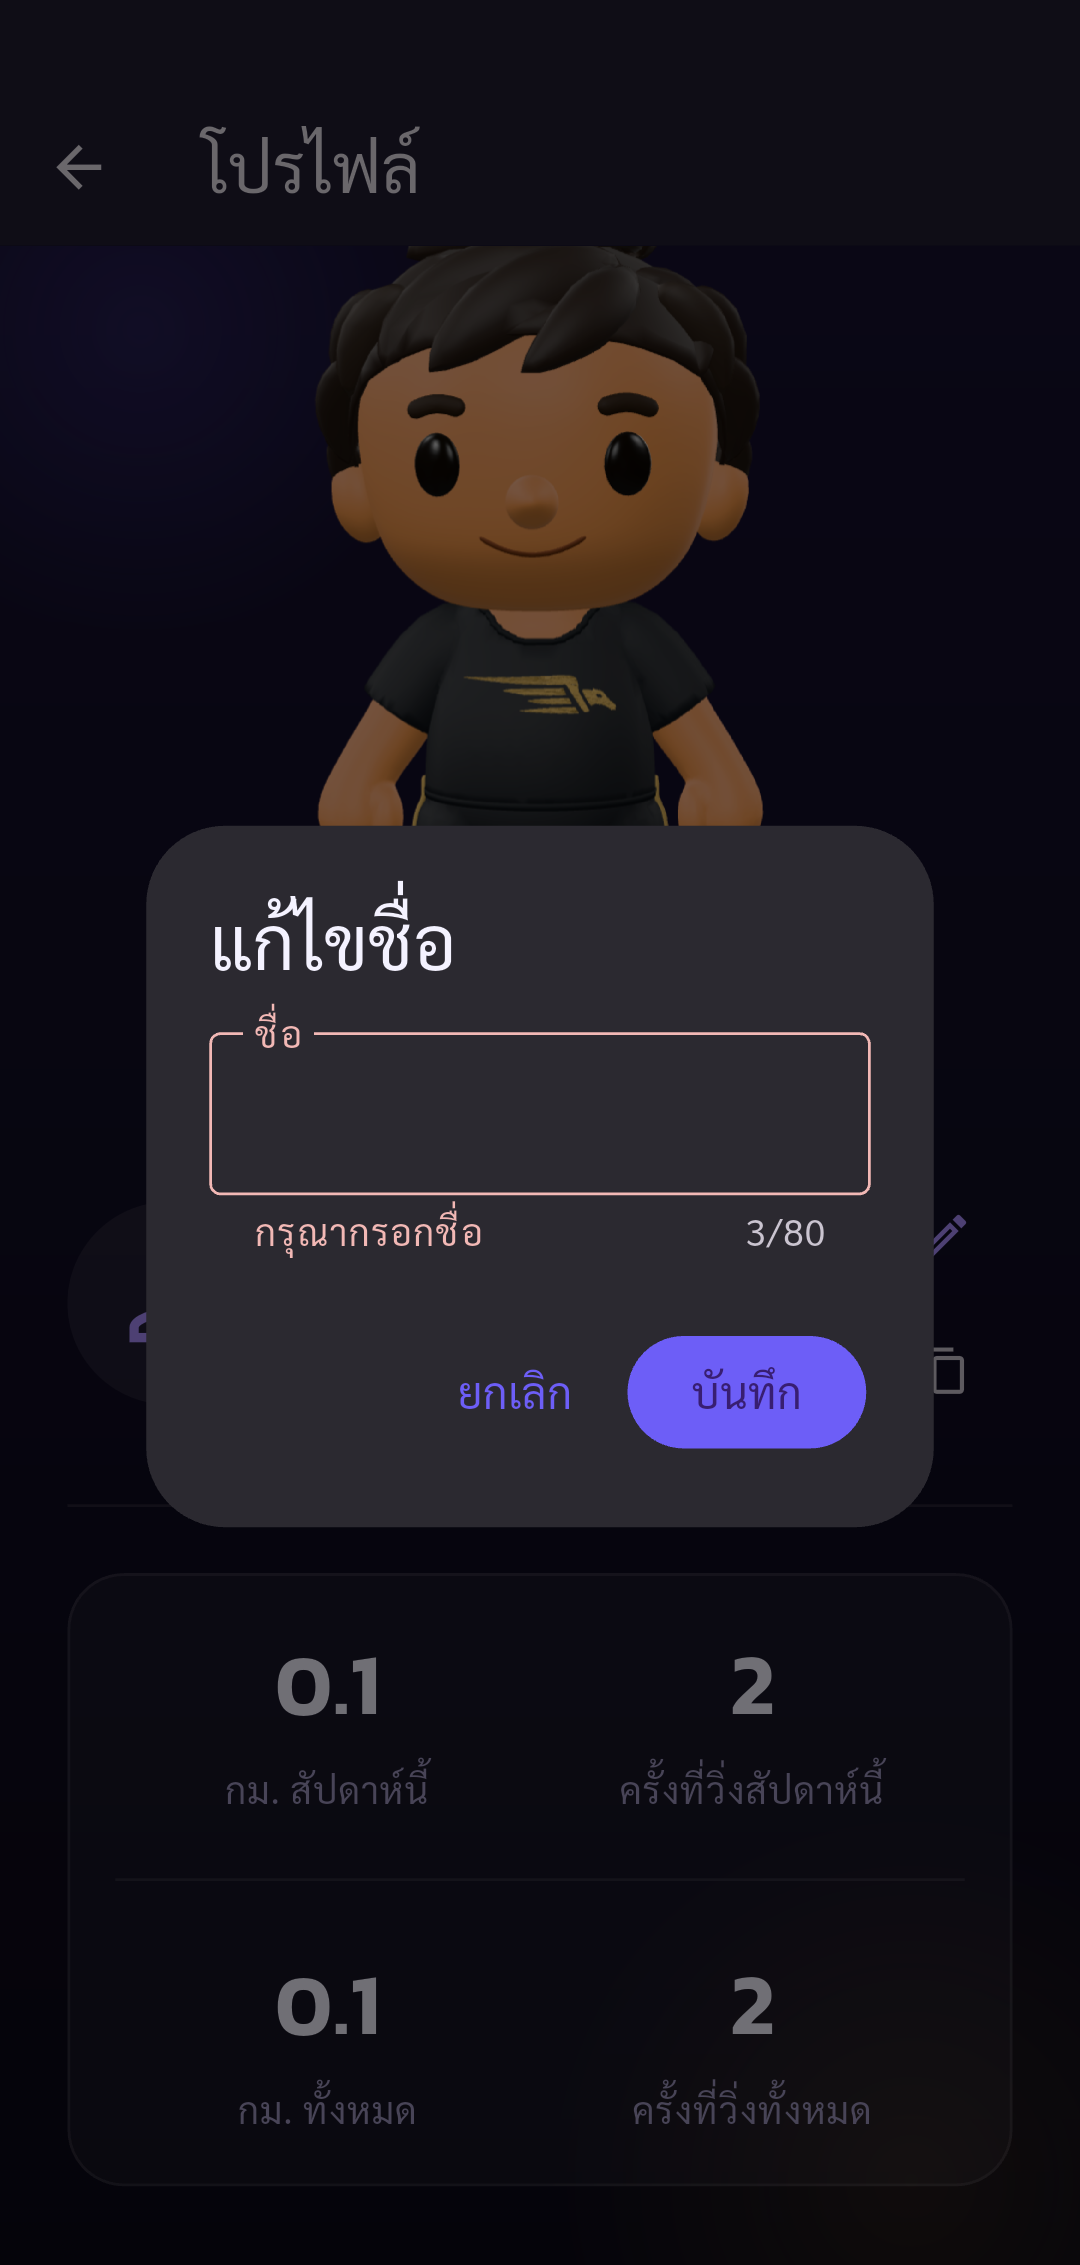
\includegraphics[width=\linewidth,height=0.43\textheight,keepaspectratio]{images/frontend_tests/ft-06-01-profile-empty-rejected.png}
\caption{ปฏิเสธชื่อว่าง}\end{subfigure}
\hfill
\begin{subfigure}[t]{0.31\textwidth}\centering
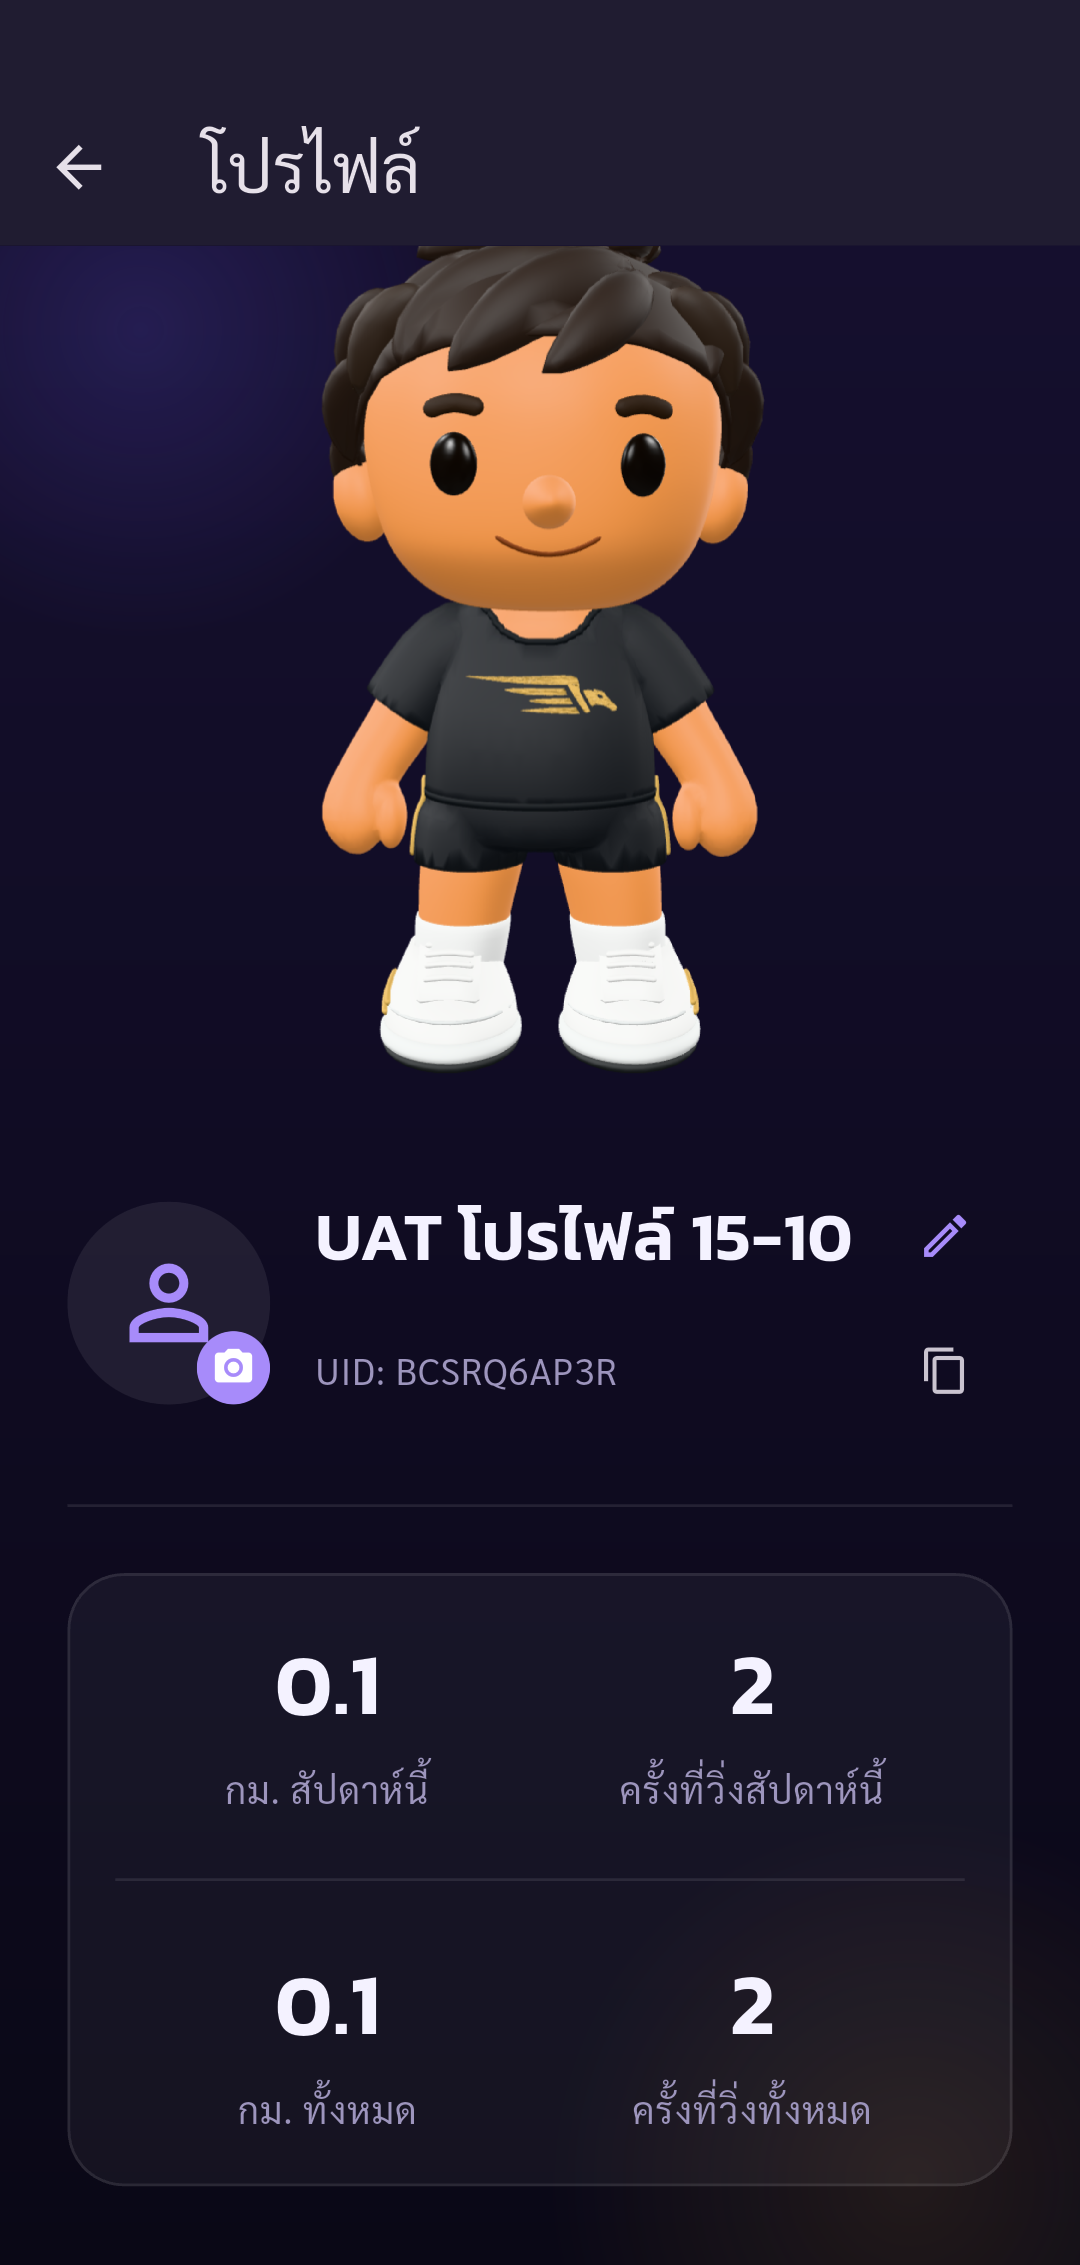
\includegraphics[width=\linewidth,height=0.43\textheight,keepaspectratio]{images/frontend_tests/ft-06-02-profile-name.png}
\caption{บันทึกชื่อใหม่}\end{subfigure}
\hfill
\begin{subfigure}[t]{0.31\textwidth}\centering

\includegraphics[width=\linewidth,height=0.43\textheight,keepaspectratio]{images/frontend_tests/ft-06-03-profile-home-name.png}
\caption{ชื่อใหม่บนหน้าหลัก}\end{subfigure}
\caption{ภาพหลักฐาน FT-06 ชุดที่ 1}\label{fig:flutter-ft-06-1}
\end{figure}

\begin{figure}[H]
\centering
\begin{subfigure}[t]{0.31\textwidth}\centering
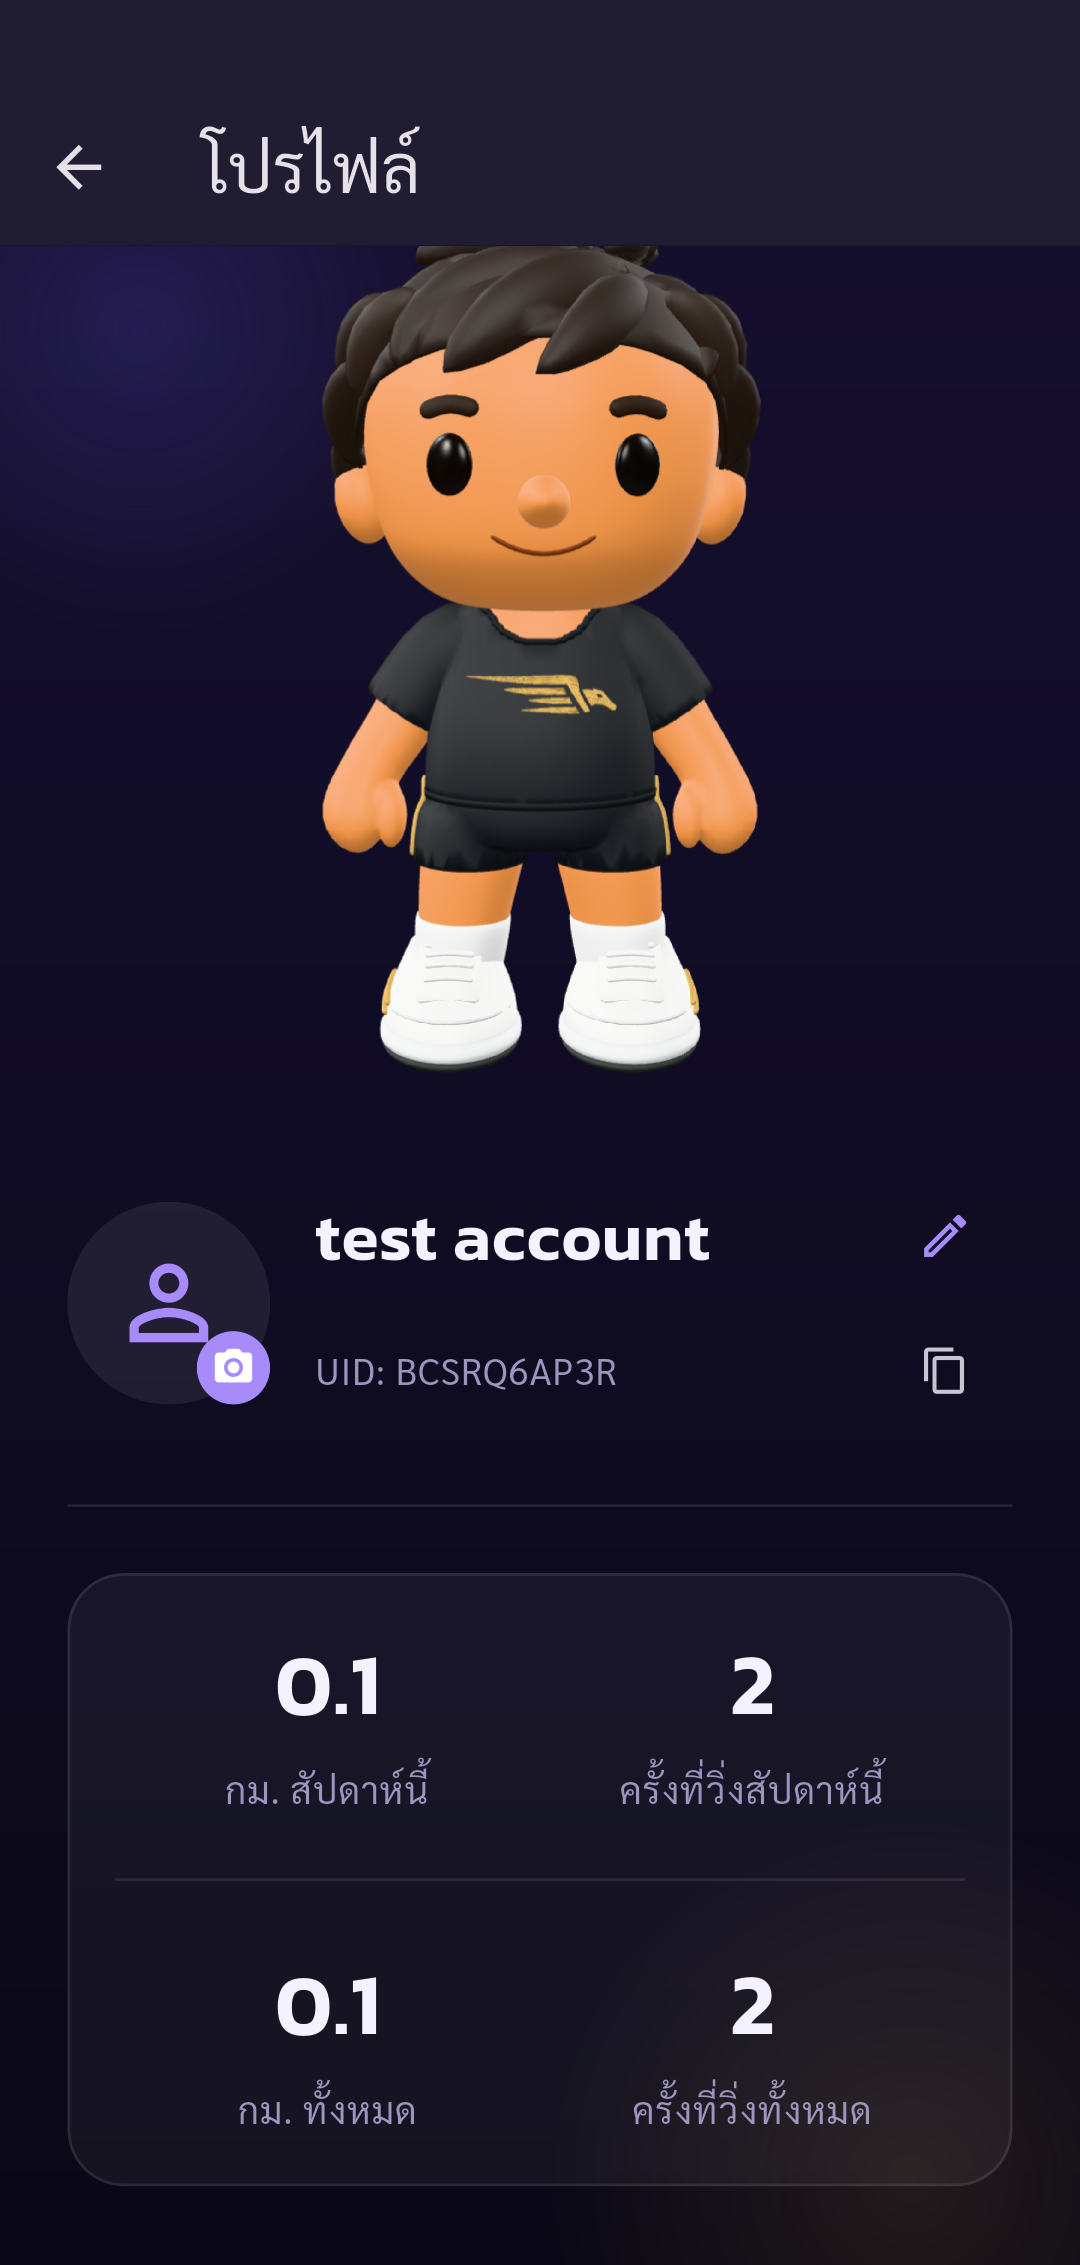
\includegraphics[width=\linewidth,height=0.43\textheight,keepaspectratio]{images/frontend_tests/ft-06-04-profile-original-name-restored.png}
\caption{คืนชื่อเดิม}\end{subfigure}
\caption{ภาพหลักฐาน FT-06 ชุดที่ 2}\label{fig:flutter-ft-06-2}
\end{figure}

\subsubsection{FT-07 เปลี่ยนภาพโปรไฟล์}

รายงานระบุว่าเลือกภาพล่าสุดจากคลังภาพของโทรศัพท์ อัปโหลดจริง ตรวจว่าที่อยู่ภาพเปลี่ยน ภาพแสดงผลได้ และชื่อกับ UID ไม่เปลี่ยน ภาพใหม่ยังถูกใช้งานหลังเปิดโปรไฟล์ซ้ำ

\begingroup
\small
\renewcommand{\arraystretch}{1.15}
\begin{longtable}{|>{\raggedright\arraybackslash}p{0.07\textwidth}|>{\raggedright\arraybackslash}p{0.57\textwidth}|>{\raggedright\arraybackslash}p{0.08\textwidth}|>{\raggedright\arraybackslash}p{0.16\textwidth}|}
\caption{ผลการทดสอบ FT-07}\label{tab:flutter-ft-07}\\ \hline
\textbf{ลำดับ} & \textbf{จุดตรวจและผลที่ได้รับจริง} & \textbf{ผล} & \textbf{หลักฐาน} \\ \hline
\endfirsthead
\multicolumn{4}{c}{ผลการทดสอบ FT-07 (ต่อ)} \\ \hline
\textbf{ลำดับ} & \textbf{จุดตรวจและผลที่ได้รับจริง} & \textbf{ผล} & \textbf{หลักฐาน} \\ \hline
\endhead
\endfoot
\endlastfoot
1 & เปิดโปรไฟล์ก่อนเปลี่ยนภาพ โดยชื่อและ UID ตรงกับบัญชีเดิม & ผ่าน & ภาพที่~\ref{fig:flutter-ft-07-1} (a) \\ \hline
2 & เปิดโปรไฟล์ใหม่แล้วโหลดภาพใหม่เดิมจากเซิร์ฟเวอร์และถอดรหัสภาพเพื่อแสดงบนหน้าจอสำเร็จ & ผ่าน & ภาพที่~\ref{fig:flutter-ft-07-1} (b) \\ \hline
\end{longtable}
\endgroup

\begin{figure}[H]
\centering
\begin{subfigure}[t]{0.31\textwidth}\centering
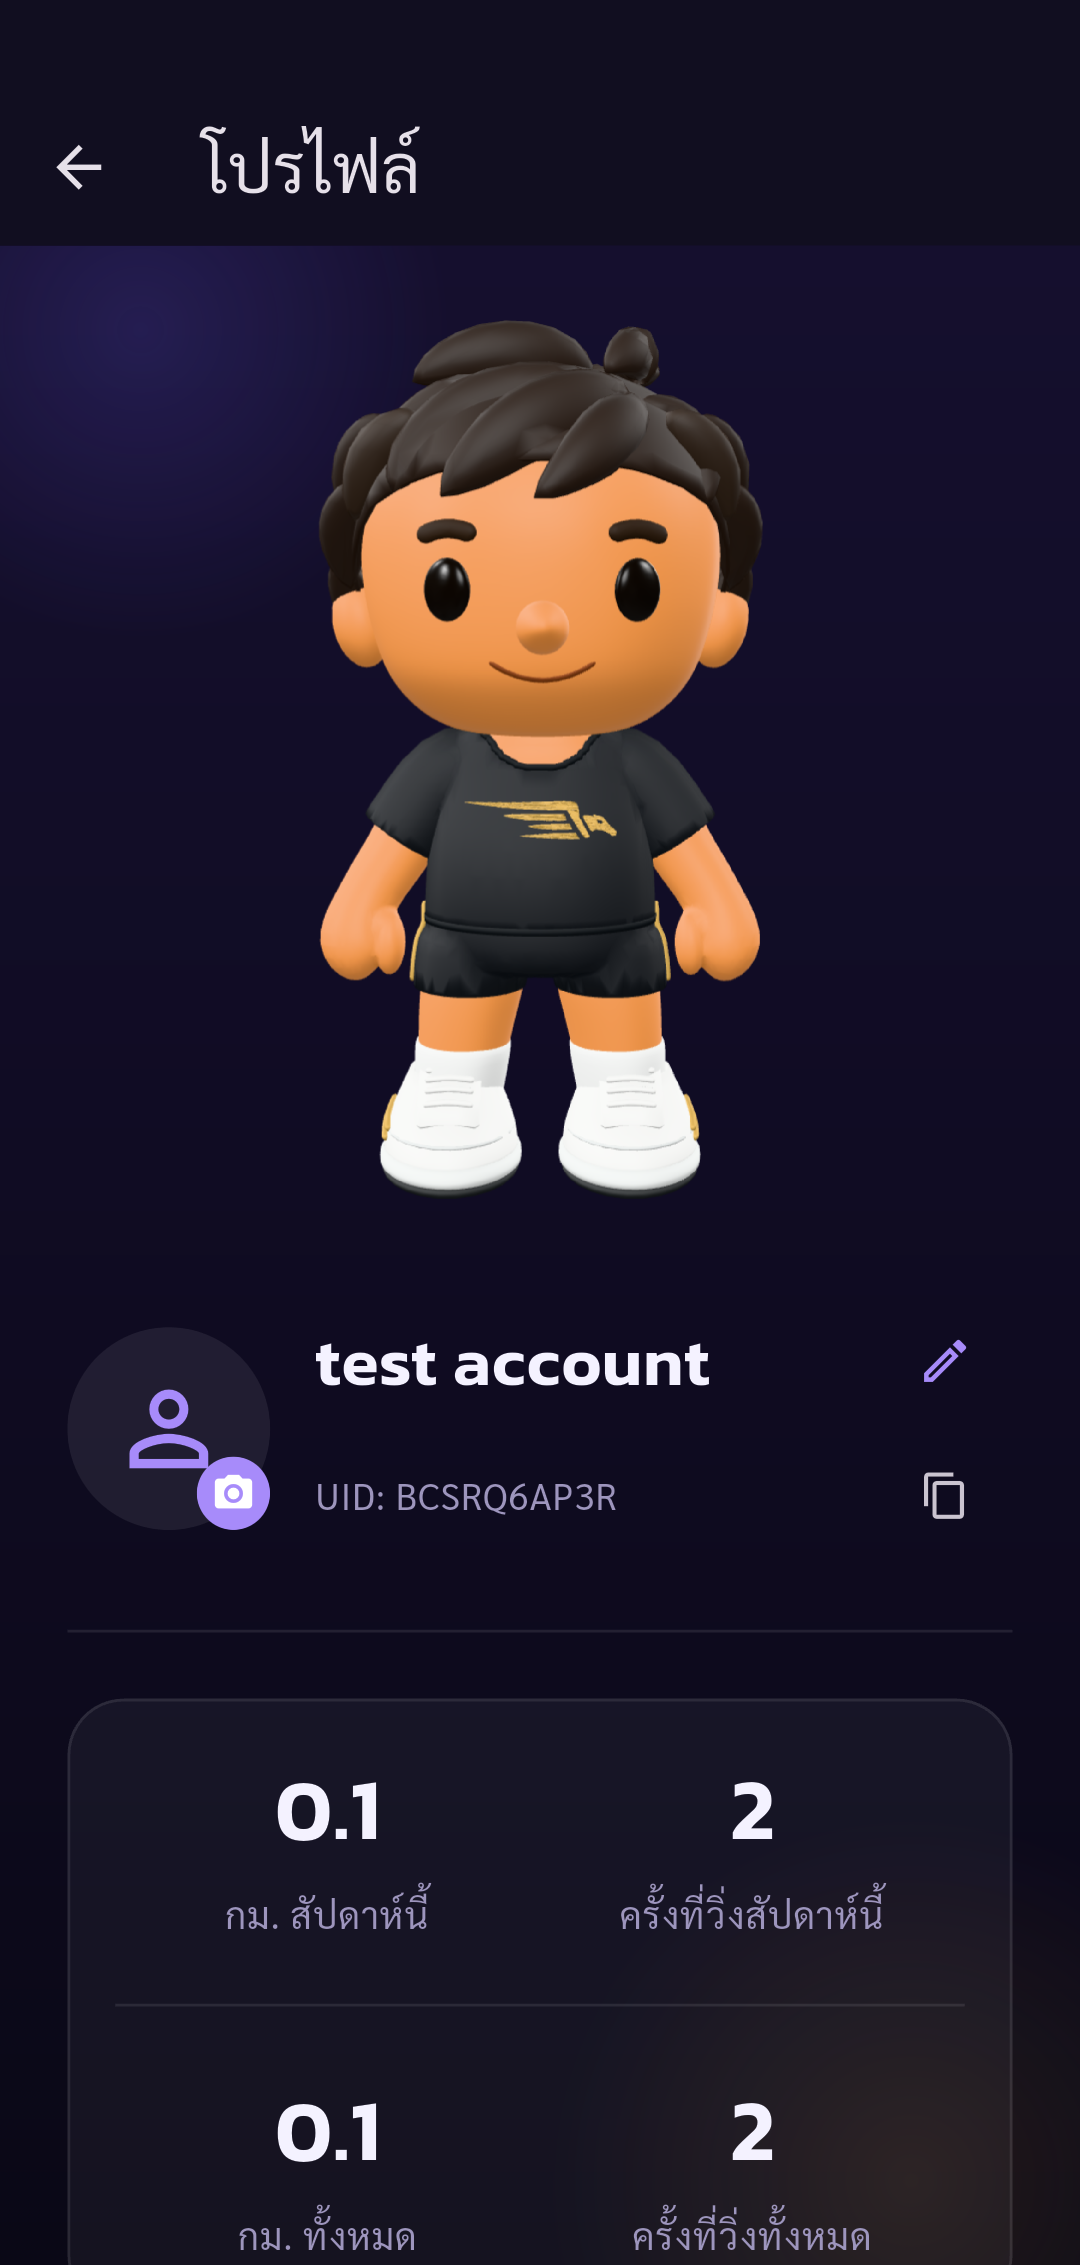
\includegraphics[width=\linewidth,height=0.43\textheight,keepaspectratio]{images/frontend_tests/ft-07-01-photo-before.png}
\caption{ก่อนเปลี่ยนภาพ}\end{subfigure}
\hfill
\begin{subfigure}[t]{0.31\textwidth}\centering
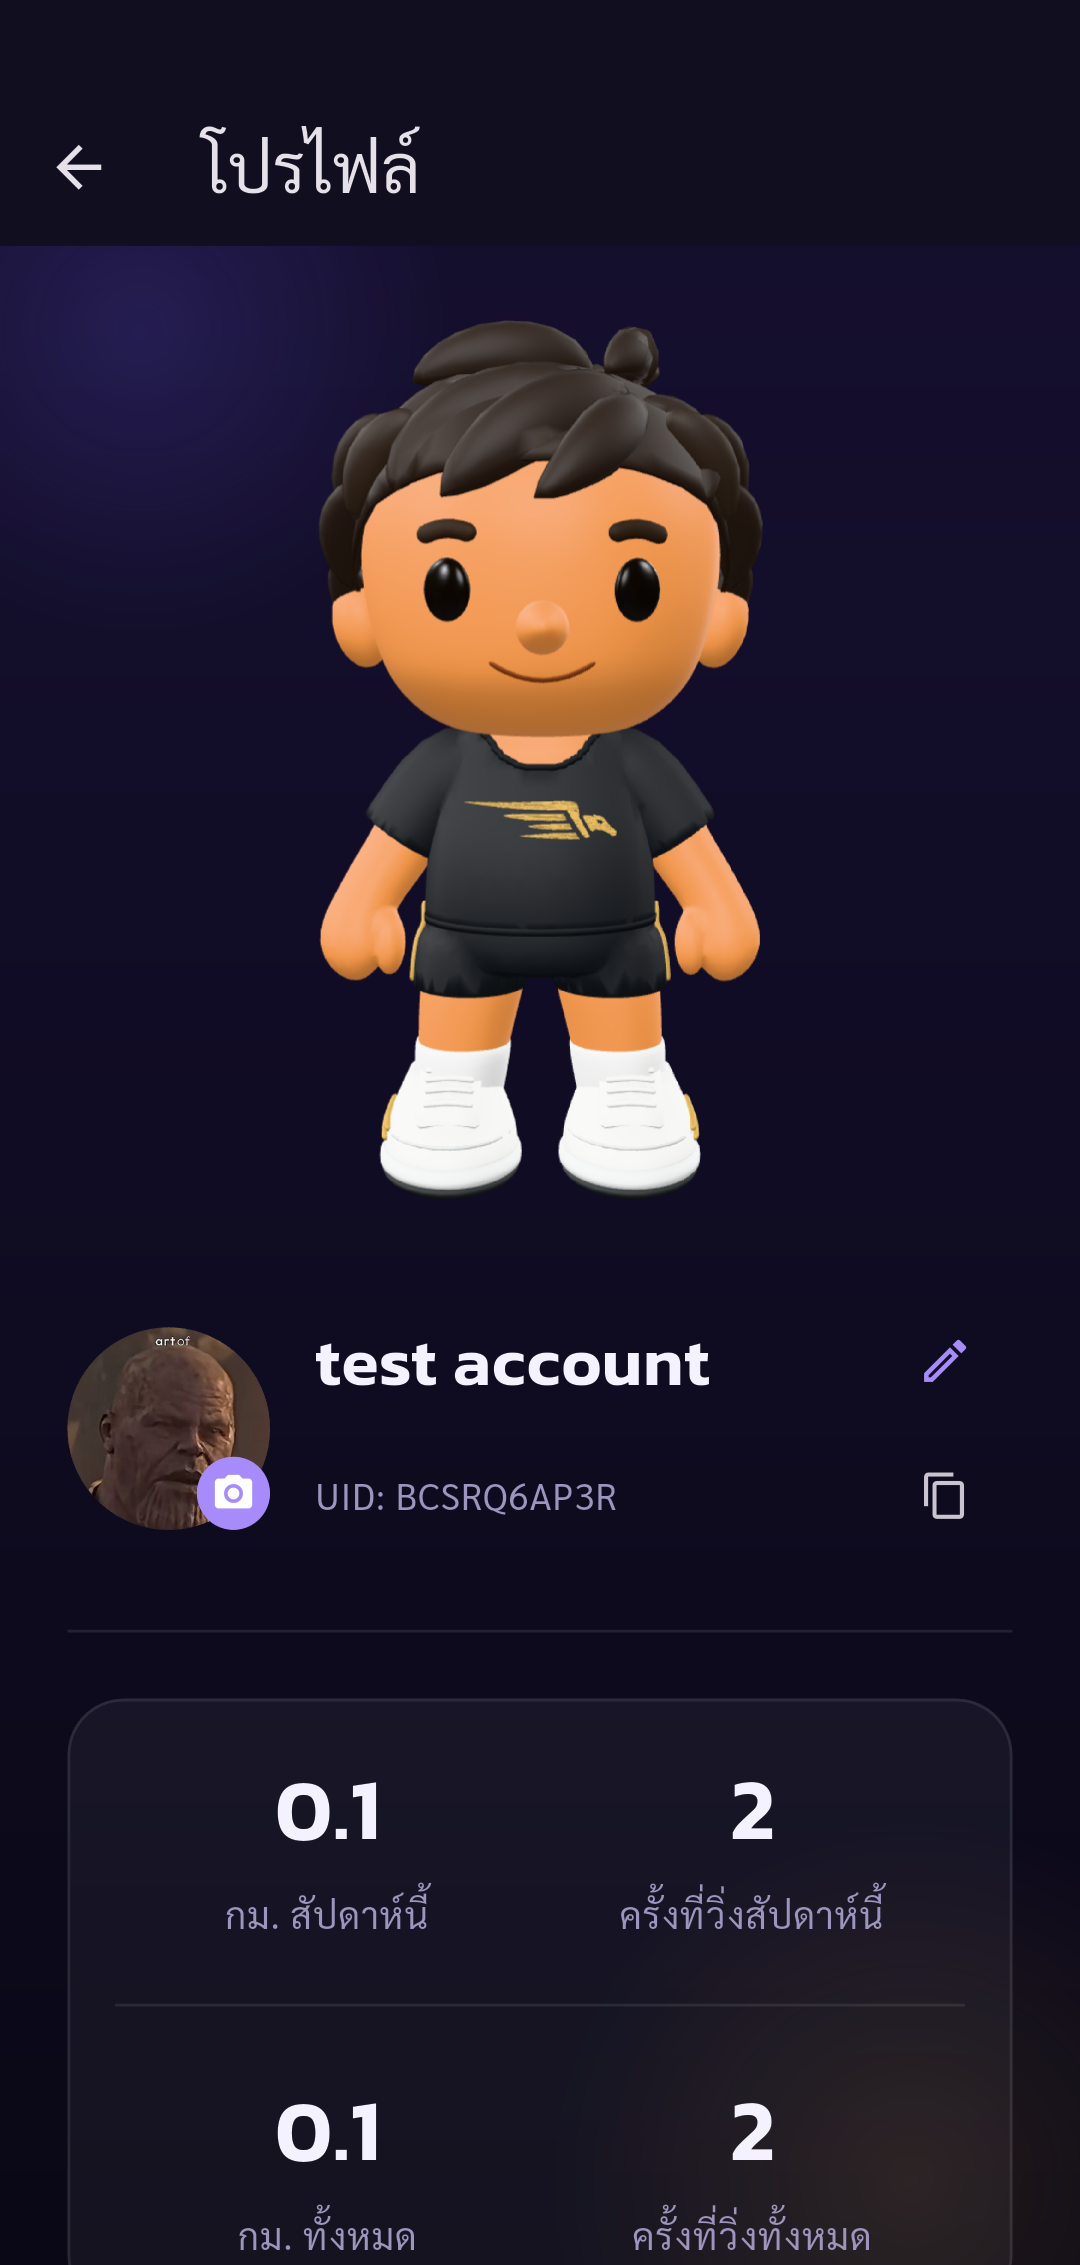
\includegraphics[width=\linewidth,height=0.43\textheight,keepaspectratio]{images/frontend_tests/ft-07-02-photo-persisted.png}
\caption{ภาพใหม่หลังเปิดซ้ำ}\end{subfigure}
\caption{ภาพหลักฐาน FT-07 ชุดที่ 1}\label{fig:flutter-ft-07-1}
\end{figure}

\subsubsection{FT-08 เพื่อน: ส่งคำขอ}

ผลครอบคลุมการปฏิเสธการเพิ่มตนเอง การส่งคำขอด้วย UID ตัวพิมพ์เล็ก การปฏิเสธคำขอซ้ำ และการยกเลิกคำขอ

\begingroup
\small
\renewcommand{\arraystretch}{1.15}
\begin{longtable}{|>{\raggedright\arraybackslash}p{0.07\textwidth}|>{\raggedright\arraybackslash}p{0.57\textwidth}|>{\raggedright\arraybackslash}p{0.08\textwidth}|>{\raggedright\arraybackslash}p{0.16\textwidth}|}
\caption{ผลการทดสอบ FT-08}\label{tab:flutter-ft-08}\\ \hline
\textbf{ลำดับ} & \textbf{จุดตรวจและผลที่ได้รับจริง} & \textbf{ผล} & \textbf{หลักฐาน} \\ \hline
\endfirsthead
\multicolumn{4}{c}{ผลการทดสอบ FT-08 (ต่อ)} \\ \hline
\textbf{ลำดับ} & \textbf{จุดตรวจและผลที่ได้รับจริง} & \textbf{ผล} & \textbf{หลักฐาน} \\ \hline
\endhead
\endfoot
\endlastfoot
1 & แสดงการปฏิเสธจากเซิร์ฟเวอร์เมื่อบัญชีหลักเพิ่ม UID ของตนเอง & ผ่าน & ภาพที่~\ref{fig:flutter-ft-08-1} (a) \\ \hline
2 & รับ UID บัญชีรองที่เป็นตัวพิมพ์เล็ก และแสดงคำขอรอการตอบรับในรายการที่ส่ง & ผ่าน & ภาพที่~\ref{fig:flutter-ft-08-1} (b) \\ \hline
3 & ปฏิเสธการส่งซ้ำ และมีคำขอที่ส่งออกเพียงหนึ่งรายการ & ผ่าน & ภาพที่~\ref{fig:flutter-ft-08-1} (c) \\ \hline
4 & ผู้ส่งยกเลิกแล้วคำขอรอการตอบรับหายจากหน้าจอและข้อมูลความสัมพันธ์จริง & ผ่าน & ภาพที่~\ref{fig:flutter-ft-08-2} (a) \\ \hline
\end{longtable}
\endgroup

\begin{figure}[H]
\centering
\begin{subfigure}[t]{0.31\textwidth}\centering

\includegraphics[width=\linewidth,height=0.43\textheight,keepaspectratio]{images/frontend_tests/ft-08-01-friend-self-rejected.png}
\caption{ปฏิเสธการเพิ่มตนเอง}\end{subfigure}
\hfill
\begin{subfigure}[t]{0.31\textwidth}\centering

\includegraphics[width=\linewidth,height=0.43\textheight,keepaspectratio]{images/frontend_tests/ft-08-02-friend-outgoing.png}
\caption{ส่งคำขอ}\end{subfigure}
\hfill
\begin{subfigure}[t]{0.31\textwidth}\centering

\includegraphics[width=\linewidth,height=0.43\textheight,keepaspectratio]{images/frontend_tests/ft-08-03-friend-duplicate-rejected.png}
\caption{ปฏิเสธคำขอซ้ำ}\end{subfigure}
\caption{ภาพหลักฐาน FT-08 ชุดที่ 1}\label{fig:flutter-ft-08-1}
\end{figure}

\begin{figure}[H]
\centering
\begin{subfigure}[t]{0.31\textwidth}\centering

\includegraphics[width=\linewidth,height=0.43\textheight,keepaspectratio]{images/frontend_tests/ft-08-04-friend-request-cancelled.png}
\caption{ยกเลิกคำขอ}\end{subfigure}
\caption{ภาพหลักฐาน FT-08 ชุดที่ 2}\label{fig:flutter-ft-08-2}
\end{figure}

\subsubsection{FT-09 เพื่อน: บัญชีรองตอบรับ}

รอบนี้ดำเนินการด้วยบัญชีรองเพื่อรับและตอบรับคำขอจากบัญชีหลัก โดยตรวจรหัสความสัมพันธ์ประกอบ

\begingroup
\small
\renewcommand{\arraystretch}{1.15}
\begin{longtable}{|>{\raggedright\arraybackslash}p{0.07\textwidth}|>{\raggedright\arraybackslash}p{0.57\textwidth}|>{\raggedright\arraybackslash}p{0.08\textwidth}|>{\raggedright\arraybackslash}p{0.16\textwidth}|}
\caption{ผลการทดสอบ FT-09}\label{tab:flutter-ft-09}\\ \hline
\textbf{ลำดับ} & \textbf{จุดตรวจและผลที่ได้รับจริง} & \textbf{ผล} & \textbf{หลักฐาน} \\ \hline
\endfirsthead
\multicolumn{4}{c}{ผลการทดสอบ FT-09 (ต่อ)} \\ \hline
\textbf{ลำดับ} & \textbf{จุดตรวจและผลที่ได้รับจริง} & \textbf{ผล} & \textbf{หลักฐาน} \\ \hline
\endhead
\endfoot
\endlastfoot
1 & บัญชีรองเห็นคำขอรอการตอบรับจากบัญชีหลักตรงกับรายการที่ส่งจริง & ผ่าน & ภาพที่~\ref{fig:flutter-ft-09-1} (a) \\ \hline
2 & ผู้รับตอบรับหนึ่งครั้งแล้วเห็นบัญชีหลักในรายการเพื่อน โดยรหัสความสัมพันธ์ตรงกัน & ผ่าน & ภาพที่~\ref{fig:flutter-ft-09-1} (b) \\ \hline
\end{longtable}
\endgroup

\begin{figure}[H]
\centering
\begin{subfigure}[t]{0.31\textwidth}\centering

\includegraphics[width=\linewidth,height=0.43\textheight,keepaspectratio]{images/frontend_tests/ft-09-01-friend-incoming.png}
\caption{คำขอที่ได้รับ}\end{subfigure}
\hfill
\begin{subfigure}[t]{0.31\textwidth}\centering

\includegraphics[width=\linewidth,height=0.43\textheight,keepaspectratio]{images/frontend_tests/ft-09-02-friend-accepted-secondary.png}
\caption{ตอบรับเป็นเพื่อน}\end{subfigure}
\caption{ภาพหลักฐาน FT-09 ชุดที่ 1}\label{fig:flutter-ft-09-1}
\end{figure}

\subsubsection{FT-10 เพื่อน: ตรวจกลับบัญชีหลัก}

กลับมาตรวจบัญชีหลักหลังบัญชีรองตอบรับ โดยไม่สร้างความสัมพันธ์ใหม่ เพื่อยืนยันว่าทั้งสองฝั่งเห็นสถานะตรงกัน

\begingroup
\small
\renewcommand{\arraystretch}{1.15}
\begin{longtable}{|>{\raggedright\arraybackslash}p{0.07\textwidth}|>{\raggedright\arraybackslash}p{0.57\textwidth}|>{\raggedright\arraybackslash}p{0.08\textwidth}|>{\raggedright\arraybackslash}p{0.16\textwidth}|}
\caption{ผลการทดสอบ FT-10}\label{tab:flutter-ft-10}\\ \hline
\textbf{ลำดับ} & \textbf{จุดตรวจและผลที่ได้รับจริง} & \textbf{ผล} & \textbf{หลักฐาน} \\ \hline
\endfirsthead
\multicolumn{4}{c}{ผลการทดสอบ FT-10 (ต่อ)} \\ \hline
\textbf{ลำดับ} & \textbf{จุดตรวจและผลที่ได้รับจริง} & \textbf{ผล} & \textbf{หลักฐาน} \\ \hline
\endhead
\endfoot
\endlastfoot
1 & บัญชีหลักเห็นบัญชีรองเป็นเพื่อนหลังตอบรับ โดยมีความสัมพันธ์เดียวและรหัสตรงกัน & ผ่าน & ภาพที่~\ref{fig:flutter-ft-10-1} (a) \\ \hline
2 & ความสัมพันธ์ที่ตอบรับแล้วไม่ปรากฏเป็นคำขอส่งออกที่รอการตอบรับ & ผ่าน & ภาพที่~\ref{fig:flutter-ft-10-1} (b) \\ \hline
\end{longtable}
\endgroup

\begin{figure}[H]
\centering
\begin{subfigure}[t]{0.31\textwidth}\centering

\includegraphics[width=\linewidth,height=0.43\textheight,keepaspectratio]{images/frontend_tests/ft-10-01-friend-accepted-primary.png}
\caption{เพื่อนในบัญชีหลัก}\end{subfigure}
\hfill
\begin{subfigure}[t]{0.31\textwidth}\centering

\includegraphics[width=\linewidth,height=0.43\textheight,keepaspectratio]{images/frontend_tests/ft-10-02-friend-no-pending-after-accept.png}
\caption{ไม่มีคำขอค้าง}\end{subfigure}
\caption{ภาพหลักฐาน FT-10 ชุดที่ 1}\label{fig:flutter-ft-10-1}
\end{figure}

\subsubsection{FT-11 คลับ: สร้างคลับ}

ผลยืนยันการปฏิเสธชื่อว่างและการสร้างคลับตามข้อมูลทดสอบ โดยบัญชีหลักเป็นหัวหน้าและมีสมาชิกเริ่มต้นหนึ่งคน

\begingroup
\small
\renewcommand{\arraystretch}{1.15}
\begin{longtable}{|>{\raggedright\arraybackslash}p{0.07\textwidth}|>{\raggedright\arraybackslash}p{0.57\textwidth}|>{\raggedright\arraybackslash}p{0.08\textwidth}|>{\raggedright\arraybackslash}p{0.16\textwidth}|}
\caption{ผลการทดสอบ FT-11}\label{tab:flutter-ft-11}\\ \hline
\textbf{ลำดับ} & \textbf{จุดตรวจและผลที่ได้รับจริง} & \textbf{ผล} & \textbf{หลักฐาน} \\ \hline
\endfirsthead
\multicolumn{4}{c}{ผลการทดสอบ FT-11 (ต่อ)} \\ \hline
\textbf{ลำดับ} & \textbf{จุดตรวจและผลที่ได้รับจริง} & \textbf{ผล} & \textbf{หลักฐาน} \\ \hline
\endhead
\endfoot
\endlastfoot
1 & ปฏิเสธชื่อคลับว่าง และไม่สร้างคลับ & ผ่าน & ภาพที่~\ref{fig:flutter-ft-11-1} (a) \\ \hline
2 & บัญชีหลักสร้างคลับตามข้อมูลที่กำหนด เป็นหัวหน้า และมีสมาชิกหนึ่งคน โดยหน้าจอตรงกับ API & ผ่าน & ภาพที่~\ref{fig:flutter-ft-11-1} (b) \\ \hline
\end{longtable}
\endgroup

\begin{figure}[H]
\centering
\begin{subfigure}[t]{0.31\textwidth}\centering
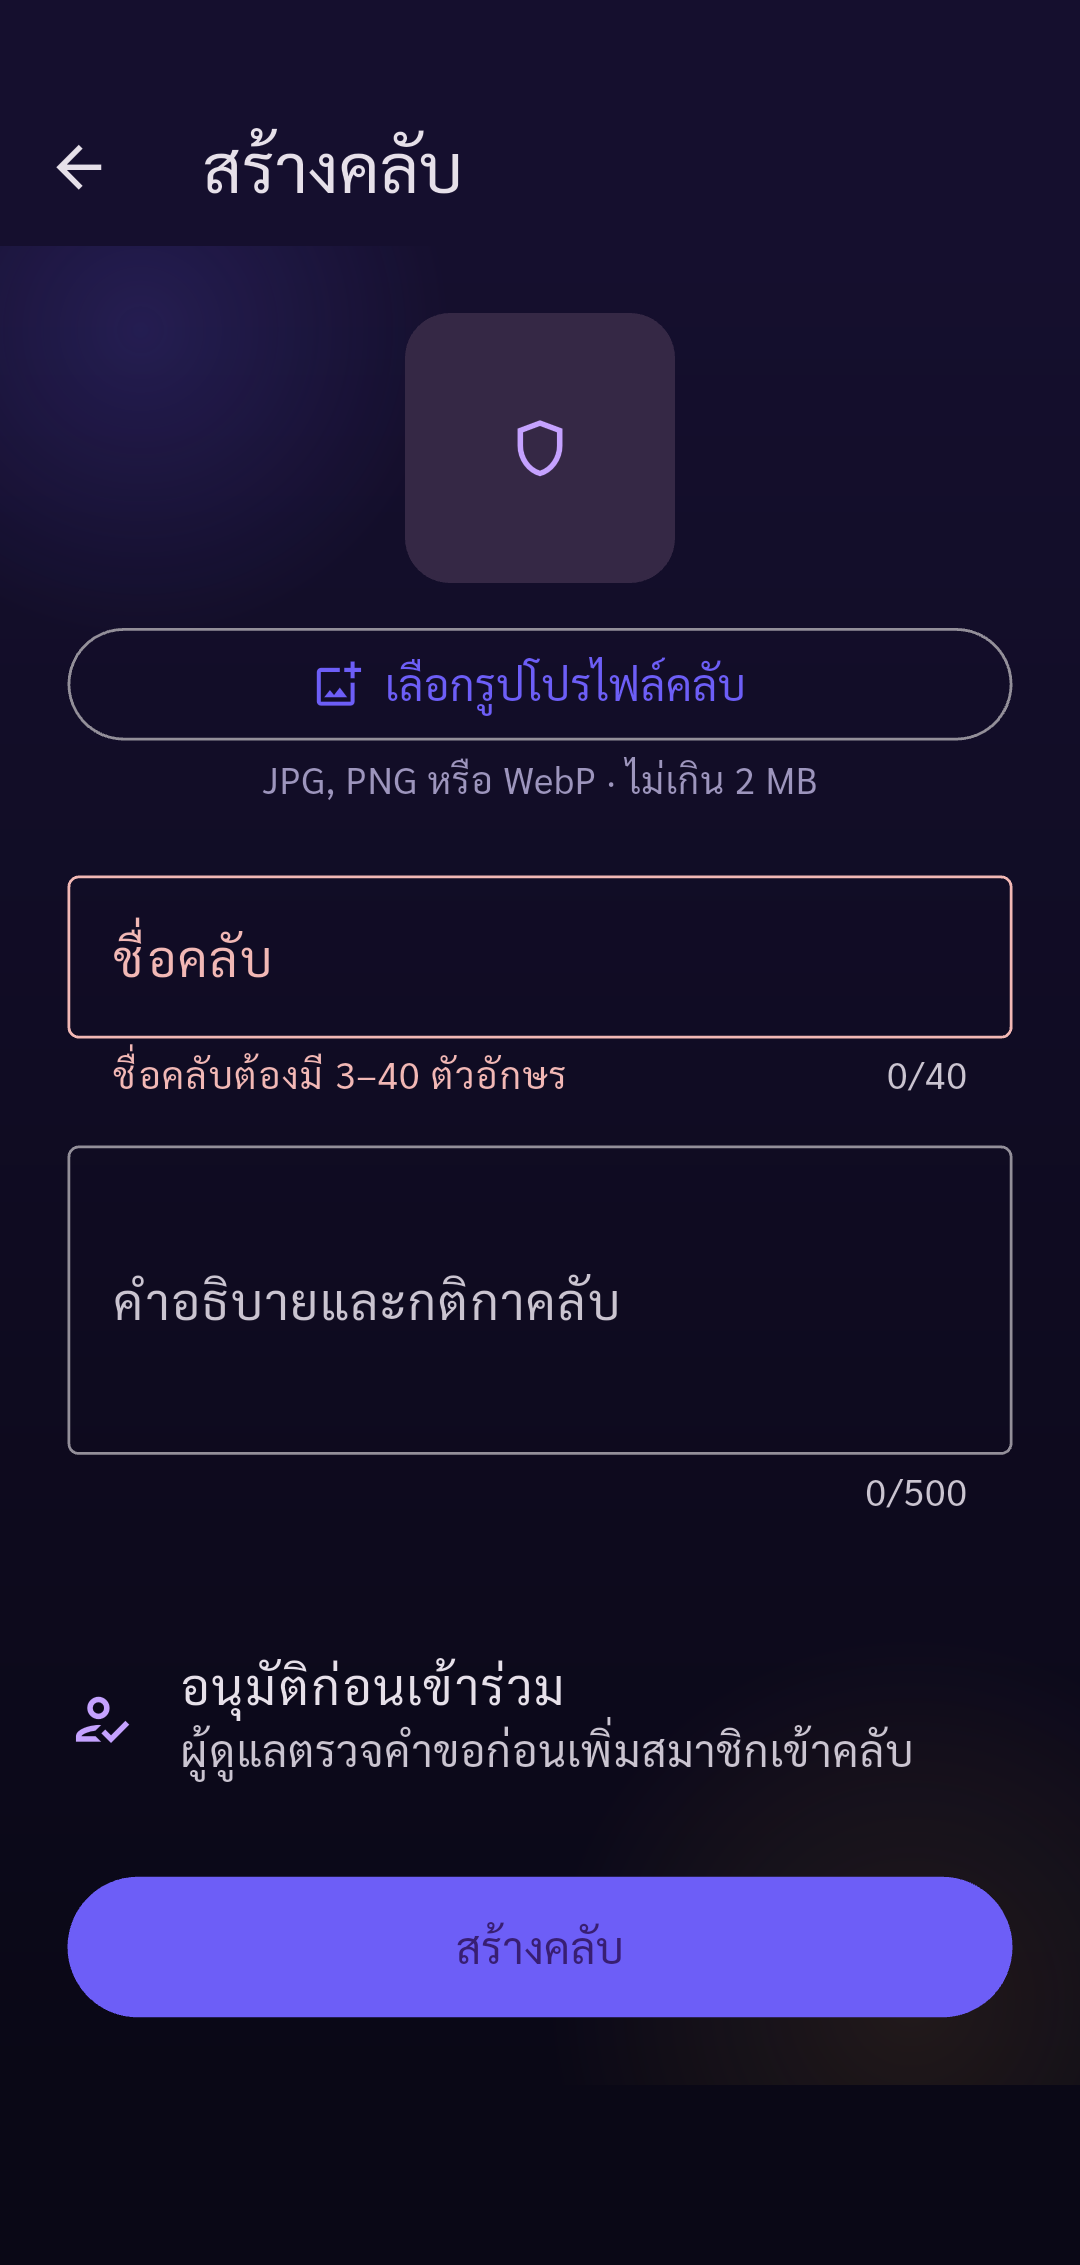
\includegraphics[width=\linewidth,height=0.43\textheight,keepaspectratio]{images/frontend_tests/ft-11-01-club-invalid-name.png}
\caption{ปฏิเสธชื่อคลับว่าง}\end{subfigure}
\hfill
\begin{subfigure}[t]{0.31\textwidth}\centering
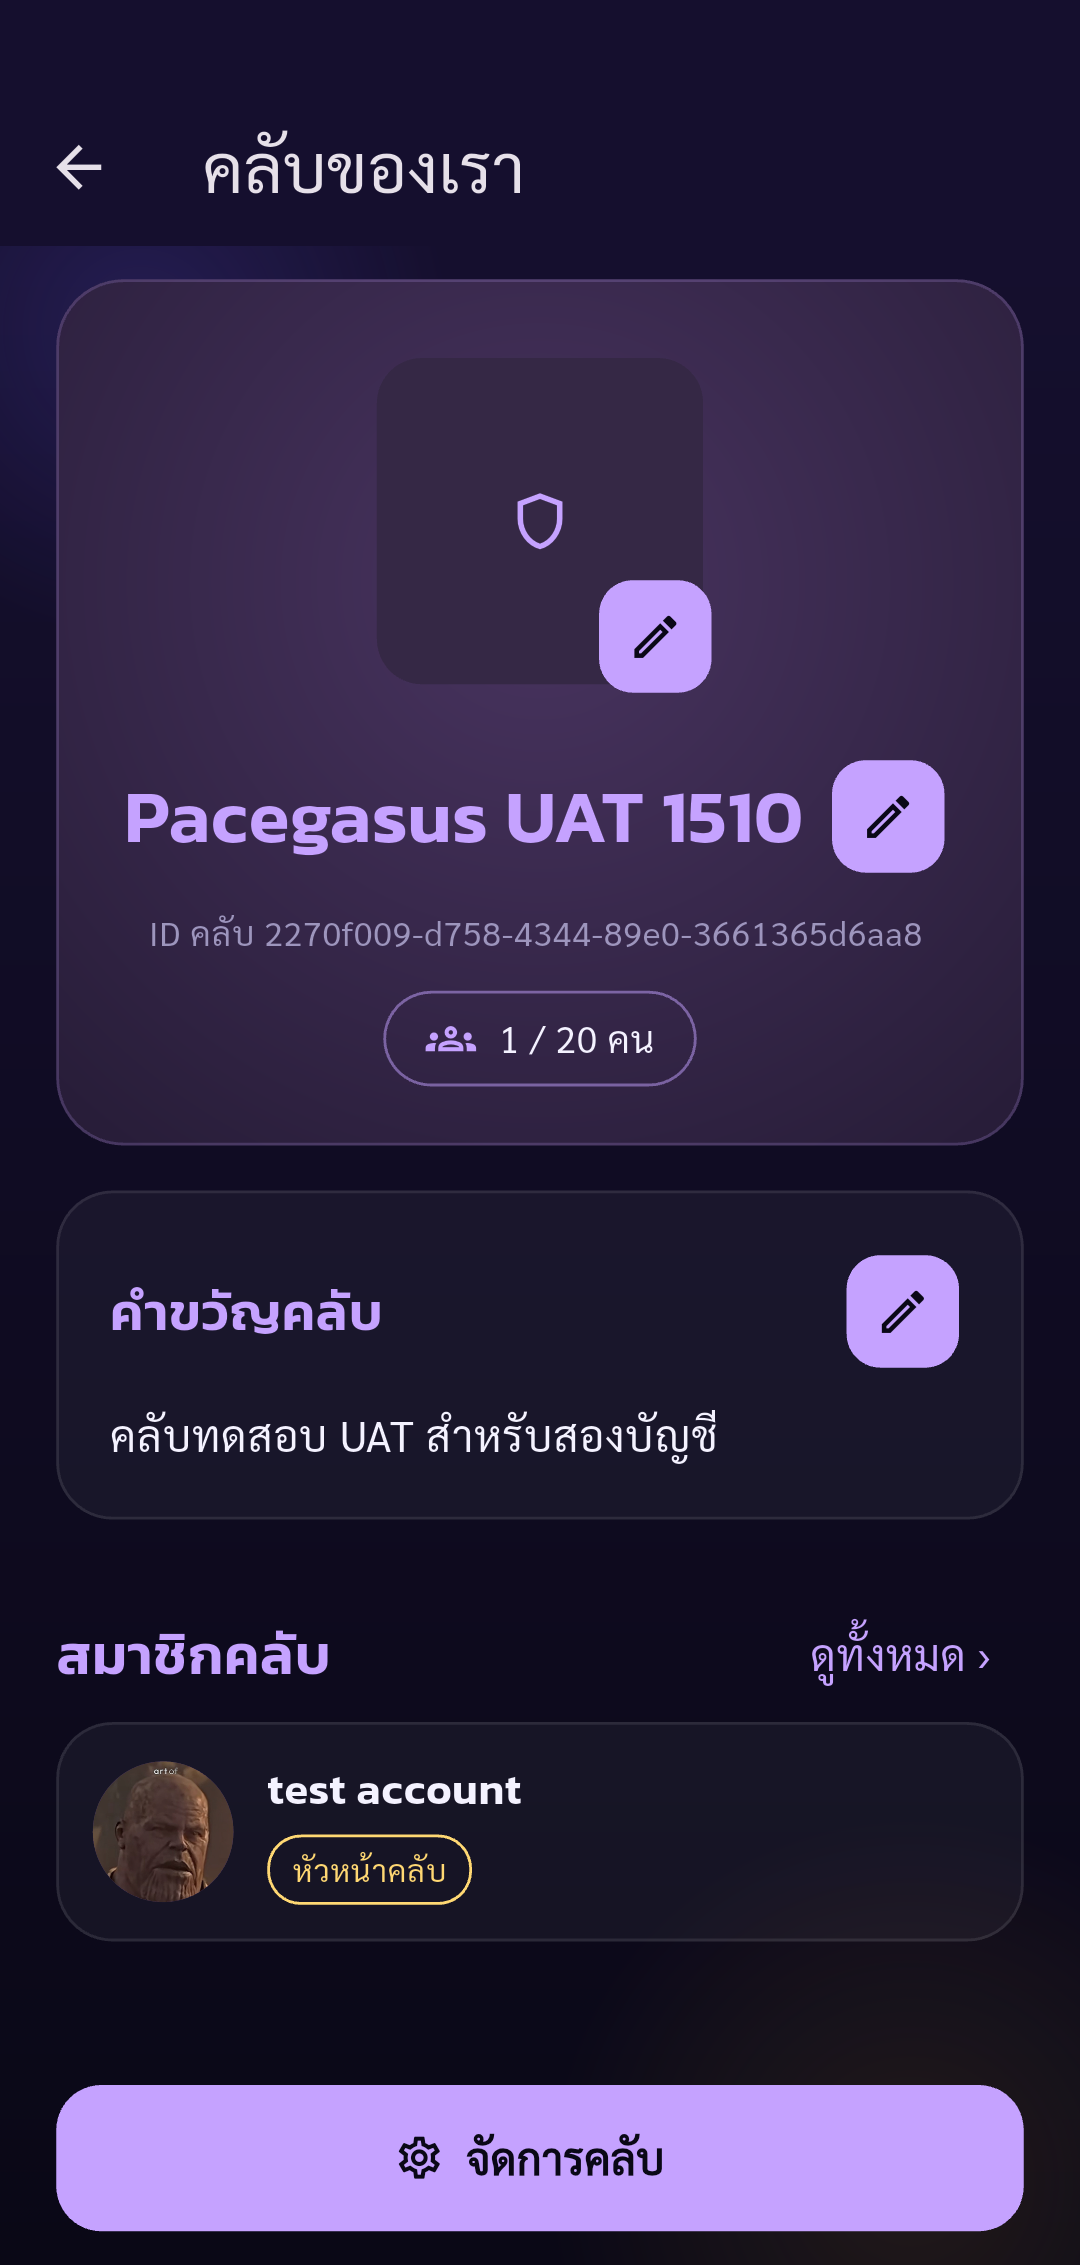
\includegraphics[width=\linewidth,height=0.43\textheight,keepaspectratio]{images/frontend_tests/ft-11-02-club-created.png}
\caption{สร้างคลับสำเร็จ}\end{subfigure}
\caption{ภาพหลักฐาน FT-11 ชุดที่ 1}\label{fig:flutter-ft-11-1}
\end{figure}

\subsubsection{FT-12 คลับ: ค้นหาและขอเข้าร่วม}

ก่อนอนุมัติ บัญชีรองยังไม่เป็นสมาชิกและจำนวนสมาชิกไม่เพิ่ม แม้ส่งคำขอเข้าร่วมสำเร็จแล้ว

\begingroup
\small
\renewcommand{\arraystretch}{1.15}
\begin{longtable}{|>{\raggedright\arraybackslash}p{0.07\textwidth}|>{\raggedright\arraybackslash}p{0.57\textwidth}|>{\raggedright\arraybackslash}p{0.08\textwidth}|>{\raggedright\arraybackslash}p{0.16\textwidth}|}
\caption{ผลการทดสอบ FT-12}\label{tab:flutter-ft-12}\\ \hline
\textbf{ลำดับ} & \textbf{จุดตรวจและผลที่ได้รับจริง} & \textbf{ผล} & \textbf{หลักฐาน} \\ \hline
\endfirsthead
\multicolumn{4}{c}{ผลการทดสอบ FT-12 (ต่อ)} \\ \hline
\textbf{ลำดับ} & \textbf{จุดตรวจและผลที่ได้รับจริง} & \textbf{ผล} & \textbf{หลักฐาน} \\ \hline
\endhead
\endfoot
\endlastfoot
1 & บัญชีรองค้นพบคลับของบัญชีหลักด้วยชื่อผ่านระบบค้นหาจริง & ผ่าน & ภาพที่~\ref{fig:flutter-ft-12-1} (a) \\ \hline
2 & คำขอของบัญชีรองอยู่ระหว่างรออนุมัติ ปุ่มส่งซ้ำถูกปิด ยังไม่เป็นสมาชิก และจำนวนสมาชิกยังเป็นหนึ่งคน & ผ่าน & ภาพที่~\ref{fig:flutter-ft-12-1} (b) \\ \hline
\end{longtable}
\endgroup

\begin{figure}[H]
\centering
\begin{subfigure}[t]{0.31\textwidth}\centering

\includegraphics[width=\linewidth,height=0.43\textheight,keepaspectratio]{images/frontend_tests/ft-12-01-club-search.png}
\caption{ค้นหาคลับ}\end{subfigure}
\hfill
\begin{subfigure}[t]{0.31\textwidth}\centering

\includegraphics[width=\linewidth,height=0.43\textheight,keepaspectratio]{images/frontend_tests/ft-12-02-club-request-pending.png}
\caption{คำขอรออนุมัติ}\end{subfigure}
\caption{ภาพหลักฐาน FT-12 ชุดที่ 1}\label{fig:flutter-ft-12-1}
\end{figure}

\subsubsection{FT-13 คลับ: อนุมัติคำขอ}

ผลหลังอนุมัติยืนยันสมาชิกเพิ่มจากหนึ่งเป็นสองคน มีหัวหน้าหนึ่งคน และคำขอรออนุมัติถูกนำออก

\begingroup
\small
\renewcommand{\arraystretch}{1.15}
\begin{longtable}{|>{\raggedright\arraybackslash}p{0.07\textwidth}|>{\raggedright\arraybackslash}p{0.57\textwidth}|>{\raggedright\arraybackslash}p{0.08\textwidth}|>{\raggedright\arraybackslash}p{0.16\textwidth}|}
\caption{ผลการทดสอบ FT-13}\label{tab:flutter-ft-13}\\ \hline
\textbf{ลำดับ} & \textbf{จุดตรวจและผลที่ได้รับจริง} & \textbf{ผล} & \textbf{หลักฐาน} \\ \hline
\endfirsthead
\multicolumn{4}{c}{ผลการทดสอบ FT-13 (ต่อ)} \\ \hline
\textbf{ลำดับ} & \textbf{จุดตรวจและผลที่ได้รับจริง} & \textbf{ผล} & \textbf{หลักฐาน} \\ \hline
\endhead
\endfoot
\endlastfoot
1 & หัวหน้าคลับเห็นคำขอเข้าร่วมที่รออนุมัติจากบัญชีรอง & ผ่าน & ภาพที่~\ref{fig:flutter-ft-13-1} (a) \\ \hline
2 & อนุมัติแล้วเพิ่มบัญชีรองเป็นสมาชิกเพียงครั้งเดียว มีหัวหน้าหนึ่งคน และคำขอรออนุมัติถูกนำออก & ผ่าน & ภาพที่~\ref{fig:flutter-ft-13-1} (b) \\ \hline
3 & โหลดหน้าคลับของหัวหน้าใหม่แล้วเห็นบัญชีรองเป็นสมาชิก และ API ยืนยันว่ามีสมาชิกทั้งหมดสองคน & ผ่าน & ภาพที่~\ref{fig:flutter-ft-13-1} (c) \\ \hline
\end{longtable}
\endgroup

\begin{figure}[H]
\centering
\begin{subfigure}[t]{0.31\textwidth}\centering

\includegraphics[width=\linewidth,height=0.43\textheight,keepaspectratio]{images/frontend_tests/ft-13-01-club-incoming-request.png}
\caption{คำขอที่หัวหน้าได้รับ}\end{subfigure}
\hfill
\begin{subfigure}[t]{0.31\textwidth}\centering

\includegraphics[width=\linewidth,height=0.43\textheight,keepaspectratio]{images/frontend_tests/ft-13-02-club-approved-request-cleared.png}
\caption{อนุมัติคำขอ}\end{subfigure}
\hfill
\begin{subfigure}[t]{0.31\textwidth}\centering
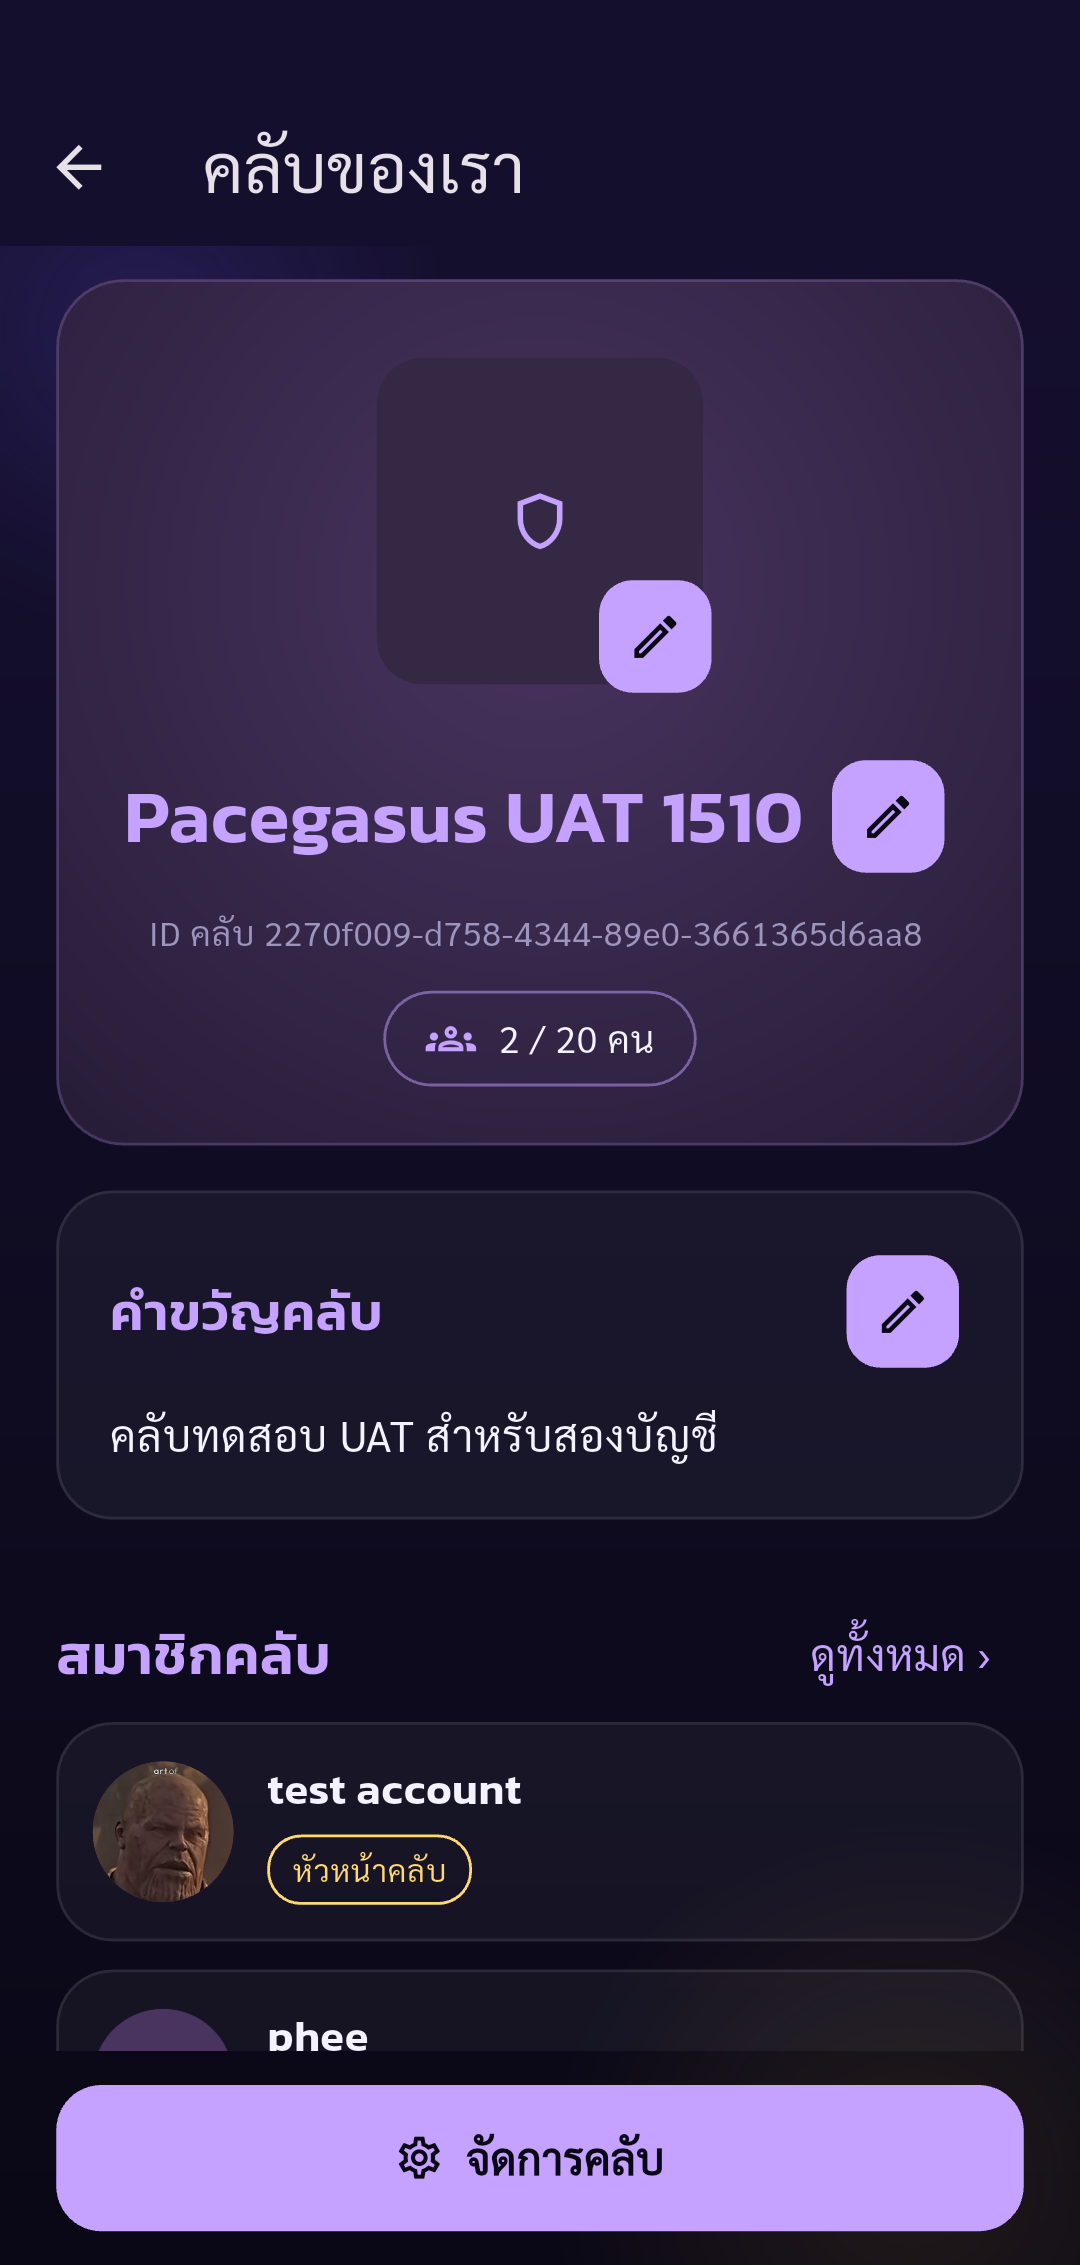
\includegraphics[width=\linewidth,height=0.43\textheight,keepaspectratio]{images/frontend_tests/ft-13-03-club-two-members.png}
\caption{สมาชิกสองคน}\end{subfigure}
\caption{ภาพหลักฐาน FT-13 ชุดที่ 1}\label{fig:flutter-ft-13-1}
\end{figure}

\subsubsection{FT-14 ร้านค้าและ Avatar}

ตามรายงานรวม การซื้อเสื้อสีม่วงราคา 15 เหรียญจากยอด 15 เหรียญทำให้เหลือ 0 เหรียญ และมีรายการซื้อหนึ่งครั้ง ผลการเปิดหน้าหลักและหน้าแต่งตัวซ้ำยืนยันชุดที่บันทึก โดยไม่หักเหรียญเพิ่ม

\begingroup
\small
\renewcommand{\arraystretch}{1.15}
\begin{longtable}{|>{\raggedright\arraybackslash}p{0.07\textwidth}|>{\raggedright\arraybackslash}p{0.57\textwidth}|>{\raggedright\arraybackslash}p{0.08\textwidth}|>{\raggedright\arraybackslash}p{0.16\textwidth}|}
\caption{ผลการทดสอบ FT-14}\label{tab:flutter-ft-14}\\ \hline
\textbf{ลำดับ} & \textbf{จุดตรวจและผลที่ได้รับจริง} & \textbf{ผล} & \textbf{หลักฐาน} \\ \hline
\endfirsthead
\multicolumn{4}{c}{ผลการทดสอบ FT-14 (ต่อ)} \\ \hline
\textbf{ลำดับ} & \textbf{จุดตรวจและผลที่ได้รับจริง} & \textbf{ผล} & \textbf{หลักฐาน} \\ \hline
\endhead
\endfoot
\endlastfoot
1 & ร้านค้าโหลดรายการสินค้าจริงและแสดงยอดเหรียญปัจจุบัน & ผ่าน & ภาพที่~\ref{fig:flutter-ft-14-1} (a) \\ \hline
2 & ปฏิเสธการซื้อเมื่อเหรียญไม่พอ โดยยอดเหรียญ ประวัติซื้อ และความเป็นเจ้าของไม่เปลี่ยน & ผ่าน & ภาพที่~\ref{fig:flutter-ft-14-1} (b) \\ \hline
3 & สินค้าที่เลือกแสดงราคาจริงและภาพตัวอย่าง & ผ่าน & ภาพที่~\ref{fig:flutter-ft-14-1} (c) \\ \hline
4 & ลองสวมสินค้าที่ยังไม่เป็นเจ้าของแล้วเปลี่ยนเฉพาะภาพตัวอย่าง โดยชุดที่บันทึกและความเป็นเจ้าของไม่เปลี่ยน & ผ่าน & ภาพที่~\ref{fig:flutter-ft-14-2} (a) \\ \hline
5 & ซื้อสินค้าที่เลือกแล้วได้รับกรรมสิทธิ์และหักเหรียญตรงราคา (ตรวจบางส่วนของ SFT-07-002) & ผ่าน & ภาพที่~\ref{fig:flutter-ft-14-2} (b) \\ \hline
6 & เลือกสินค้าที่ซื้อแล้วในหน้าแต่งตัว โดยยังไม่บันทึกชุดจริงก่อนกดบันทึก & ผ่าน & ภาพที่~\ref{fig:flutter-ft-14-2} (c) \\ \hline
7 & บันทึกสินค้าที่ซื้อในช่องอุปกรณ์ Avatar ที่ตรงกันได้ (ตรวจบางส่วนของ SFT-07-008) & ผ่าน & ภาพที่~\ref{fig:flutter-ft-14-3} (a) \\ \hline
8 & กลับจากหน้าแต่งตัวแล้วหน้าหลักโหลดชุดที่ซื้อและบันทึกไว้ & ผ่าน & ภาพที่~\ref{fig:flutter-ft-14-3} (b) \\ \hline
9 & เปิดหน้าแต่งตัวใหม่แล้วยังคงชุดที่บันทึก มีรายการซื้อหนึ่งครั้ง และไม่หักเหรียญเพิ่ม & ผ่าน & ภาพที่~\ref{fig:flutter-ft-14-3} (c) \\ \hline
\end{longtable}
\endgroup

\begin{figure}[H]
\centering
\begin{subfigure}[t]{0.31\textwidth}\centering

\includegraphics[width=\linewidth,height=0.43\textheight,keepaspectratio]{images/frontend_tests/ft-14-01-shop-catalog.png}
\caption{รายการสินค้า}\end{subfigure}
\hfill
\begin{subfigure}[t]{0.31\textwidth}\centering
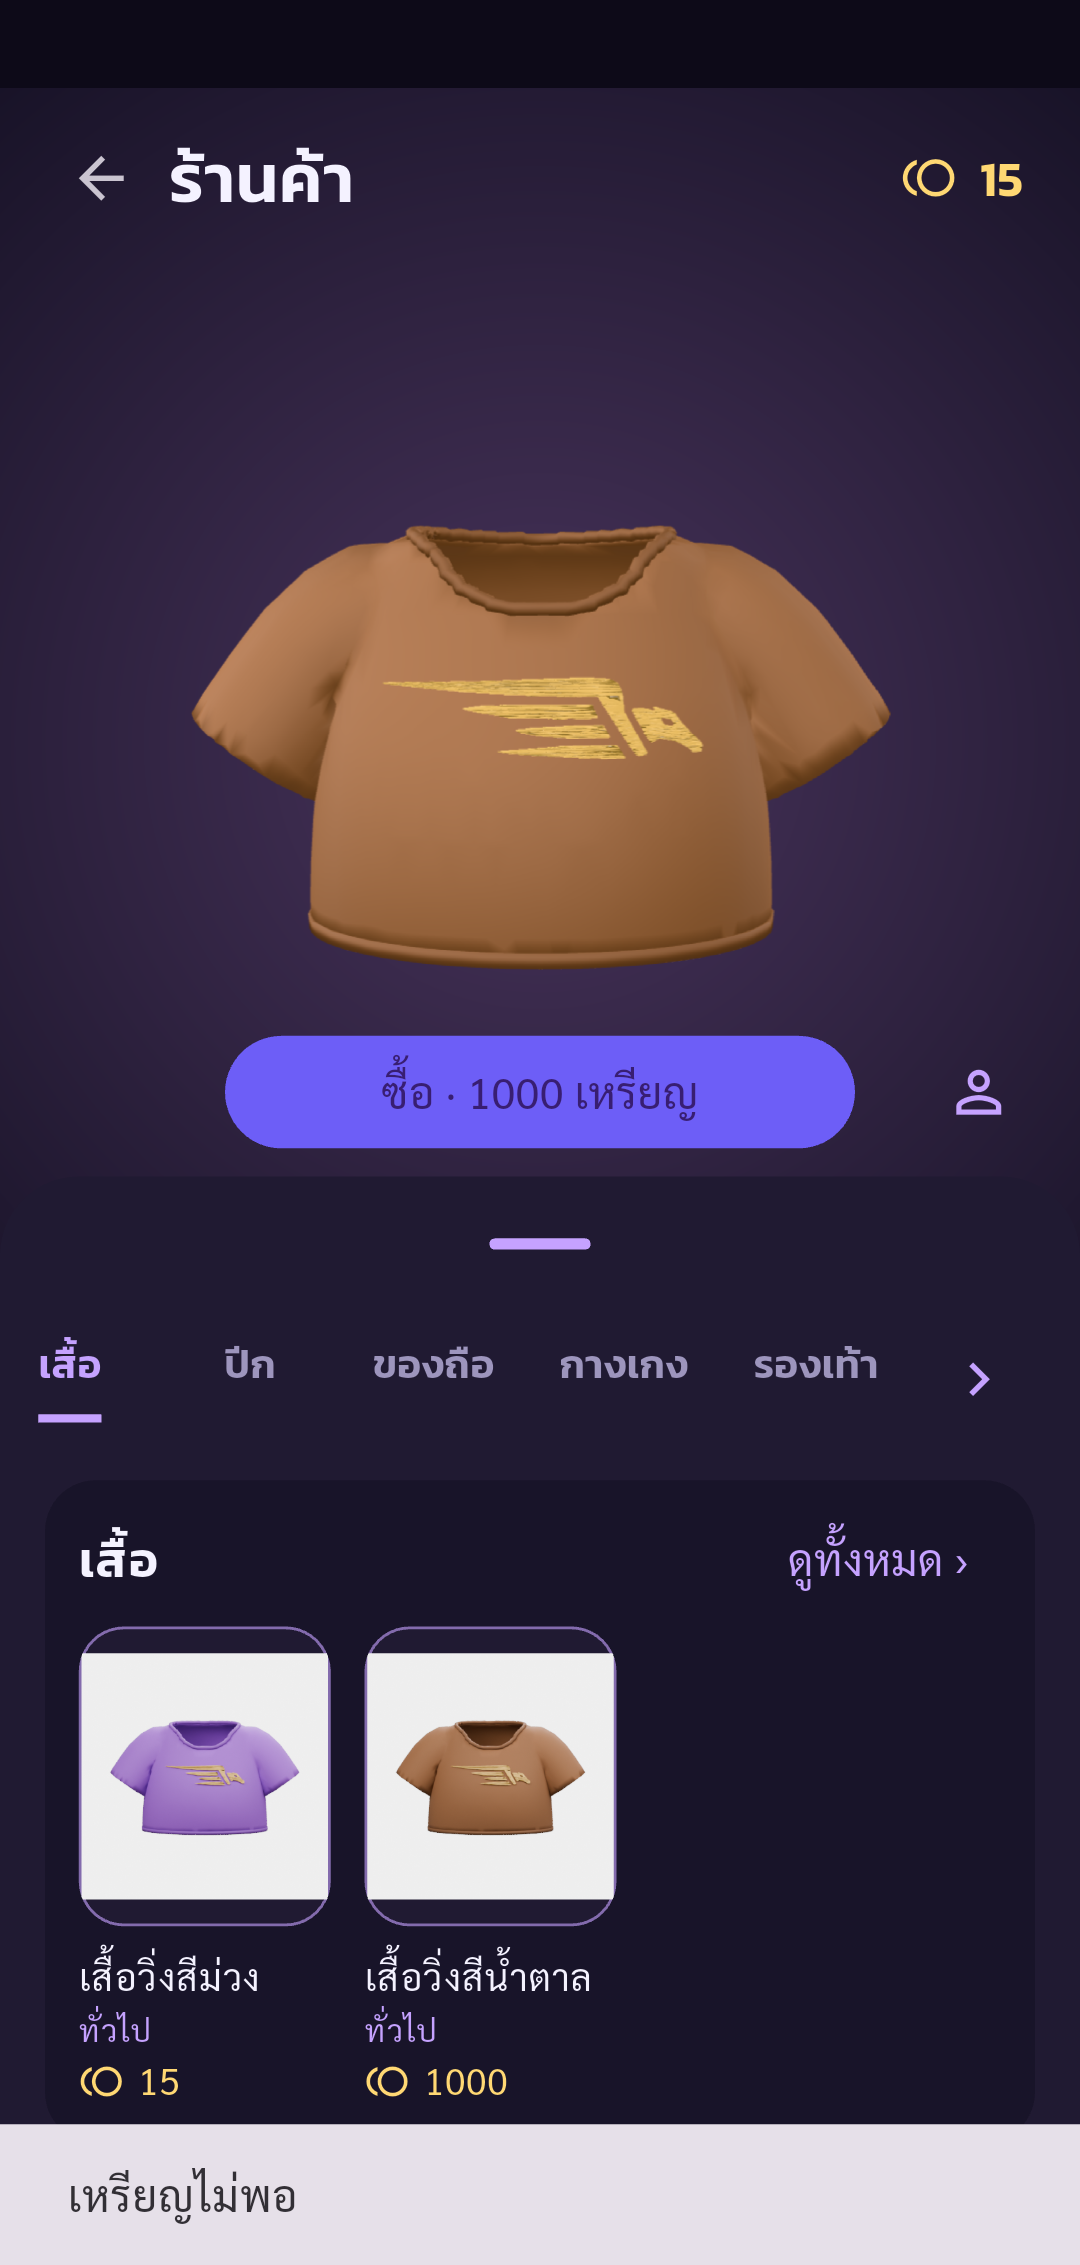
\includegraphics[width=\linewidth,height=0.43\textheight,keepaspectratio]{images/frontend_tests/ft-14-02-shop-insufficient-coins.png}
\caption{เหรียญไม่พอ}\end{subfigure}
\hfill
\begin{subfigure}[t]{0.31\textwidth}\centering
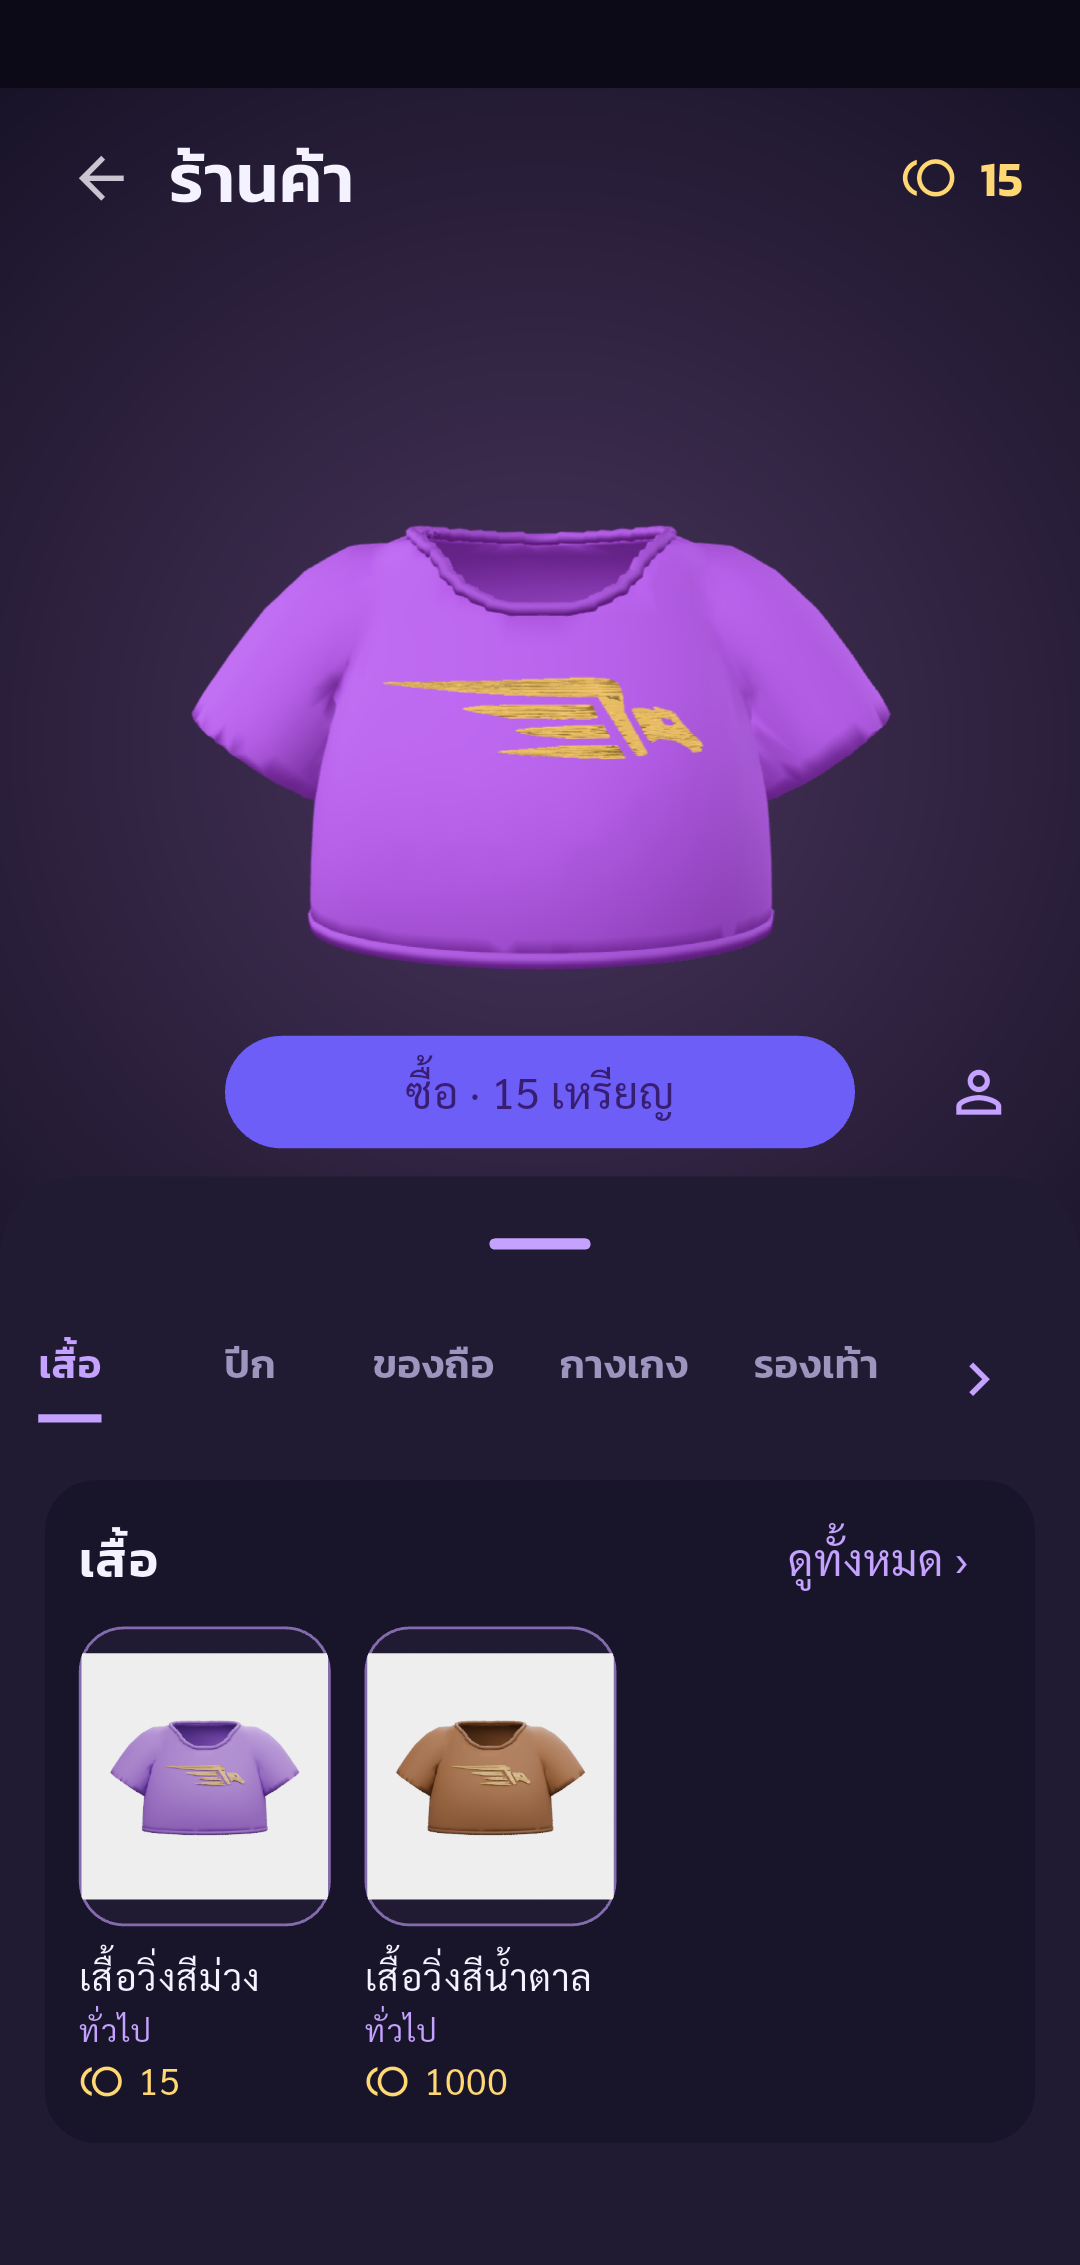
\includegraphics[width=\linewidth,height=0.43\textheight,keepaspectratio]{images/frontend_tests/ft-14-03-shop-product.png}
\caption{ราคาและตัวอย่างสินค้า}\end{subfigure}
\caption{ภาพหลักฐาน FT-14 ชุดที่ 1}\label{fig:flutter-ft-14-1}
\end{figure}

\begin{figure}[H]
\centering
\begin{subfigure}[t]{0.31\textwidth}\centering
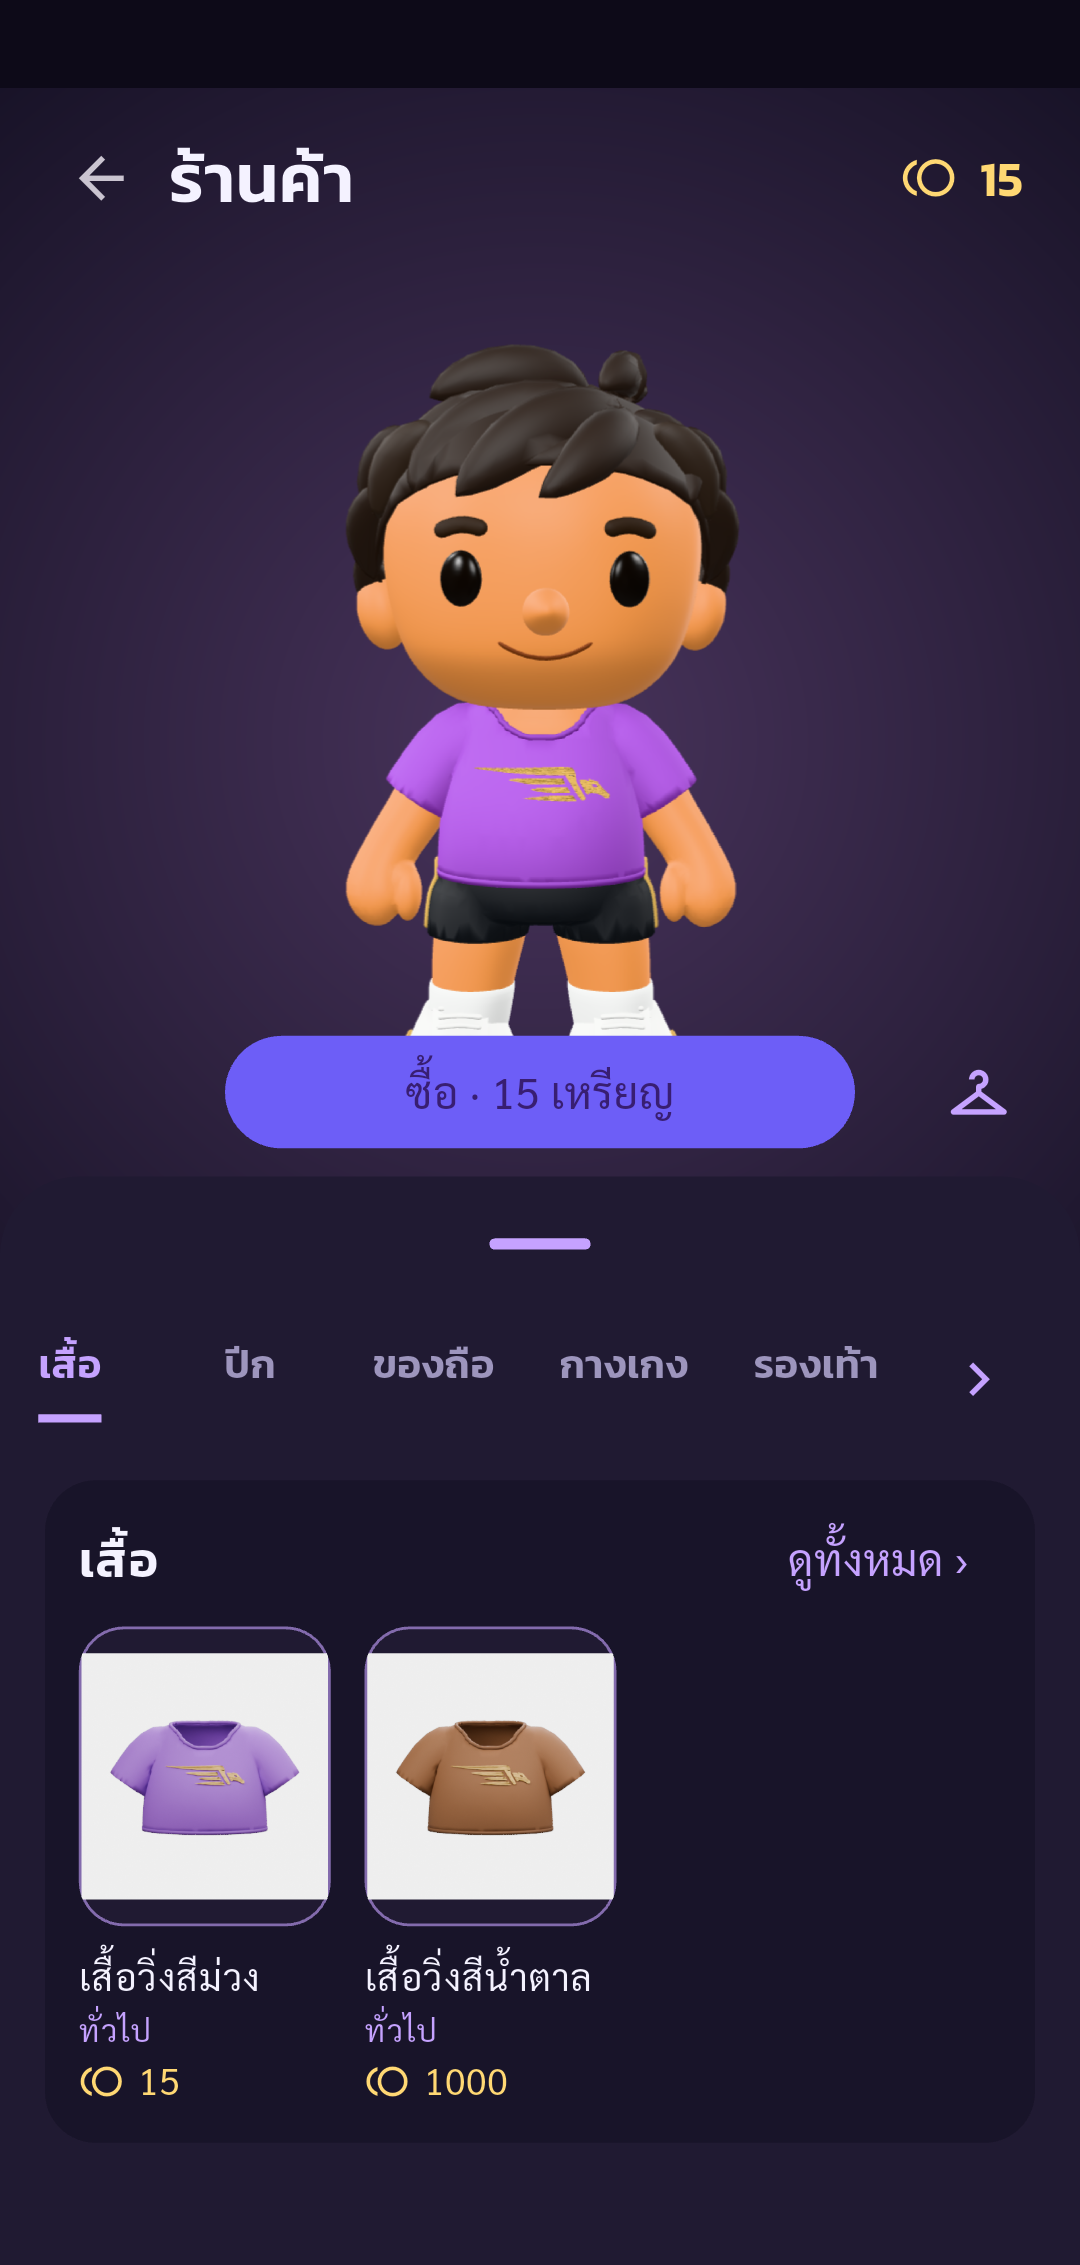
\includegraphics[width=\linewidth,height=0.43\textheight,keepaspectratio]{images/frontend_tests/ft-14-04-shop-try-on.png}
\caption{ลองสวมสินค้า}\end{subfigure}
\hfill
\begin{subfigure}[t]{0.31\textwidth}\centering

\includegraphics[width=\linewidth,height=0.43\textheight,keepaspectratio]{images/frontend_tests/ft-14-05-shop-purchased.png}
\caption{ซื้อสินค้าสำเร็จ}\end{subfigure}
\hfill
\begin{subfigure}[t]{0.31\textwidth}\centering
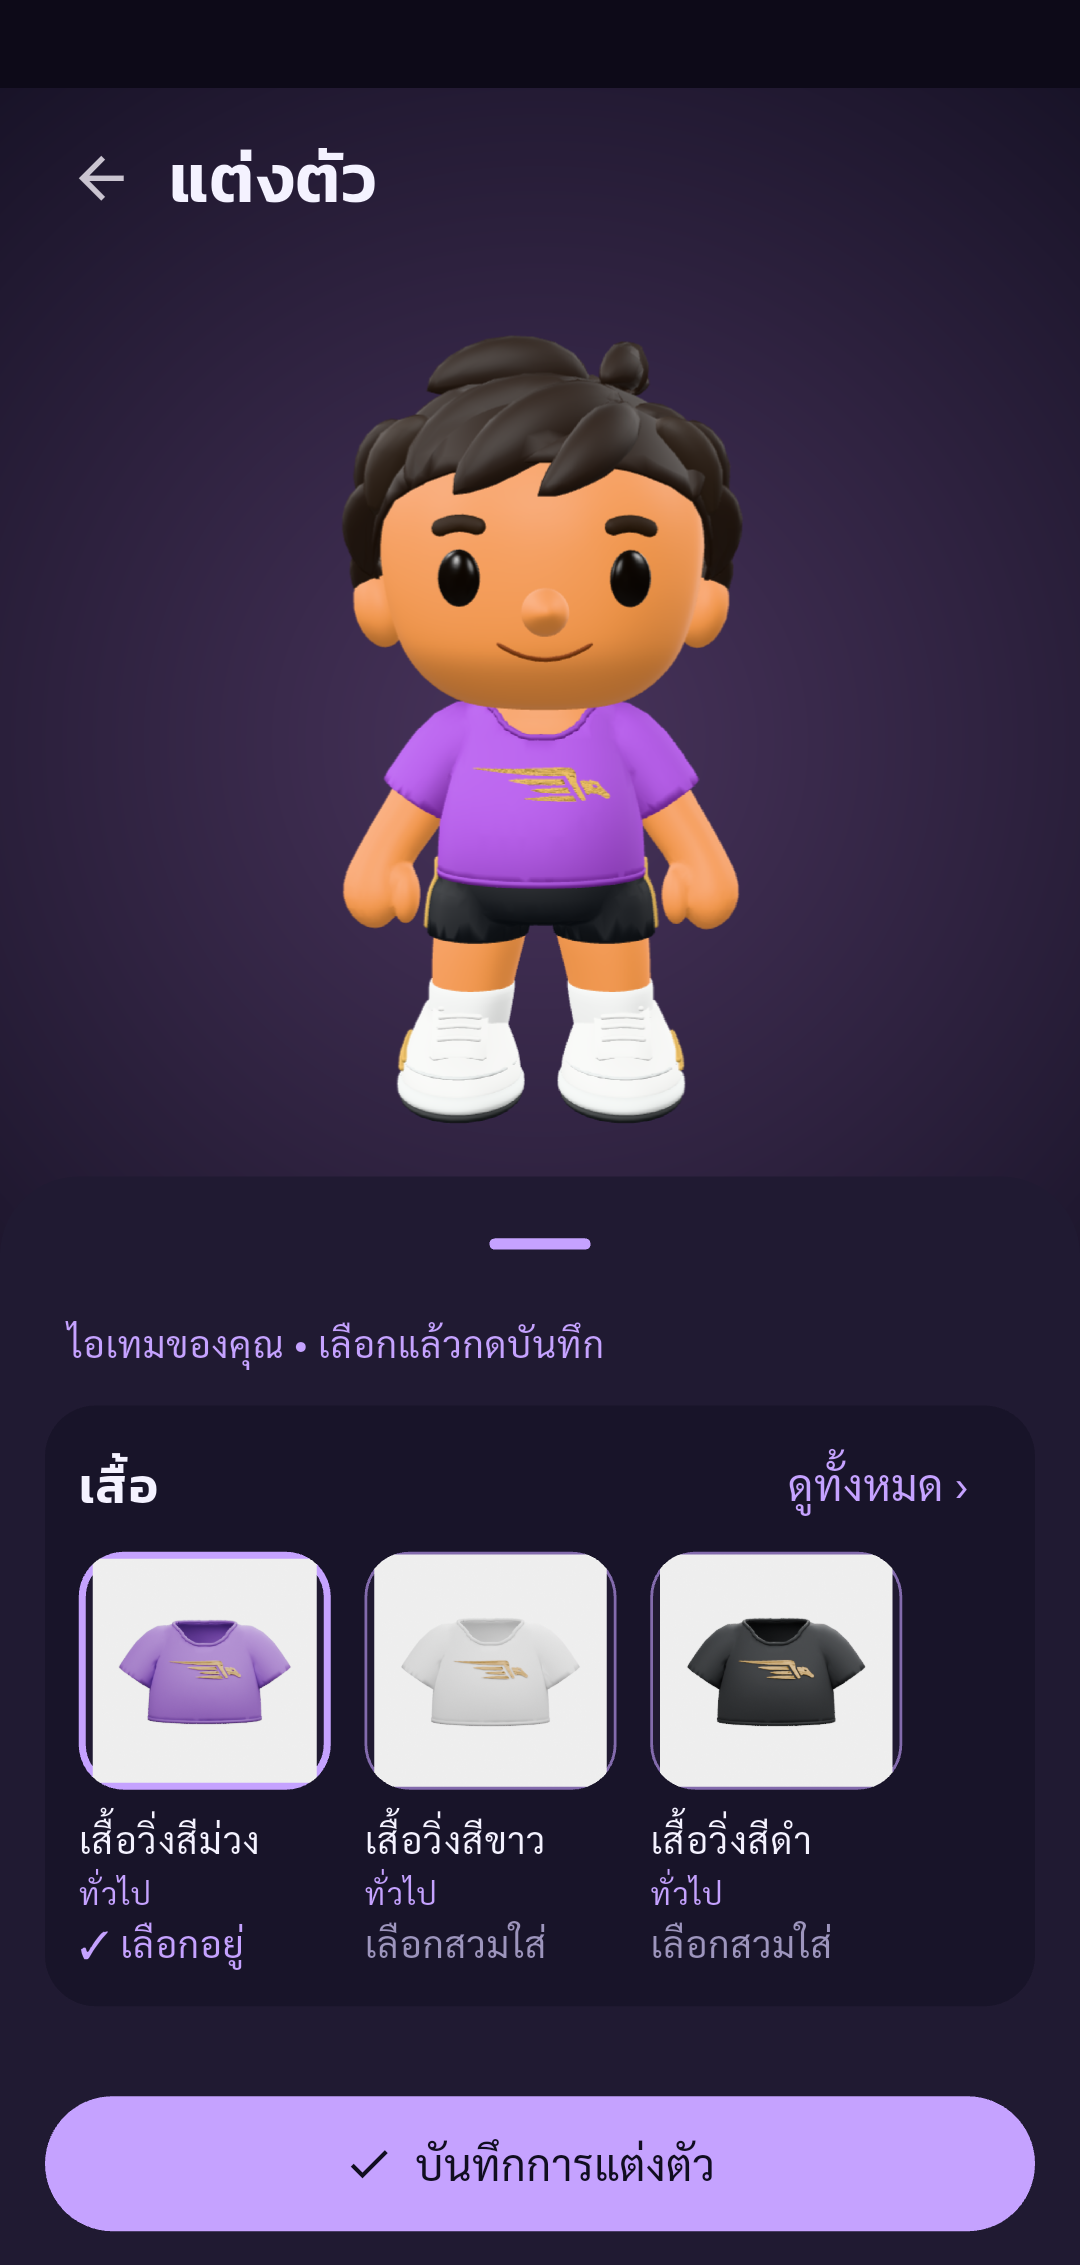
\includegraphics[width=\linewidth,height=0.43\textheight,keepaspectratio]{images/frontend_tests/ft-14-06-avatar-draft.png}
\caption{ชุดที่ยังไม่บันทึก}\end{subfigure}
\caption{ภาพหลักฐาน FT-14 ชุดที่ 2}\label{fig:flutter-ft-14-2}
\end{figure}

\begin{figure}[H]
\centering
\begin{subfigure}[t]{0.31\textwidth}\centering
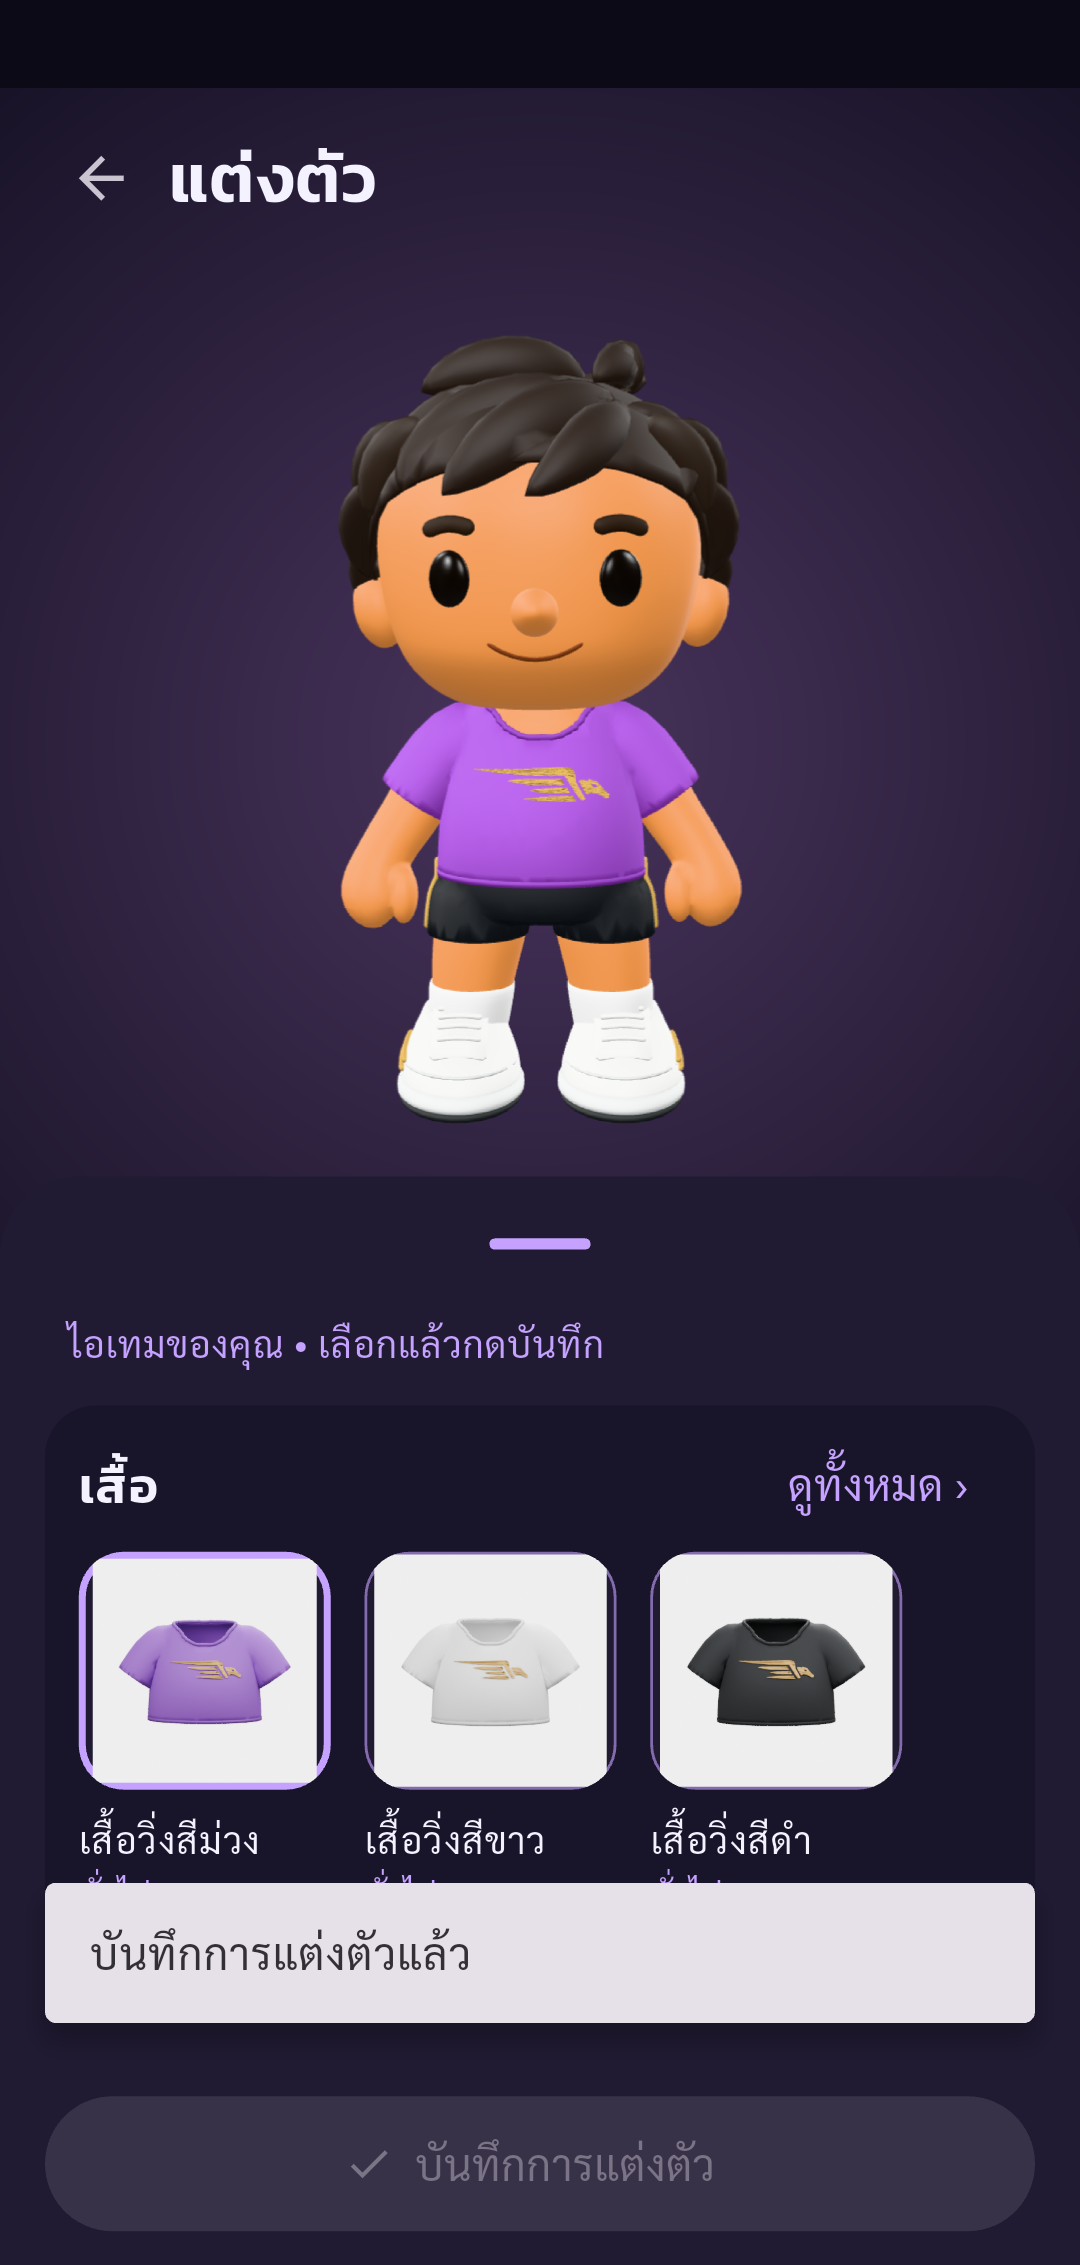
\includegraphics[width=\linewidth,height=0.43\textheight,keepaspectratio]{images/frontend_tests/ft-14-07-shop-equipped.png}
\caption{บันทึกชุด}\end{subfigure}
\hfill
\begin{subfigure}[t]{0.31\textwidth}\centering
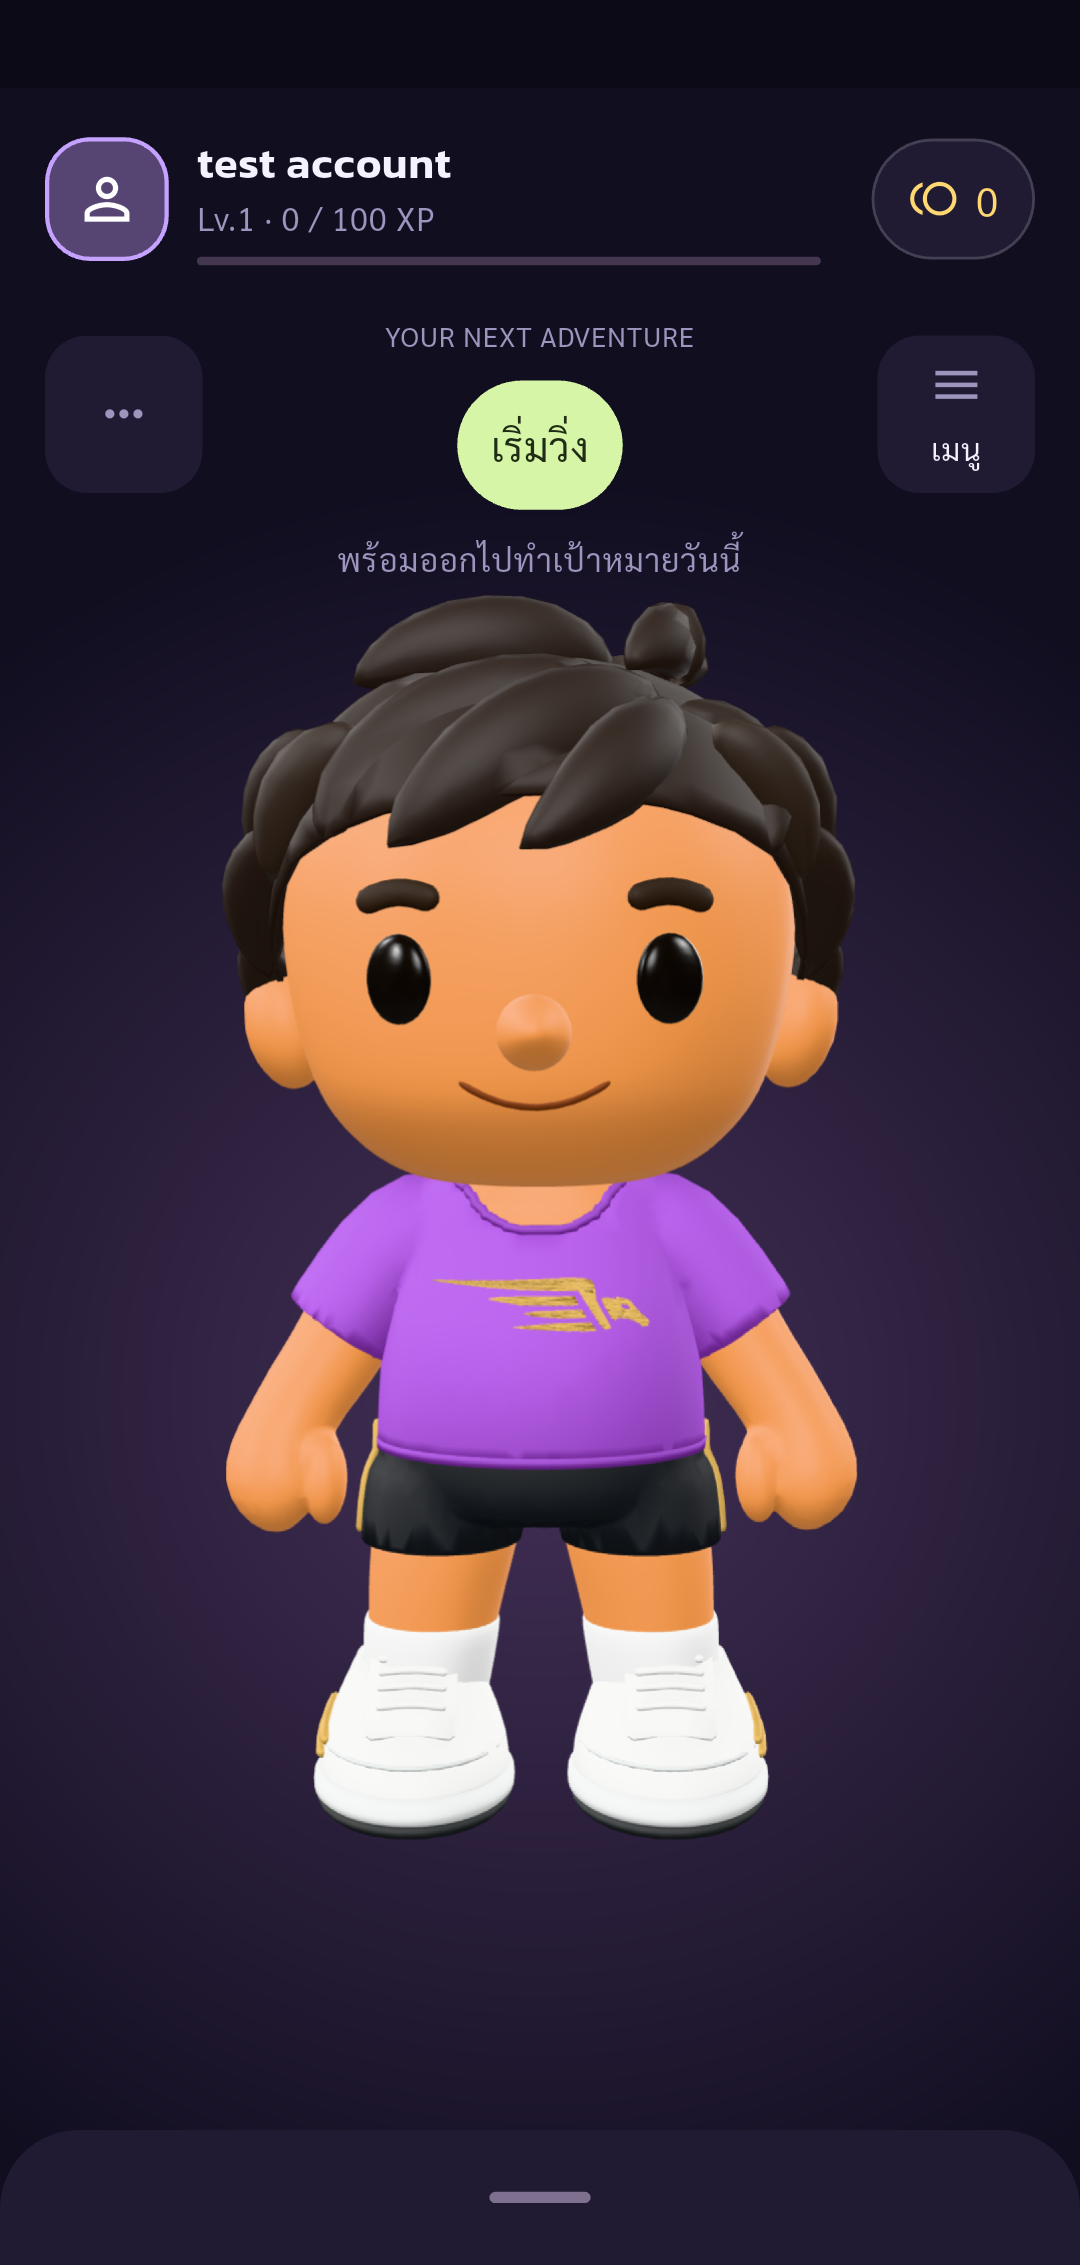
\includegraphics[width=\linewidth,height=0.43\textheight,keepaspectratio]{images/frontend_tests/ft-14-08-avatar-home.png}
\caption{ชุดบนหน้าหลัก}\end{subfigure}
\hfill
\begin{subfigure}[t]{0.31\textwidth}\centering
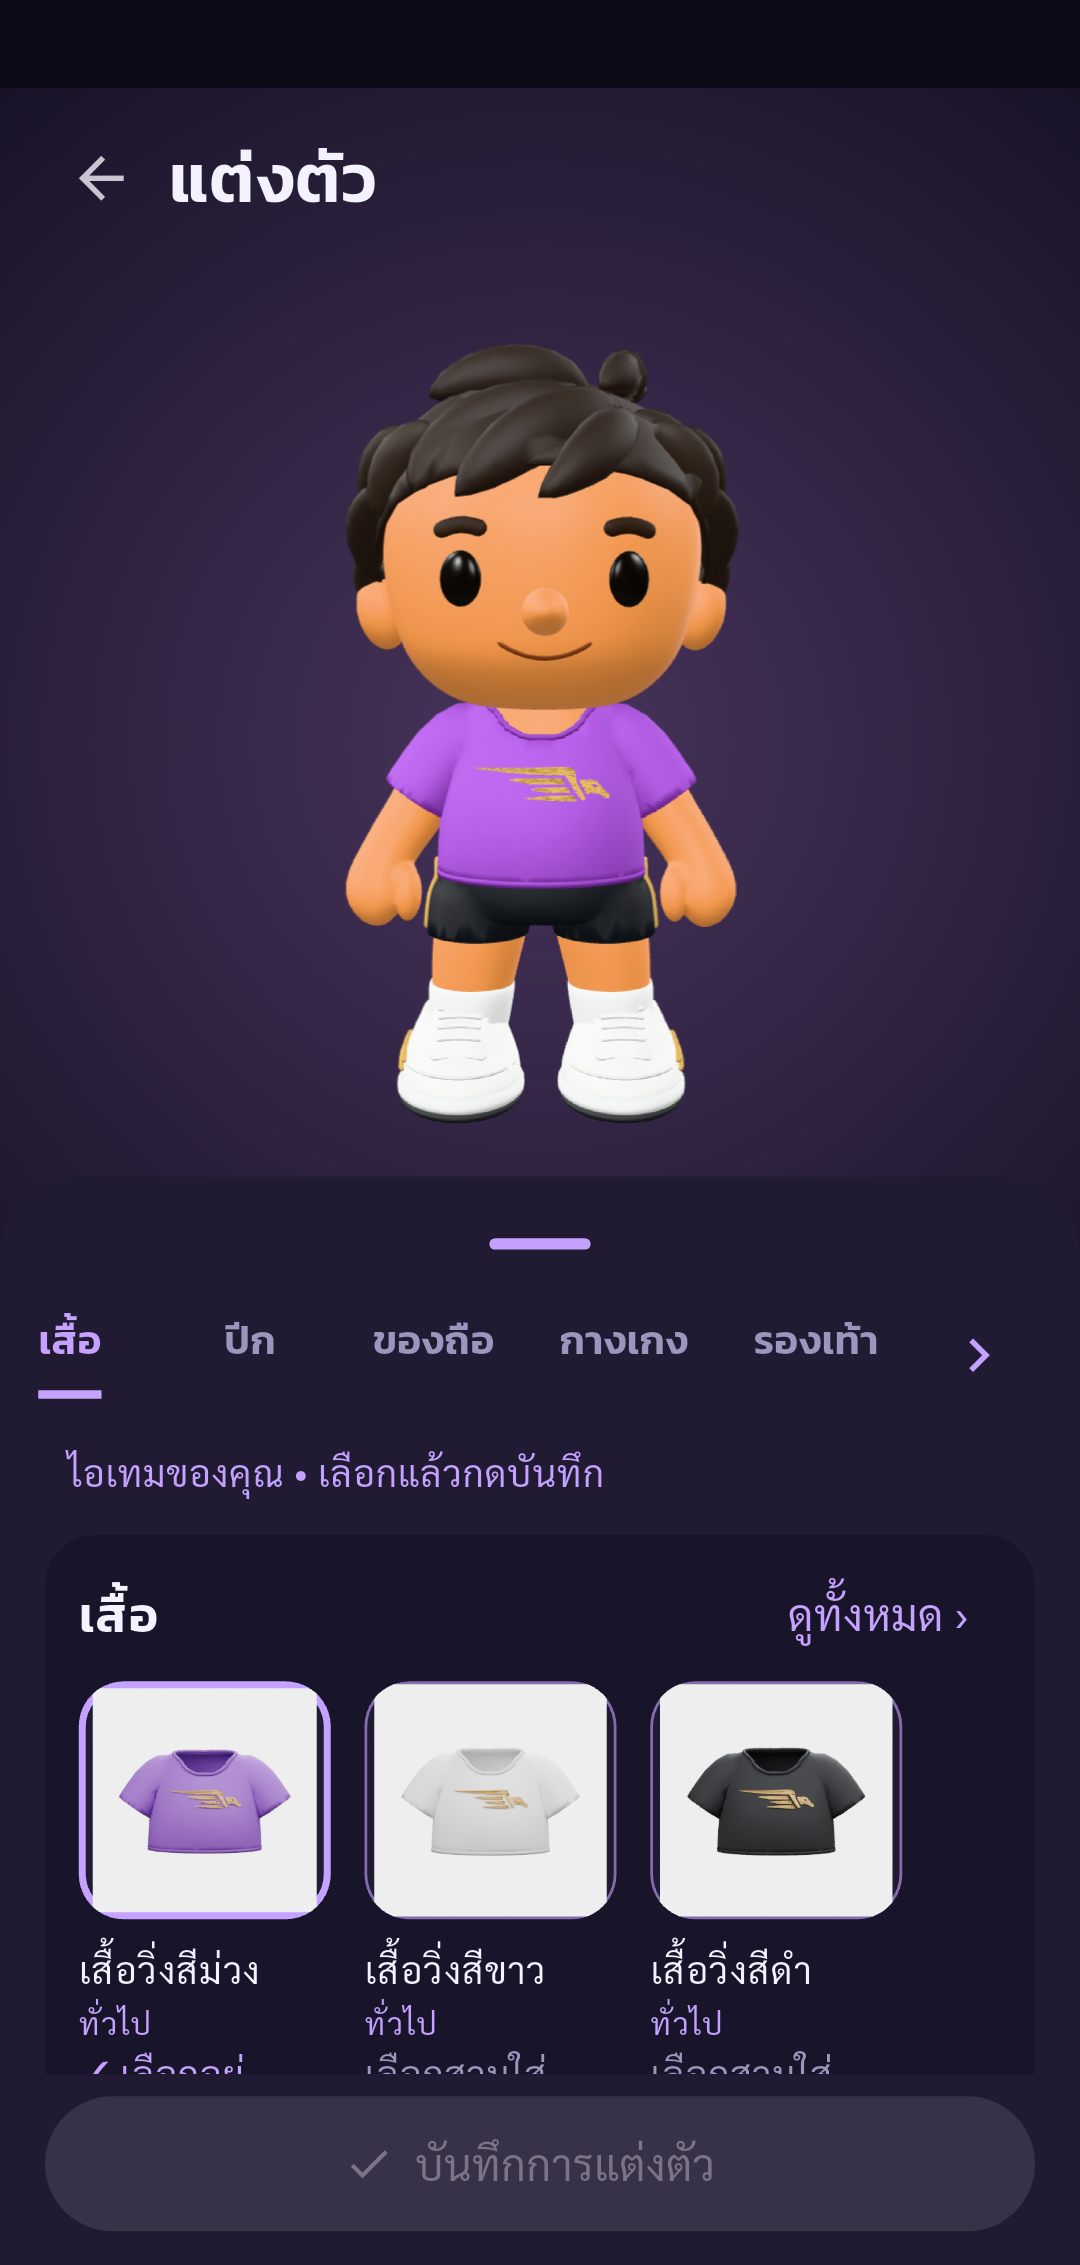
\includegraphics[width=\linewidth,height=0.43\textheight,keepaspectratio]{images/frontend_tests/ft-14-09-avatar-reopened.png}
\caption{เปิดหน้าแต่งตัวซ้ำ}\end{subfigure}
\caption{ภาพหลักฐาน FT-14 ชุดที่ 3}\label{fig:flutter-ft-14-3}
\end{figure}

